\documentclass{article}
\usepackage{graphicx}
\usepackage{titlesec}
\usepackage{hyperref}
\usepackage{caption}
\usepackage{listings}
\usepackage{xcolor}
\usepackage[a4paper, margin=1in]{geometry}
\usepackage{float}
\usepackage{tocloft}

\cftsetindents{subsection}{1.5em}{2.3em}
\setlength{\cftsecnumwidth}{4em}
\setlength{\cftsubsecnumwidth}{5em}

\titleformat{\section}
  {\Large\bfseries}
  {Exercise \arabic{section}.}
  {1em}
  {}

\raggedbottom
\setlength{\intextsep}{6pt plus 2pt minus 2pt}
\setlength{\floatsep}{6pt plus 2pt minus 2pt}
\setlength{\textfloatsep}{6pt plus 2pt minus 2pt}

\begin{document}

\begin{titlepage}
    \centering
    
\includegraphics[width=0.4\textwidth]{./screenshots/Epita.jpg} \\
    \vspace{1.5cm}

    {\large Master in Computer Science} \\
    {\large Big Data Infrastructure and Cloud Computing} \\

    \vspace{0.5cm}
    {\Huge \textbf{Hadoop MapReduce Implementation}} \\
    \vspace{1.3cm}
    {\huge Lab 8 Report} \\
    \vspace{0.1cm}
    {\Large Exercises 1--12} \\

    \vspace{1.5cm}
    {\Large \textbf{Student}} \\
    \vspace{0.5cm}
    {\large Arihant Jain} \\

    \vspace{1.5cm}
    {\large April 2026}
\end{titlepage}

\tableofcontents
\newpage

\section*{Project Setup}
\addcontentsline{toc}{section}{Project Setup}

The provided project was imported into the \texttt{lab\_8} folder, built with Maven, and run locally with Hadoop. The sample commands and outputs were captured for the report.

\begin{figure}[H]
    \centering
    
\includegraphics[width=0.75\textwidth]{screenshots/phase3/compile.png}
    \caption{Maven build for the project}
\end{figure}

\section{Word Count (Single File)}

\subsection*{Objective}
Count the occurrences of each word in one input file.

\subsection*{Implementation}
The mapper splits each line into words and emits each word with value \texttt{1}. The reducer sums the values for each word.

\subsection*{Result}
The output lists the total count for each word in the file.

\begin{figure}[H]
    \centering
    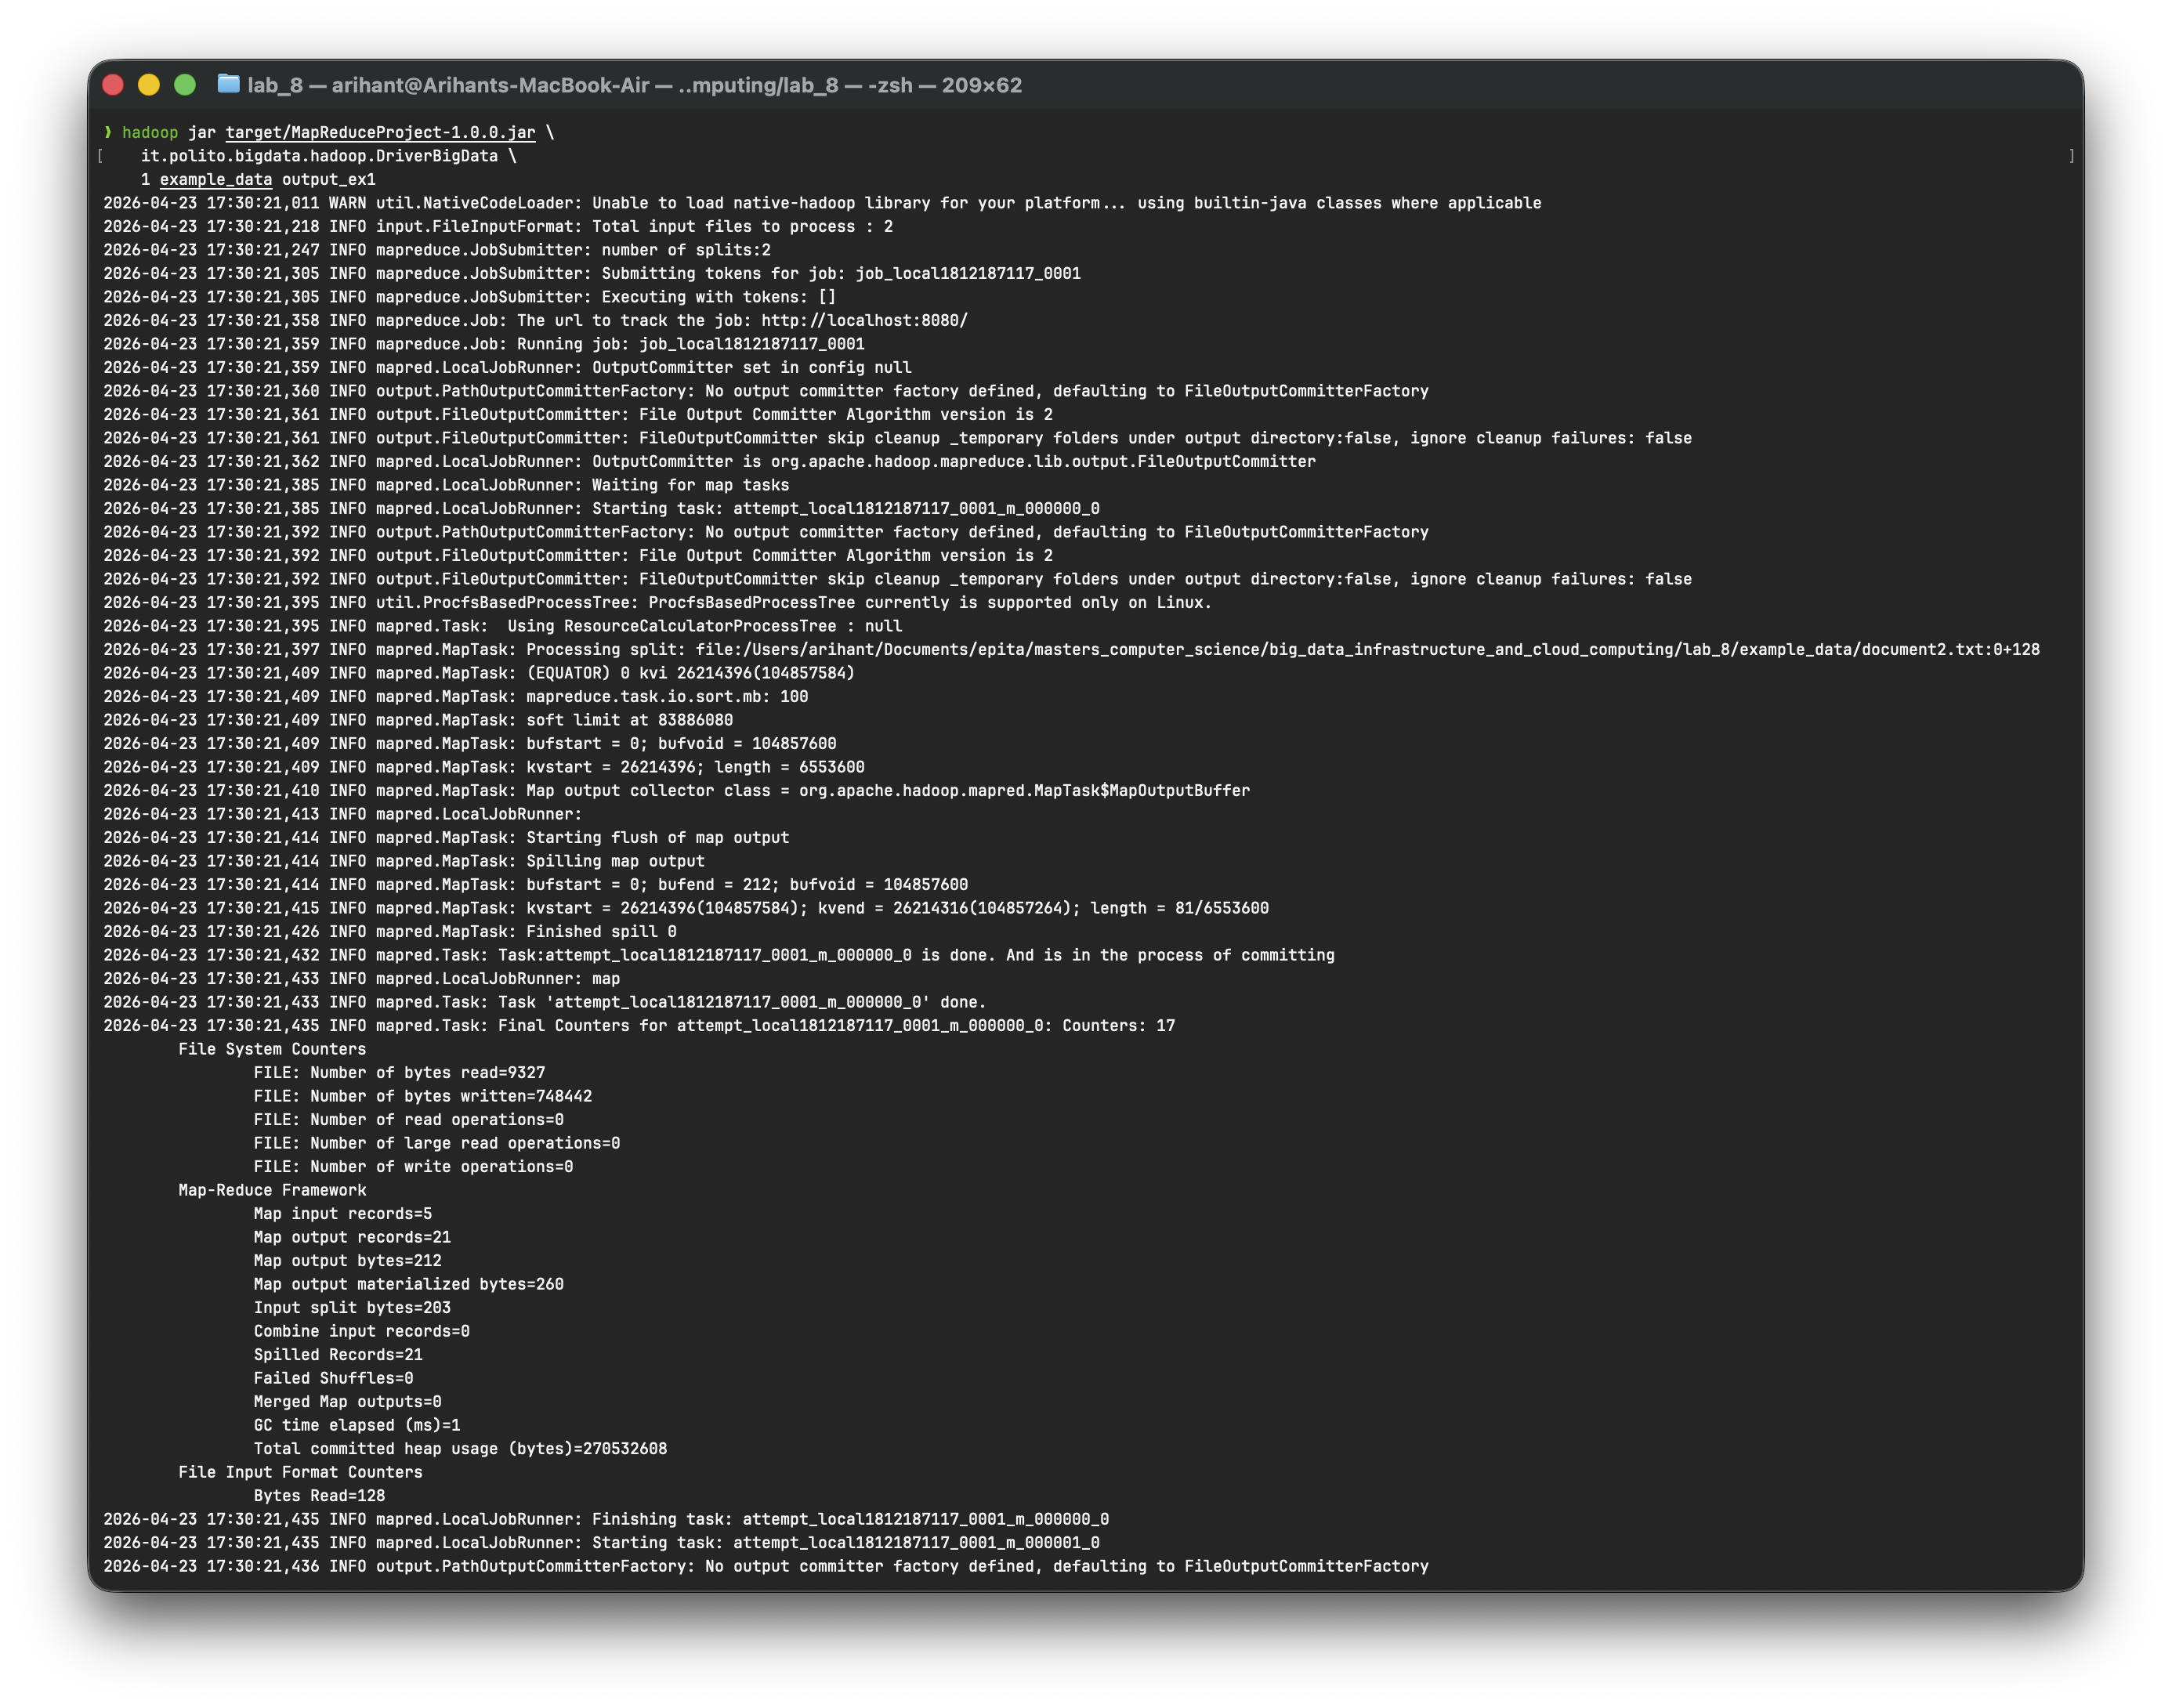
\includegraphics[width=0.75\textwidth]{screenshots/phase1/hadoop_cmd.png}
    \caption{Exercise 1 command}
\end{figure}

\begin{figure}[H]
    \centering
    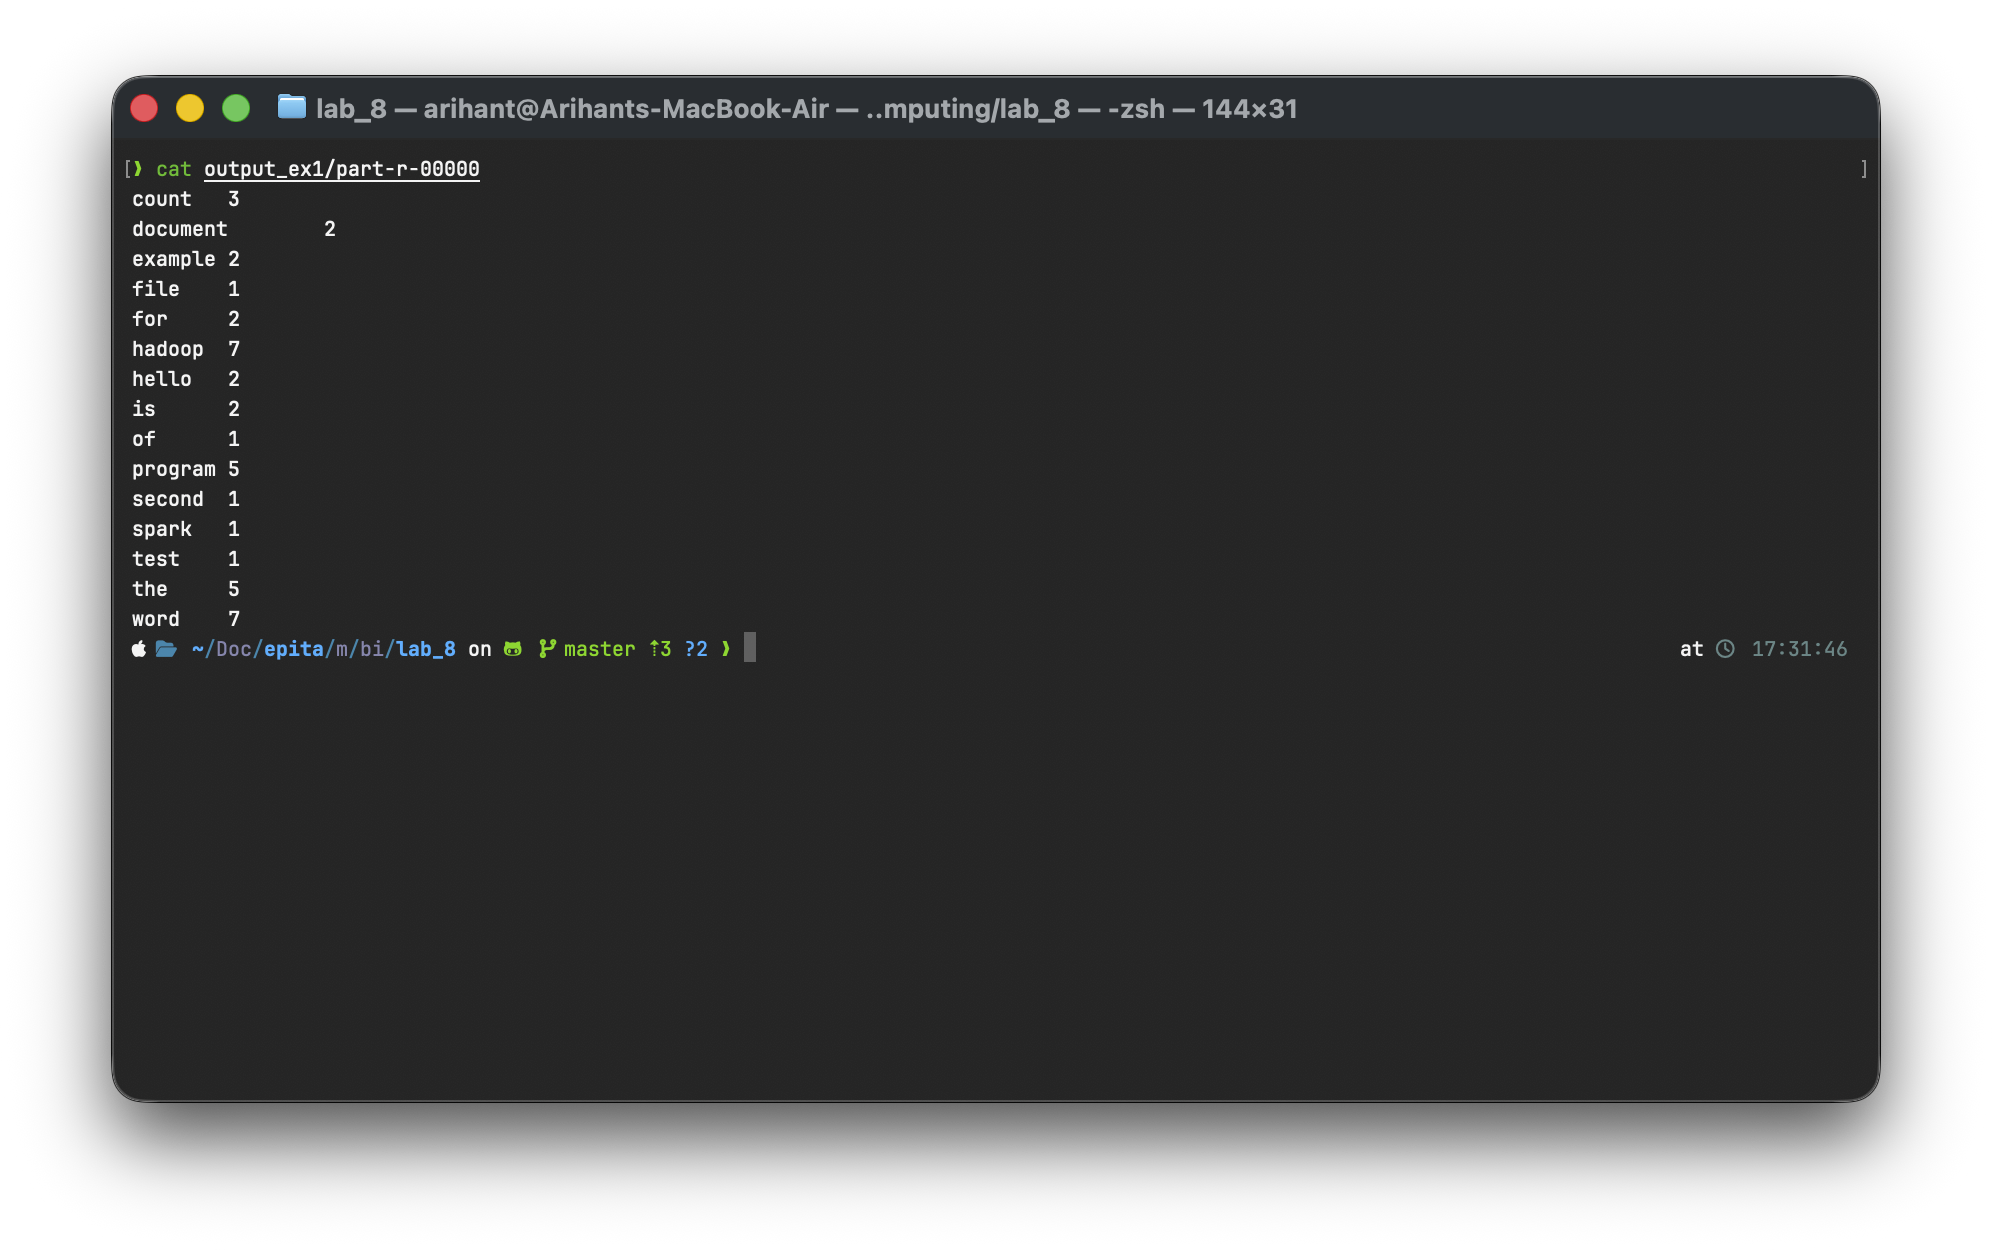
\includegraphics[width=0.75\textwidth]{screenshots/phase1/part-r-0000_ex1.png}
    \caption{Exercise 1 output}
\end{figure}

\section{Word Count (Multiple Files)}

\subsection*{Objective}
Count the occurrences of each word across all files in an input directory.

\subsection*{Implementation}
The same mapper and reducer used in Exercise 1 are reused here. Hadoop reads all files in the input directory and sends their records through the same pipeline.

\subsection*{Result}
The counts are aggregated across the full directory, not only one file.

\section{Word Count with Combiner}

\subsection*{Objective}
Reduce the amount of intermediate data sent to the reducer.

\subsection*{Implementation}
A combiner is used to sum local word counts on each mapper before the shuffle phase. The final reducer still produces the same word count output.

\subsection*{Result}
The final counts remain the same, while the shuffled data is reduced.

\begin{figure}[H]
    \centering
    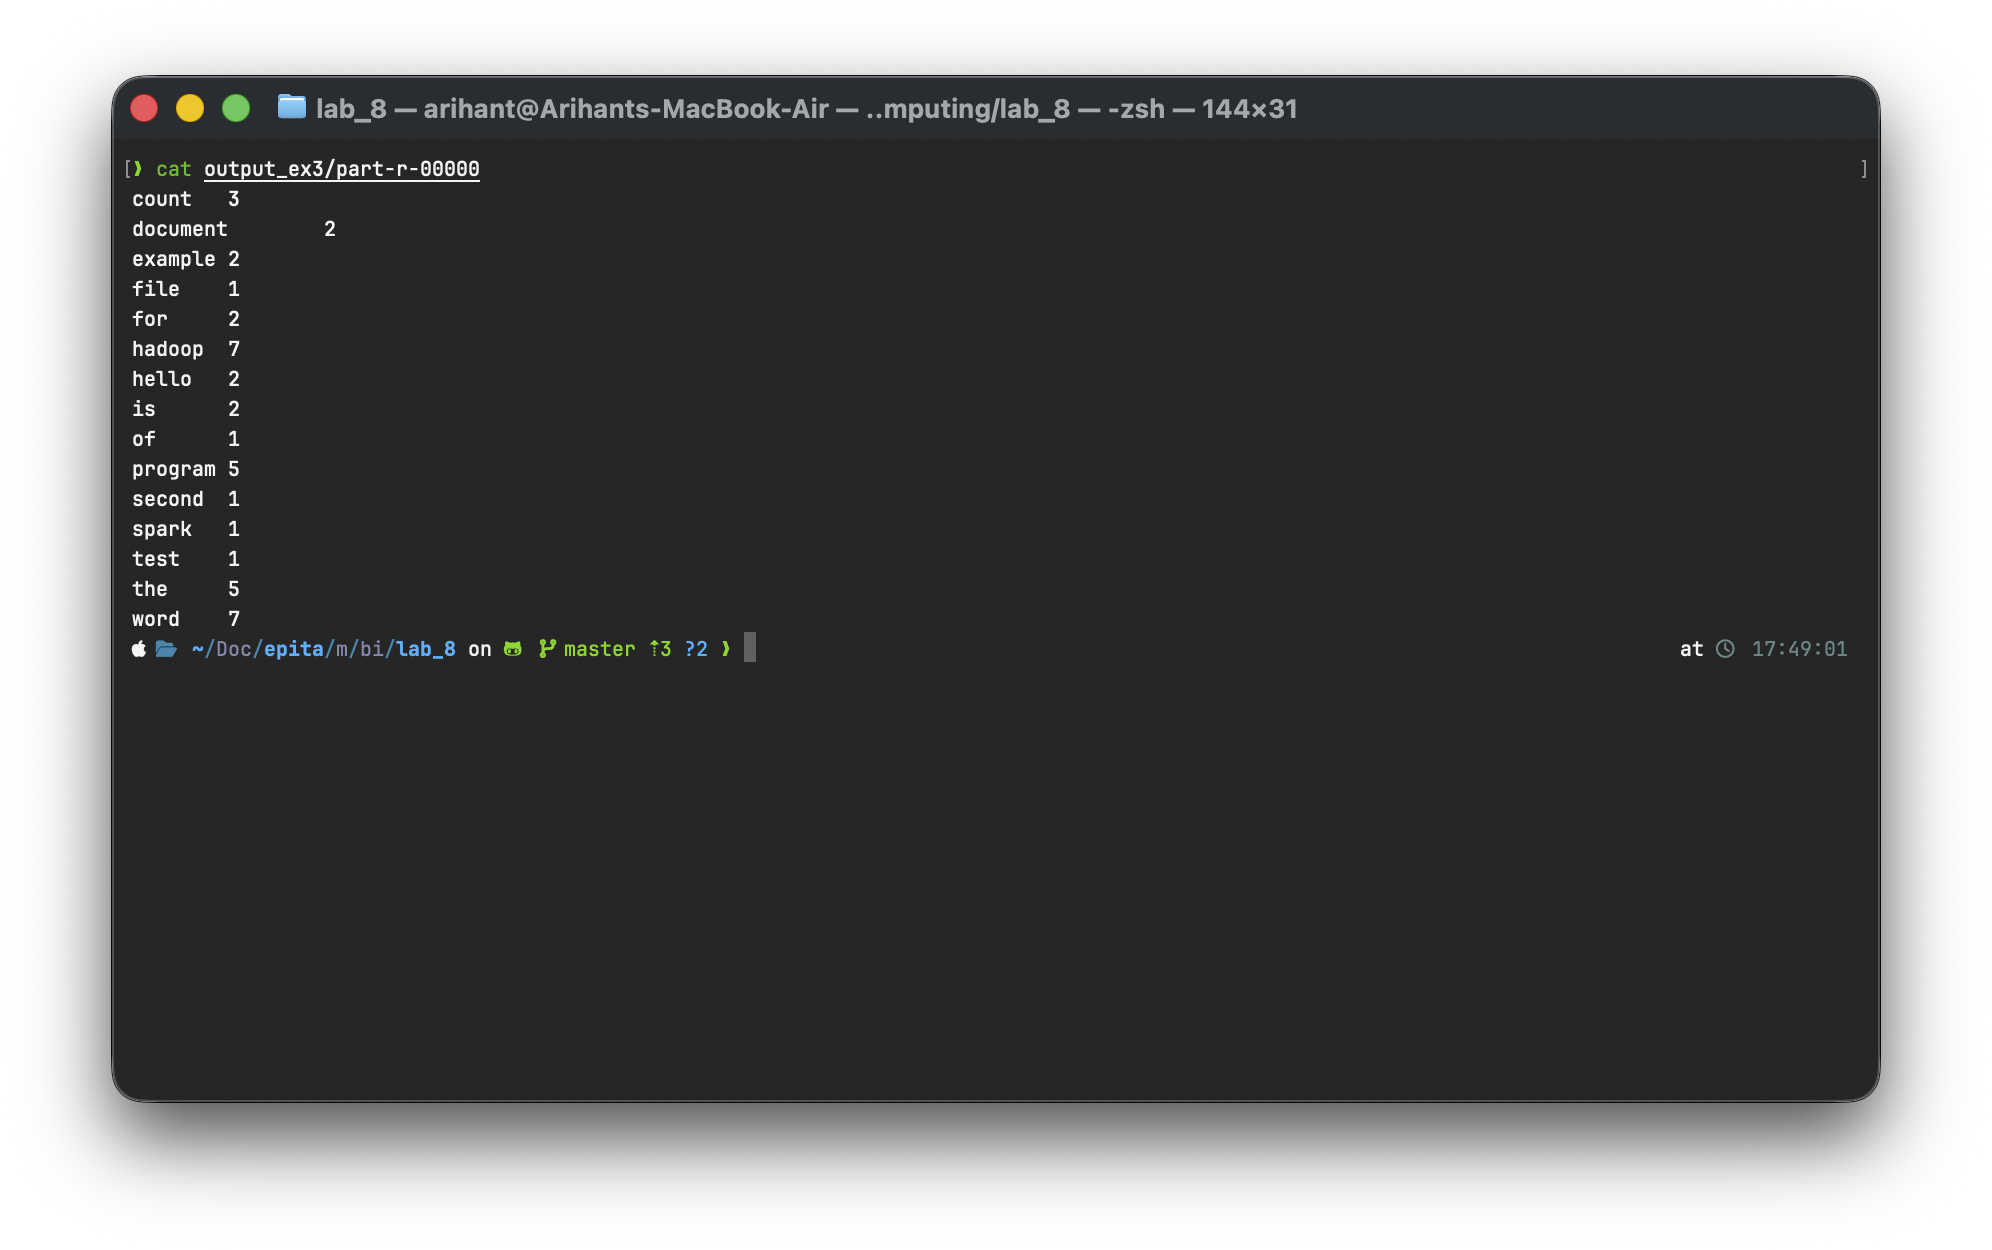
\includegraphics[width=0.75\textwidth]{screenshots/phase1/part-r-0000_ex3.png}
    \caption{Exercise 3 output}
\end{figure}

\section{PM10 Above Threshold}

\subsection*{Objective}
Count, for each sensor, how many readings are above the PM10 threshold.

\subsection*{Implementation}
The mapper filters records above the threshold and emits the sensor identifier. The reducer counts the number of matching records per sensor.

\subsection*{Result}
In the sample data, sensor \texttt{s1} has 2 matches and sensor \texttt{s2} has 1 match.

\begin{figure}[H]
    \centering
    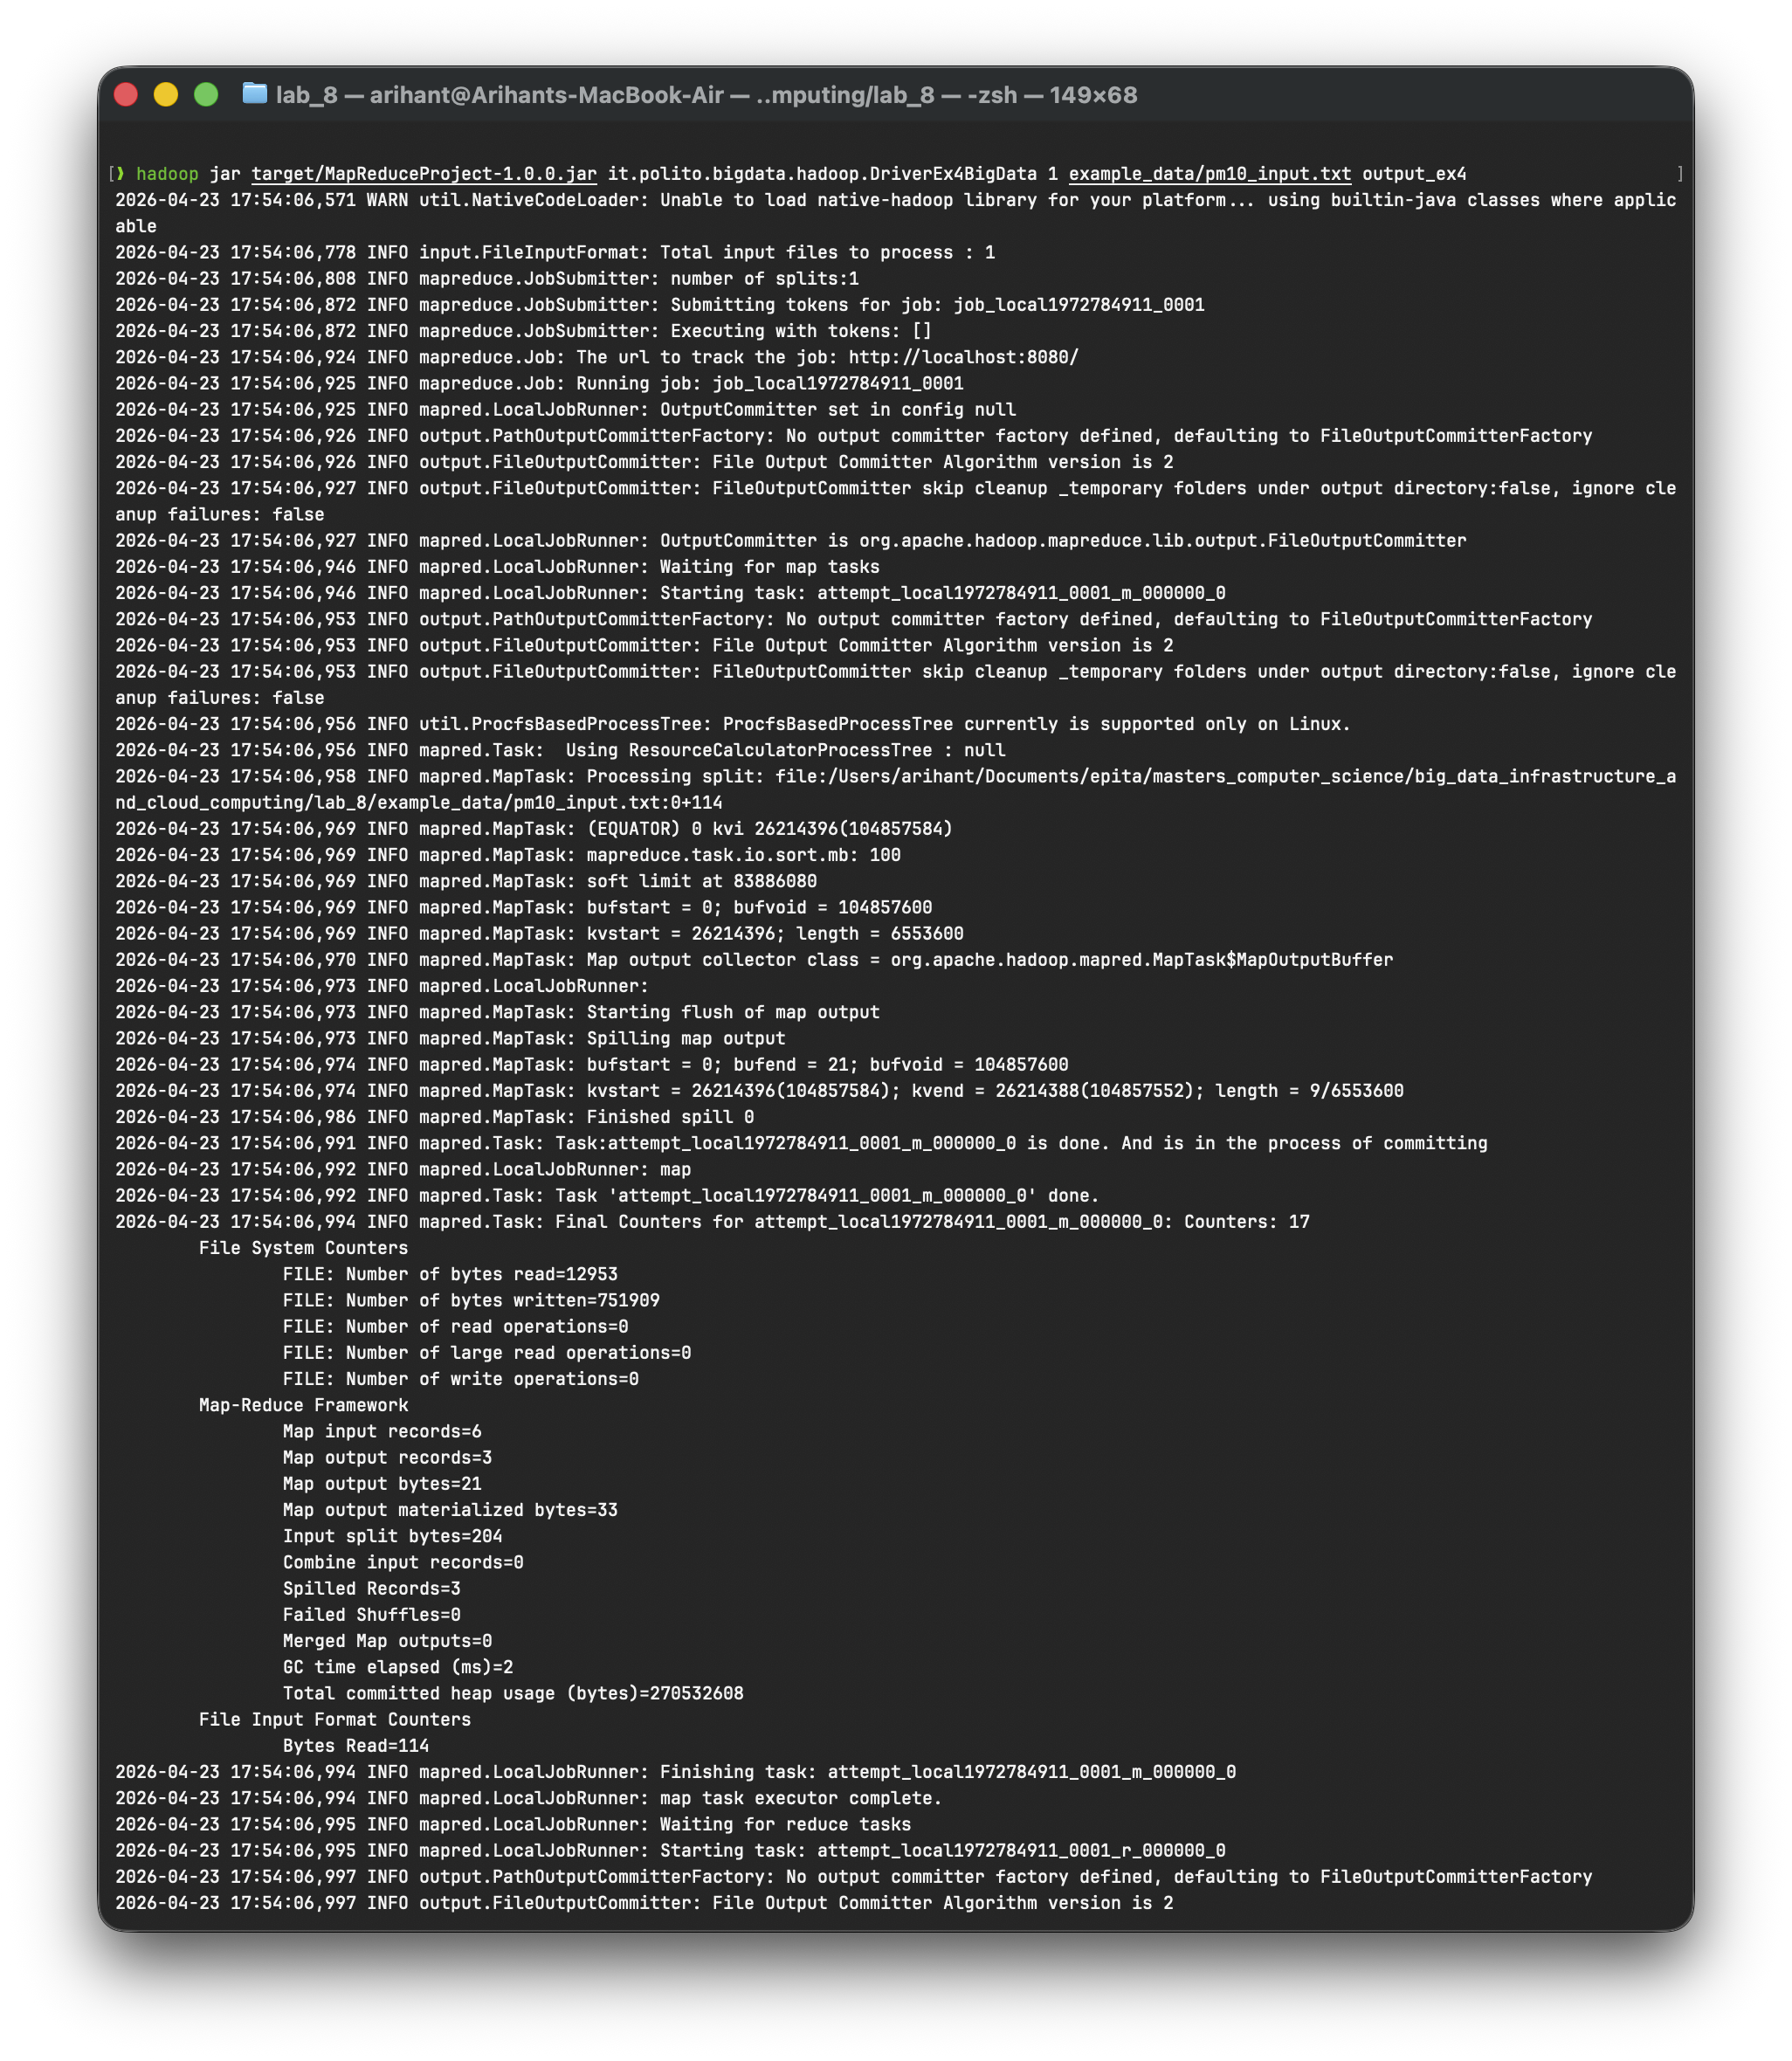
\includegraphics[width=0.75\textwidth]{screenshots/phase2/hadoop_cmd_ex4.png}
    \caption{Exercise 4 command}
\end{figure}

\begin{figure}[H]
    \centering
    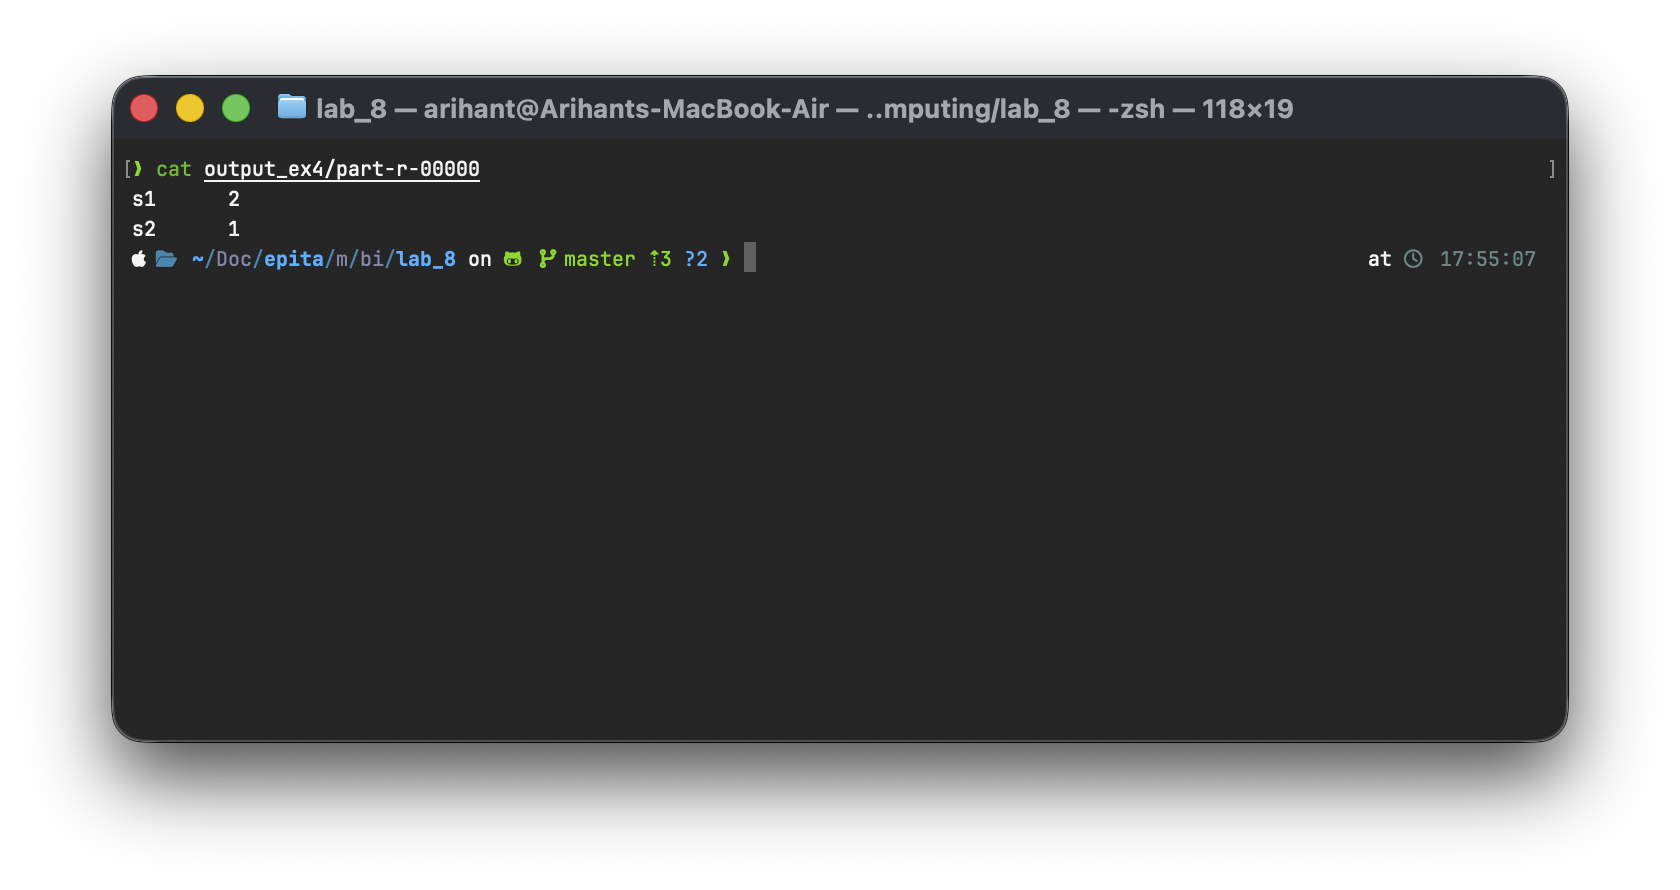
\includegraphics[width=0.75\textwidth]{screenshots/phase2/part-r-0000_ex4.png}
    \caption{Exercise 4 output}
\end{figure}

\section{PM10 per Zone}

\subsection*{Objective}
List the dates where PM10 is above the threshold for each zone.

\subsection*{Implementation}
The mapper emits the zone and date for records that pass the threshold. The reducer groups the dates for each zone.

\subsection*{Result}
The output shows, for each zone, the dates where the threshold was exceeded.

\begin{figure}[H]
    \centering
    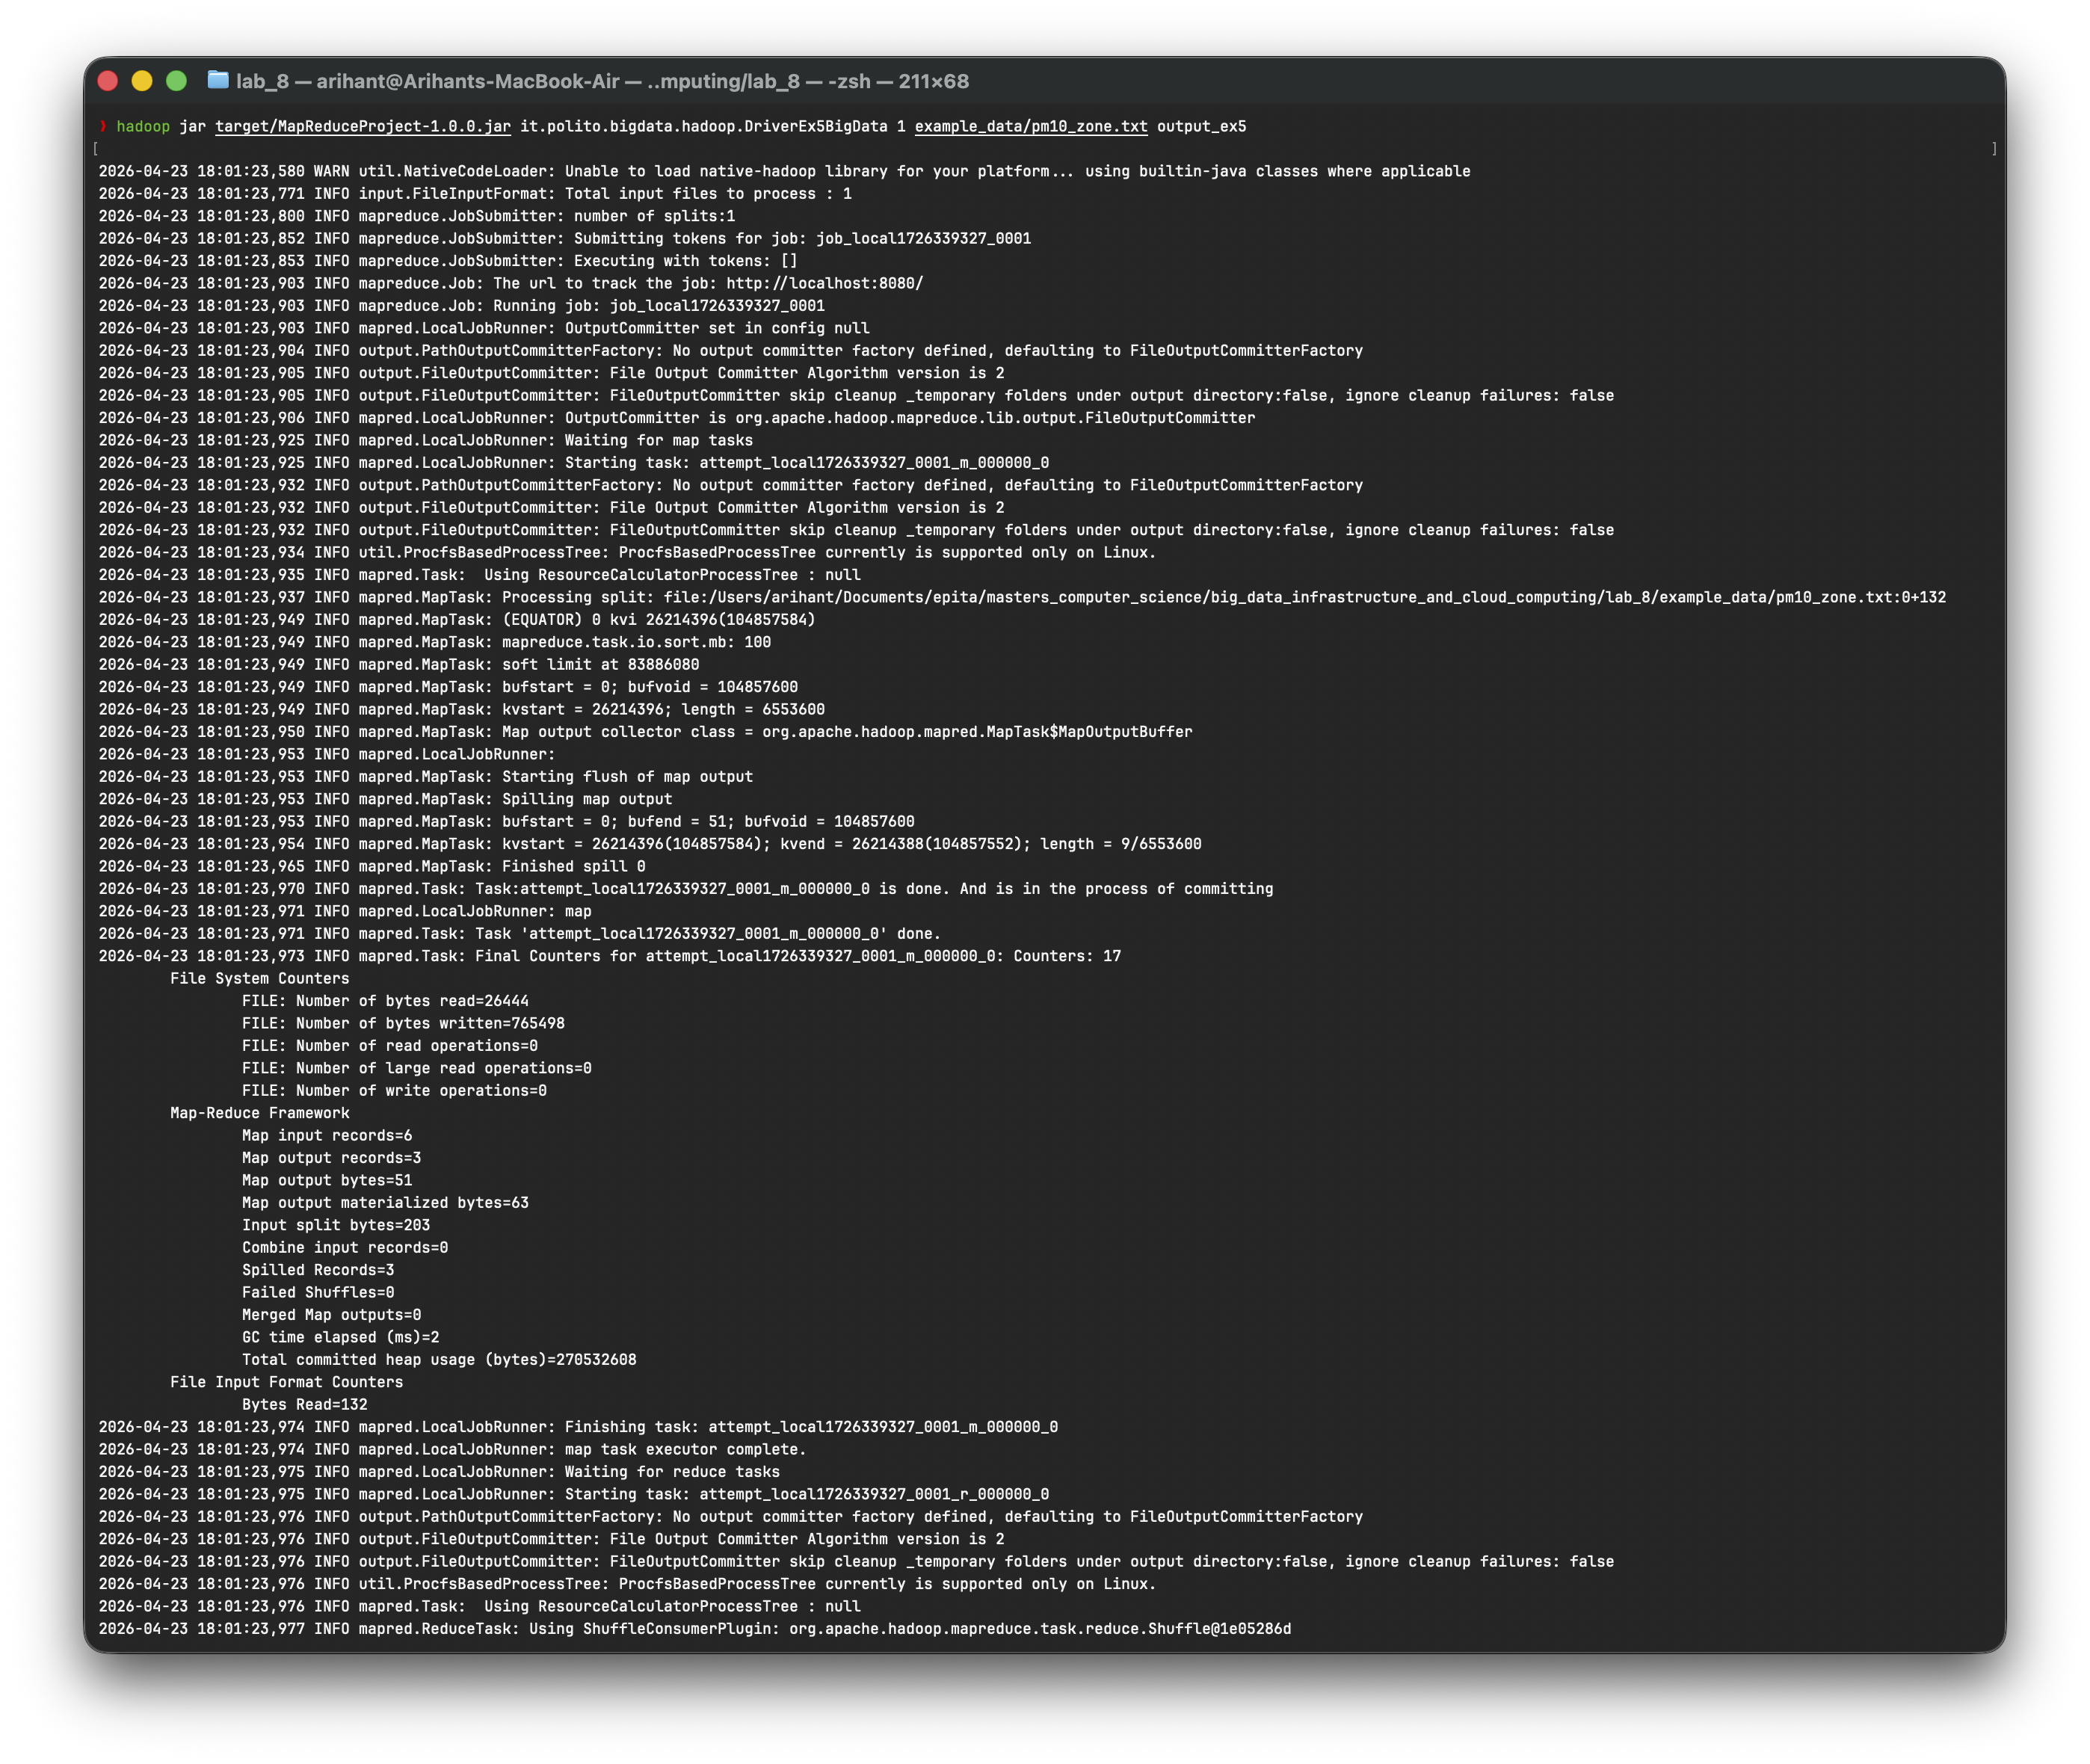
\includegraphics[width=0.75\textwidth]{screenshots/phase2/hadoop_cmd_ex5.png}
    \caption{Exercise 5 command}
\end{figure}

\begin{figure}[H]
    \centering
    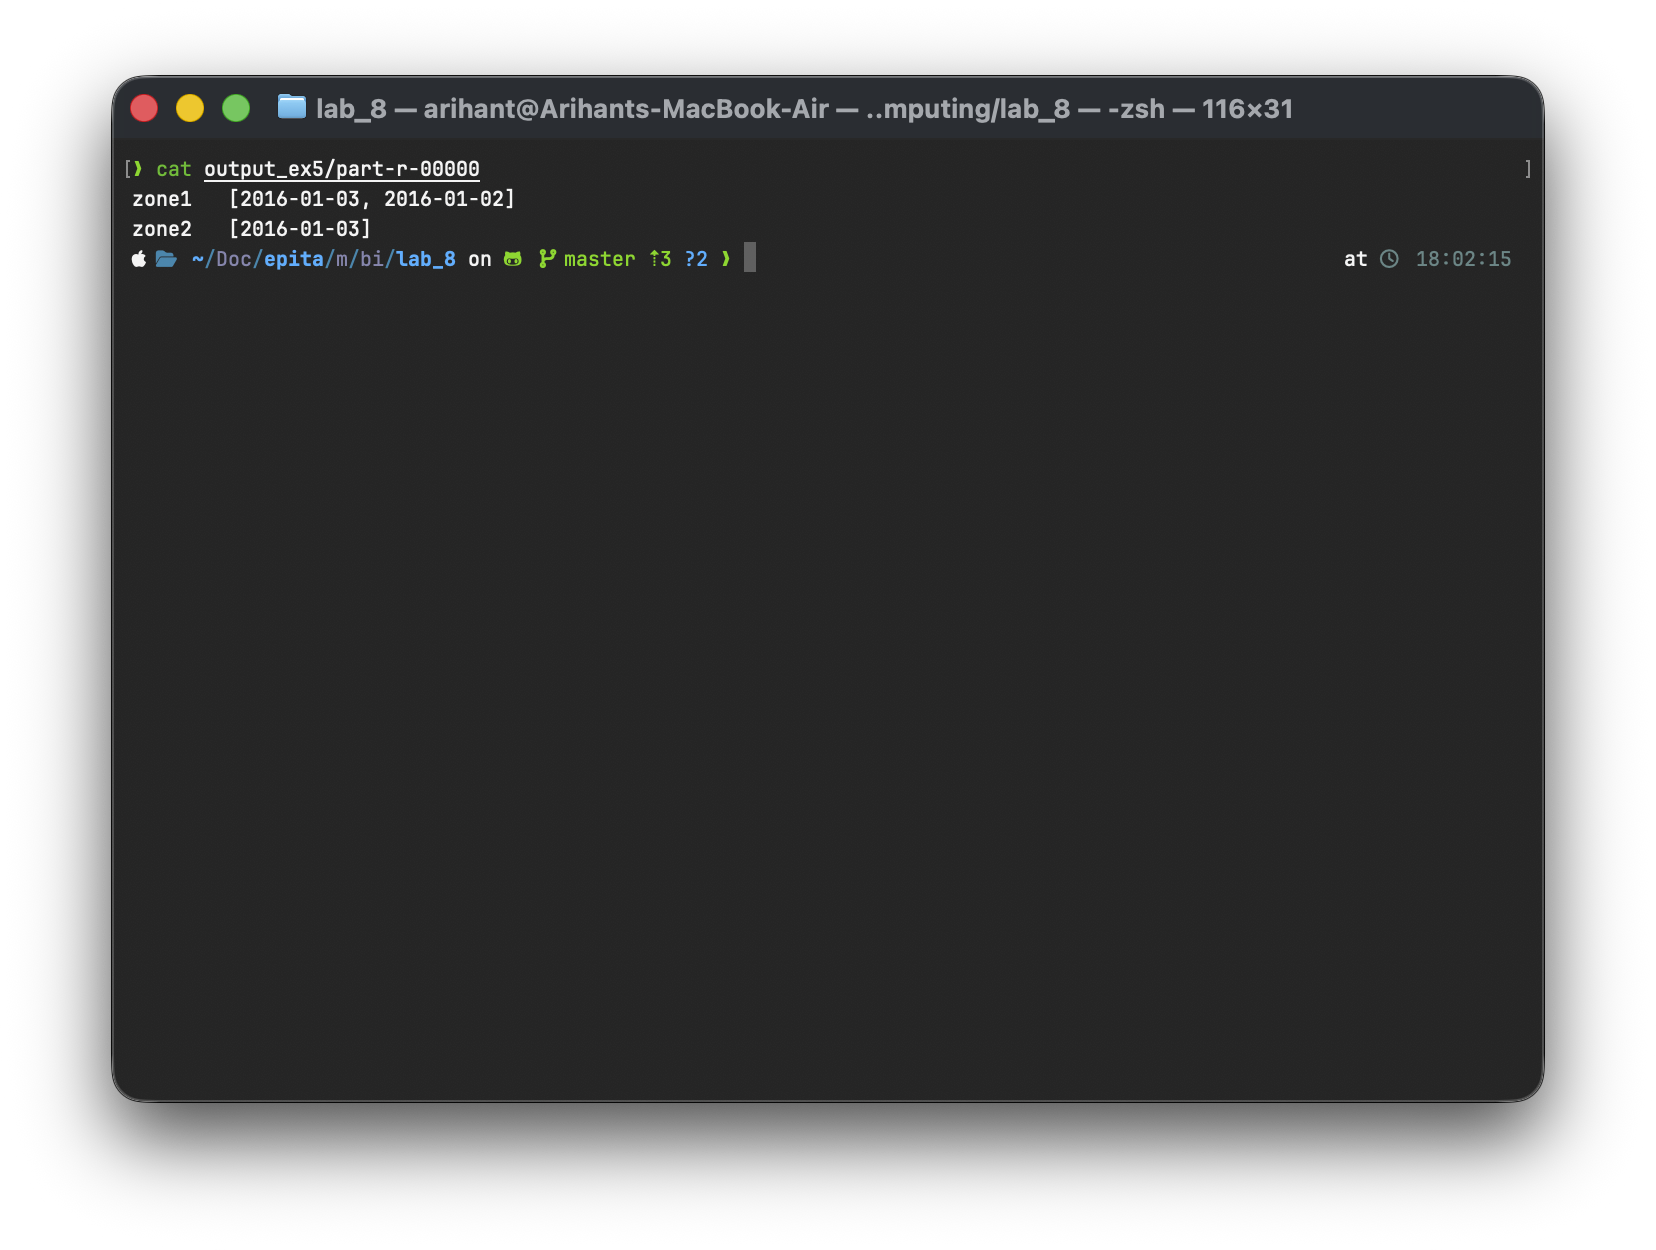
\includegraphics[width=0.75\textwidth]{screenshots/phase2/part-r-0000_ex5.png}
    \caption{Exercise 5 output}
\end{figure}

\section{Average PM10}

\subsection*{Objective}
Compute the average PM10 value for each sensor.

\subsection*{Implementation}
The mapper emits the sensor and the PM10 value. The reducer computes the sum and count, then writes the average.

\subsection*{Result}
The sample output gives \texttt{s1 = 45.4} and \texttt{s2 = 34.3}.

\begin{figure}[H]
    \centering
    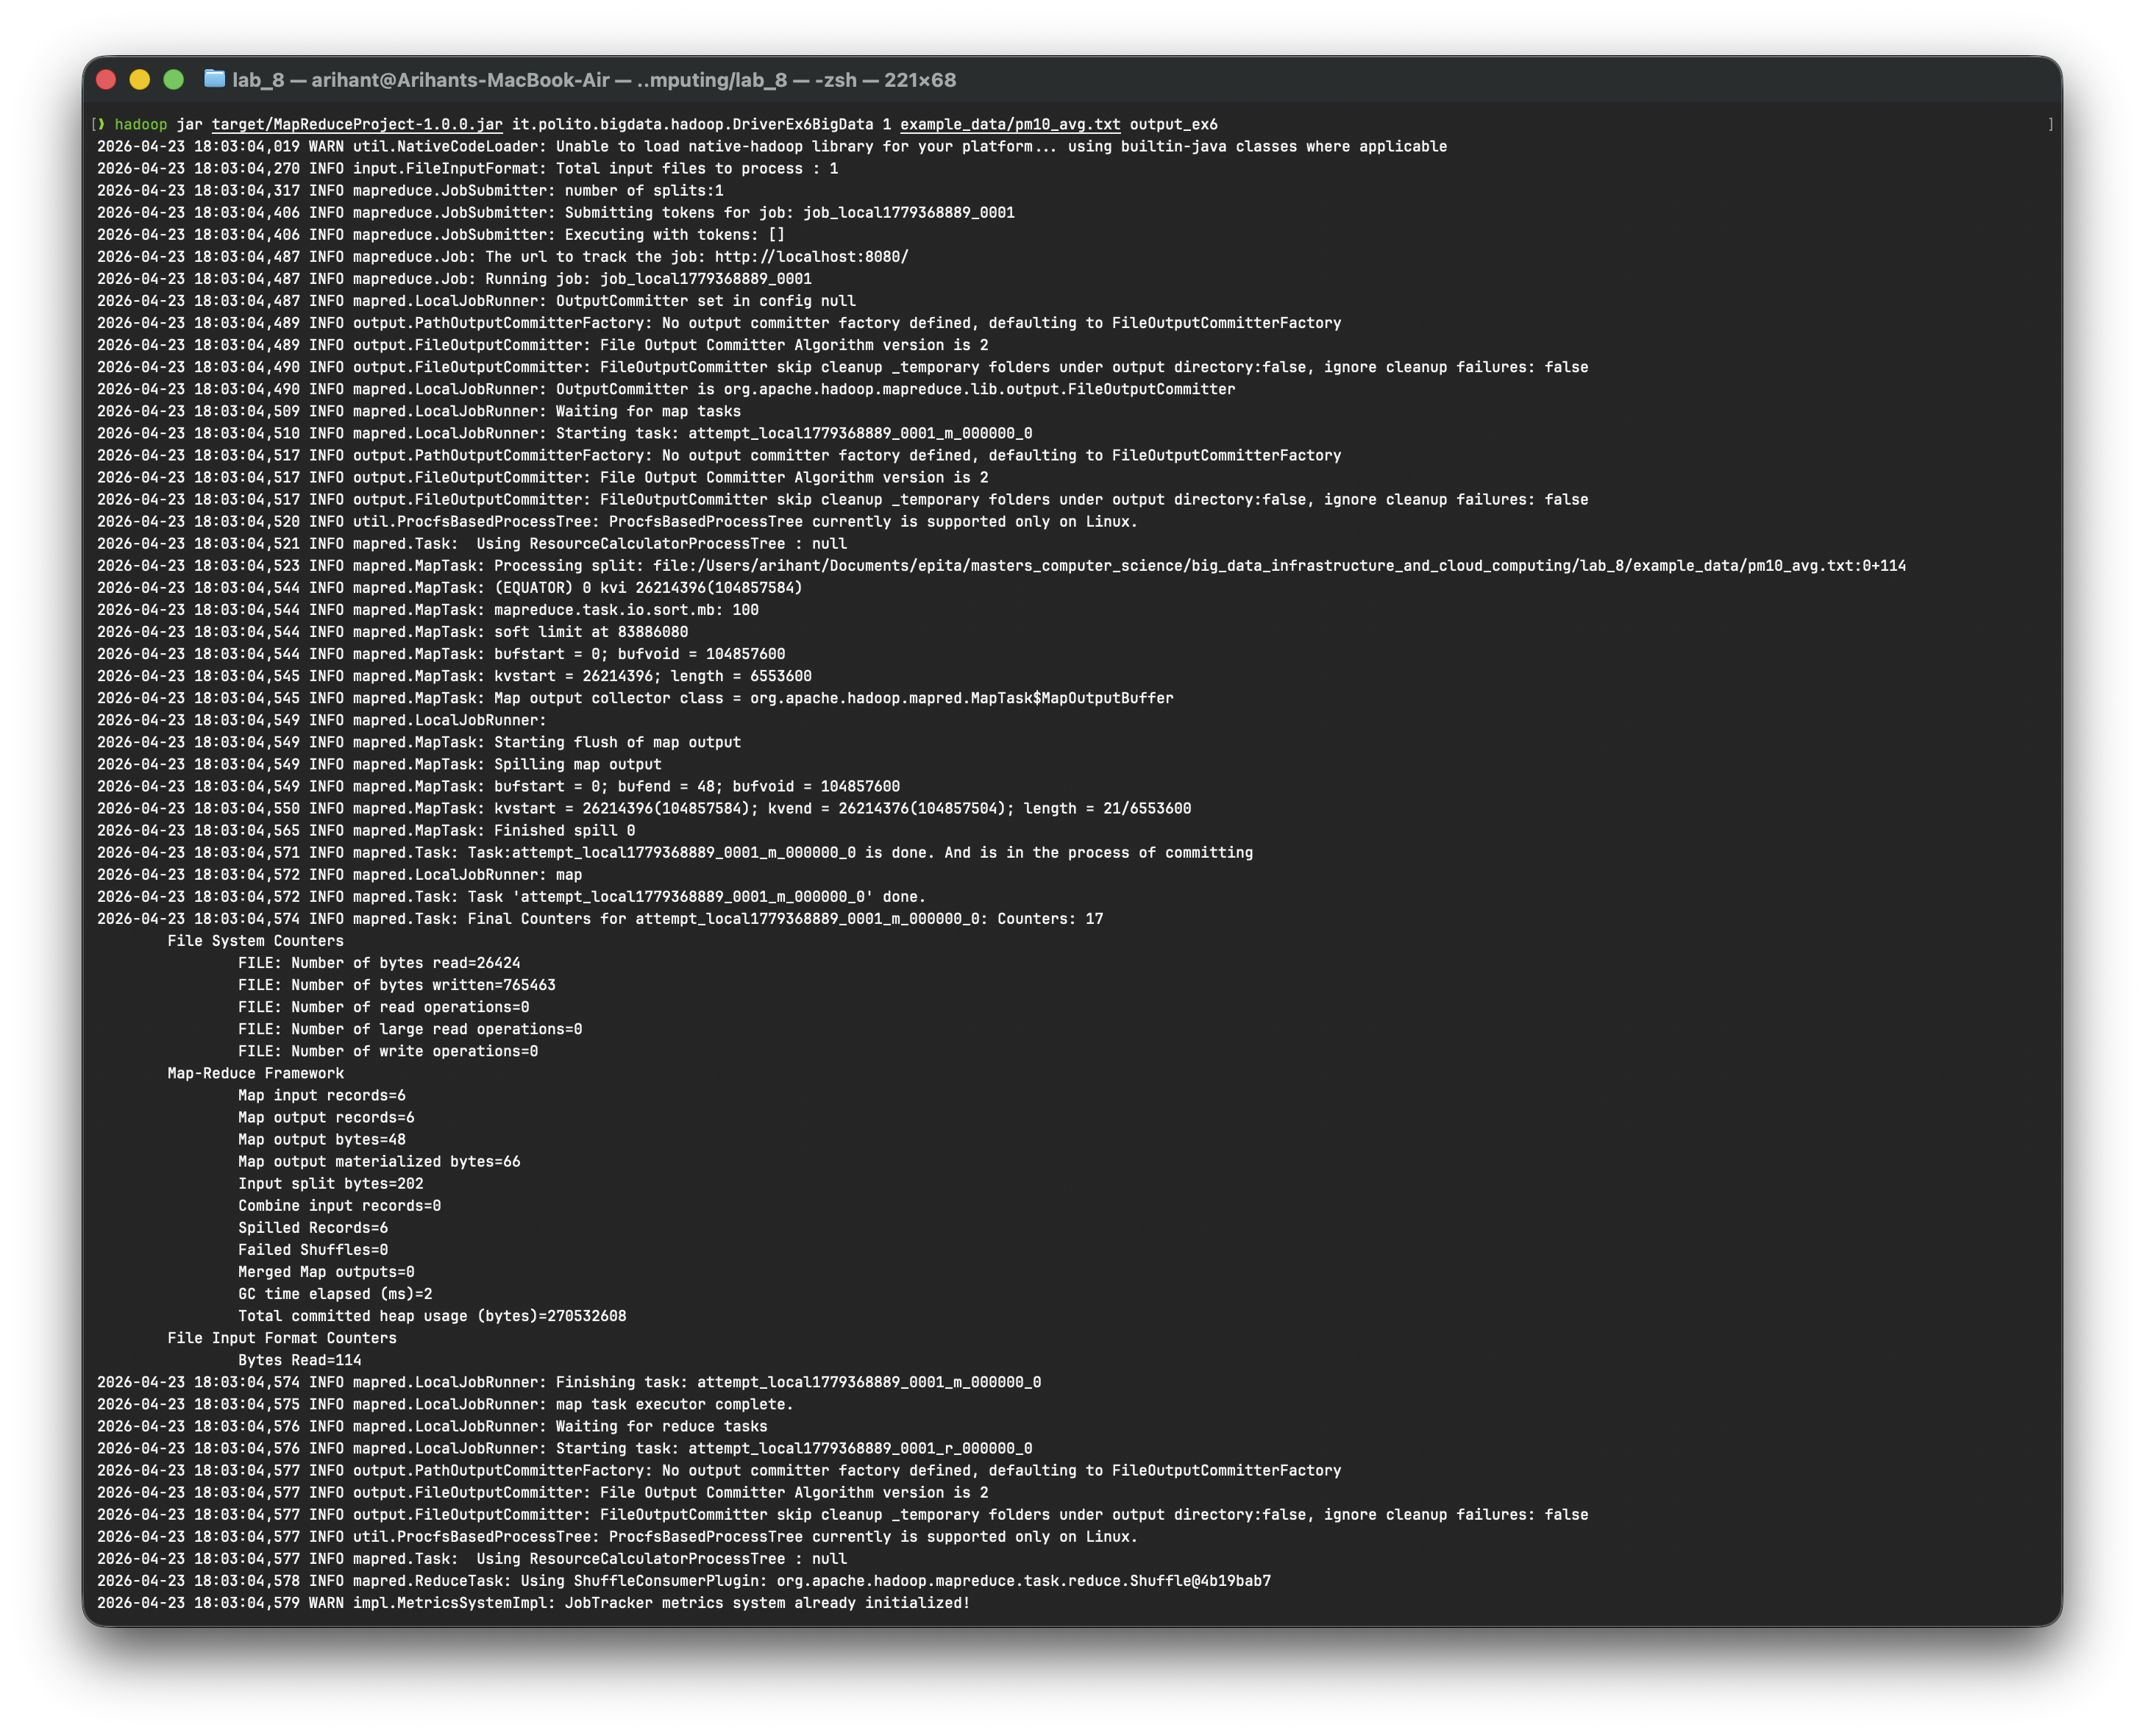
\includegraphics[width=0.75\textwidth]{screenshots/phase2/hadoop_cmd_ex6.png}
    \caption{Exercise 6 command}
\end{figure}

\begin{figure}[H]
    \centering
    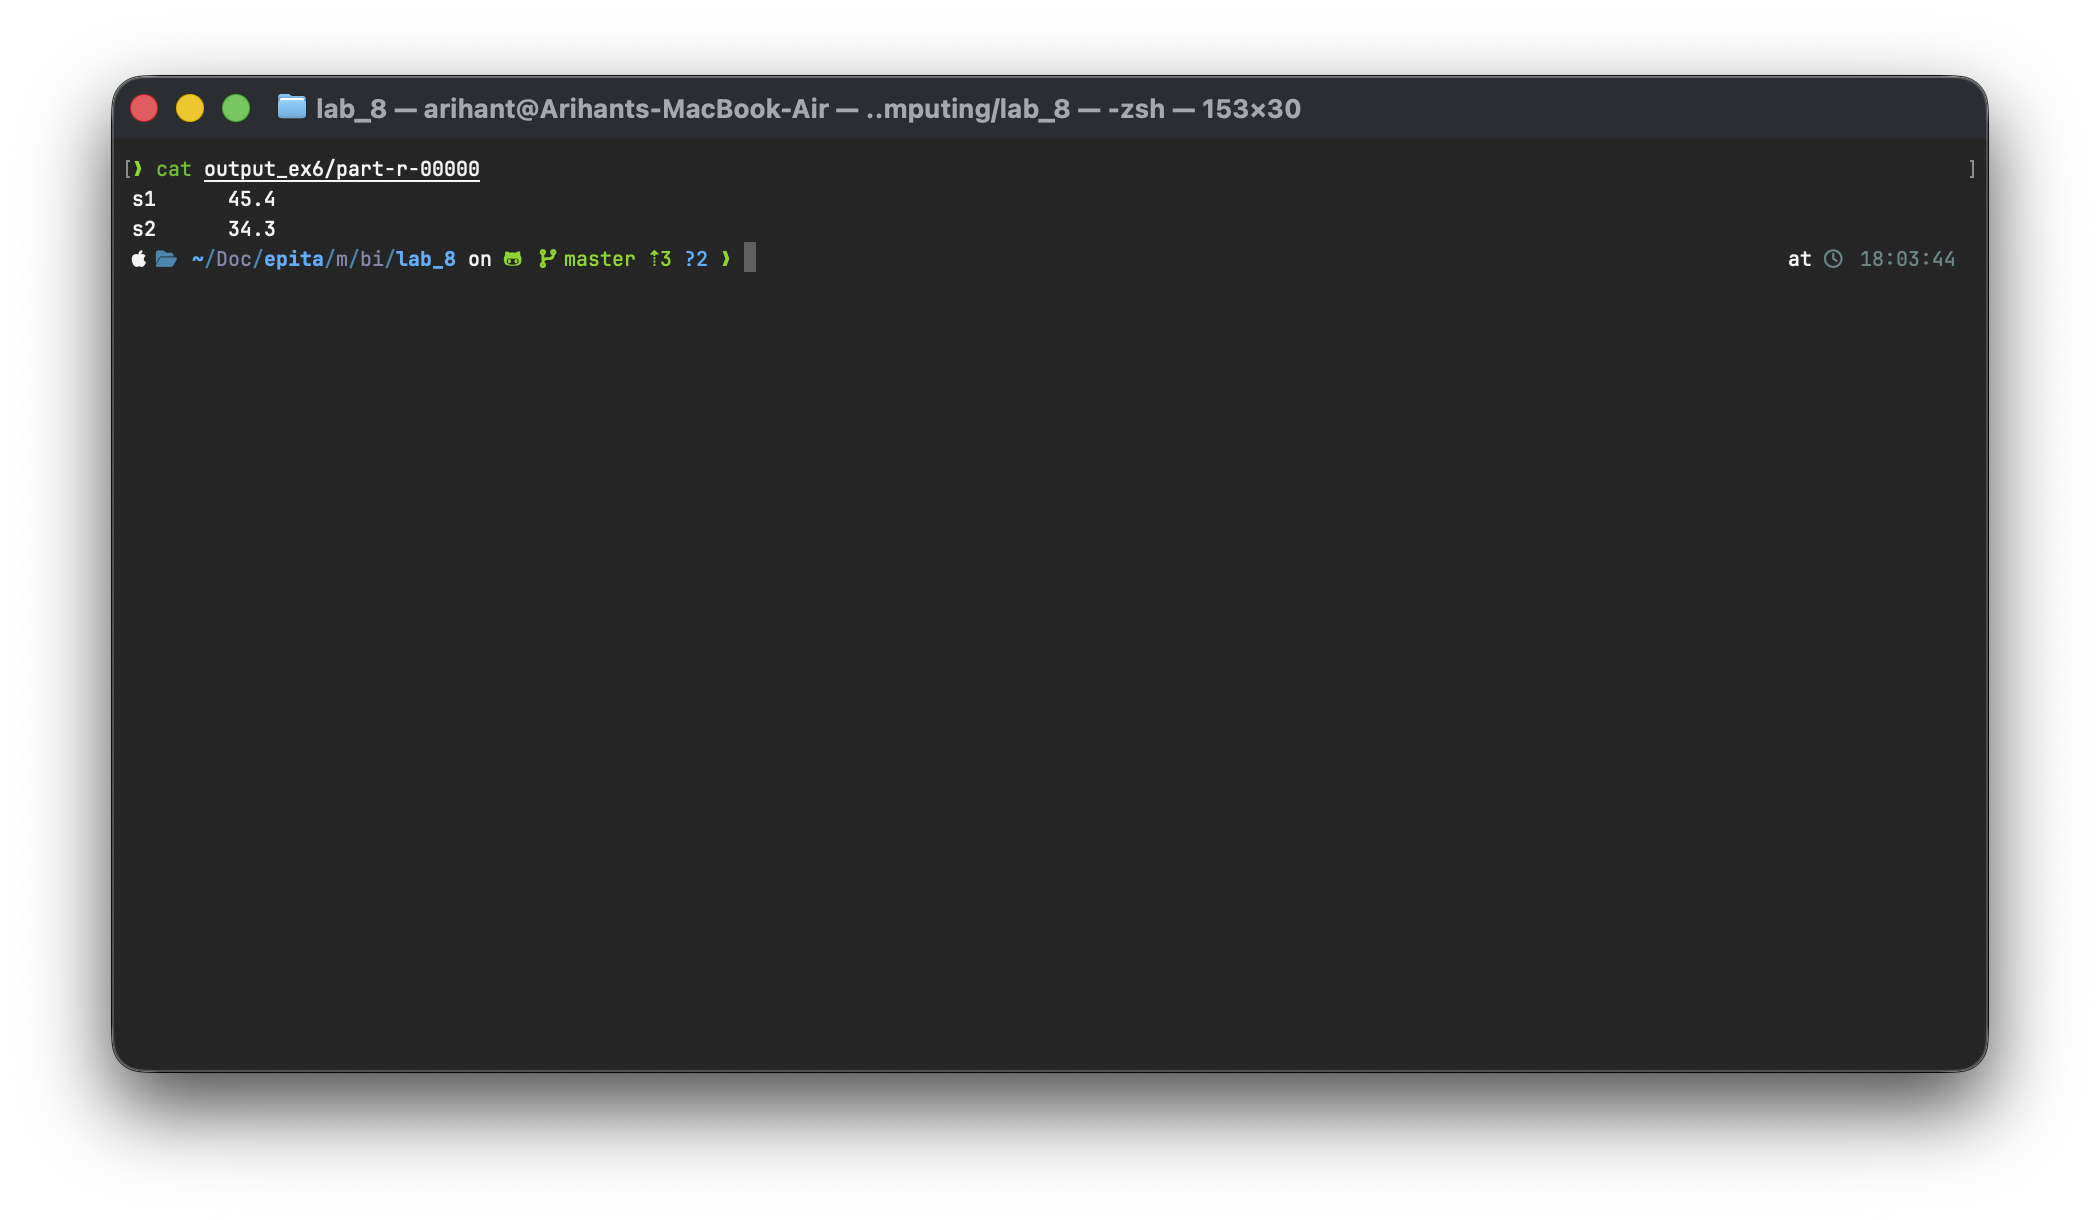
\includegraphics[width=0.75\textwidth]{screenshots/phase2/part-r-0000_ex6.png}
    \caption{Exercise 6 output}
\end{figure}

\section{Max and Min PM10}

\subsection*{Objective}
Report the maximum and minimum PM10 values for each sensor.

\subsection*{Implementation}
The mapper emits the sensor and the reading value. The reducer keeps track of the largest and smallest values seen for each sensor.

\subsection*{Result}
The output contains the max and min values for each sensor in the sample data.

\begin{figure}[H]
    \centering
    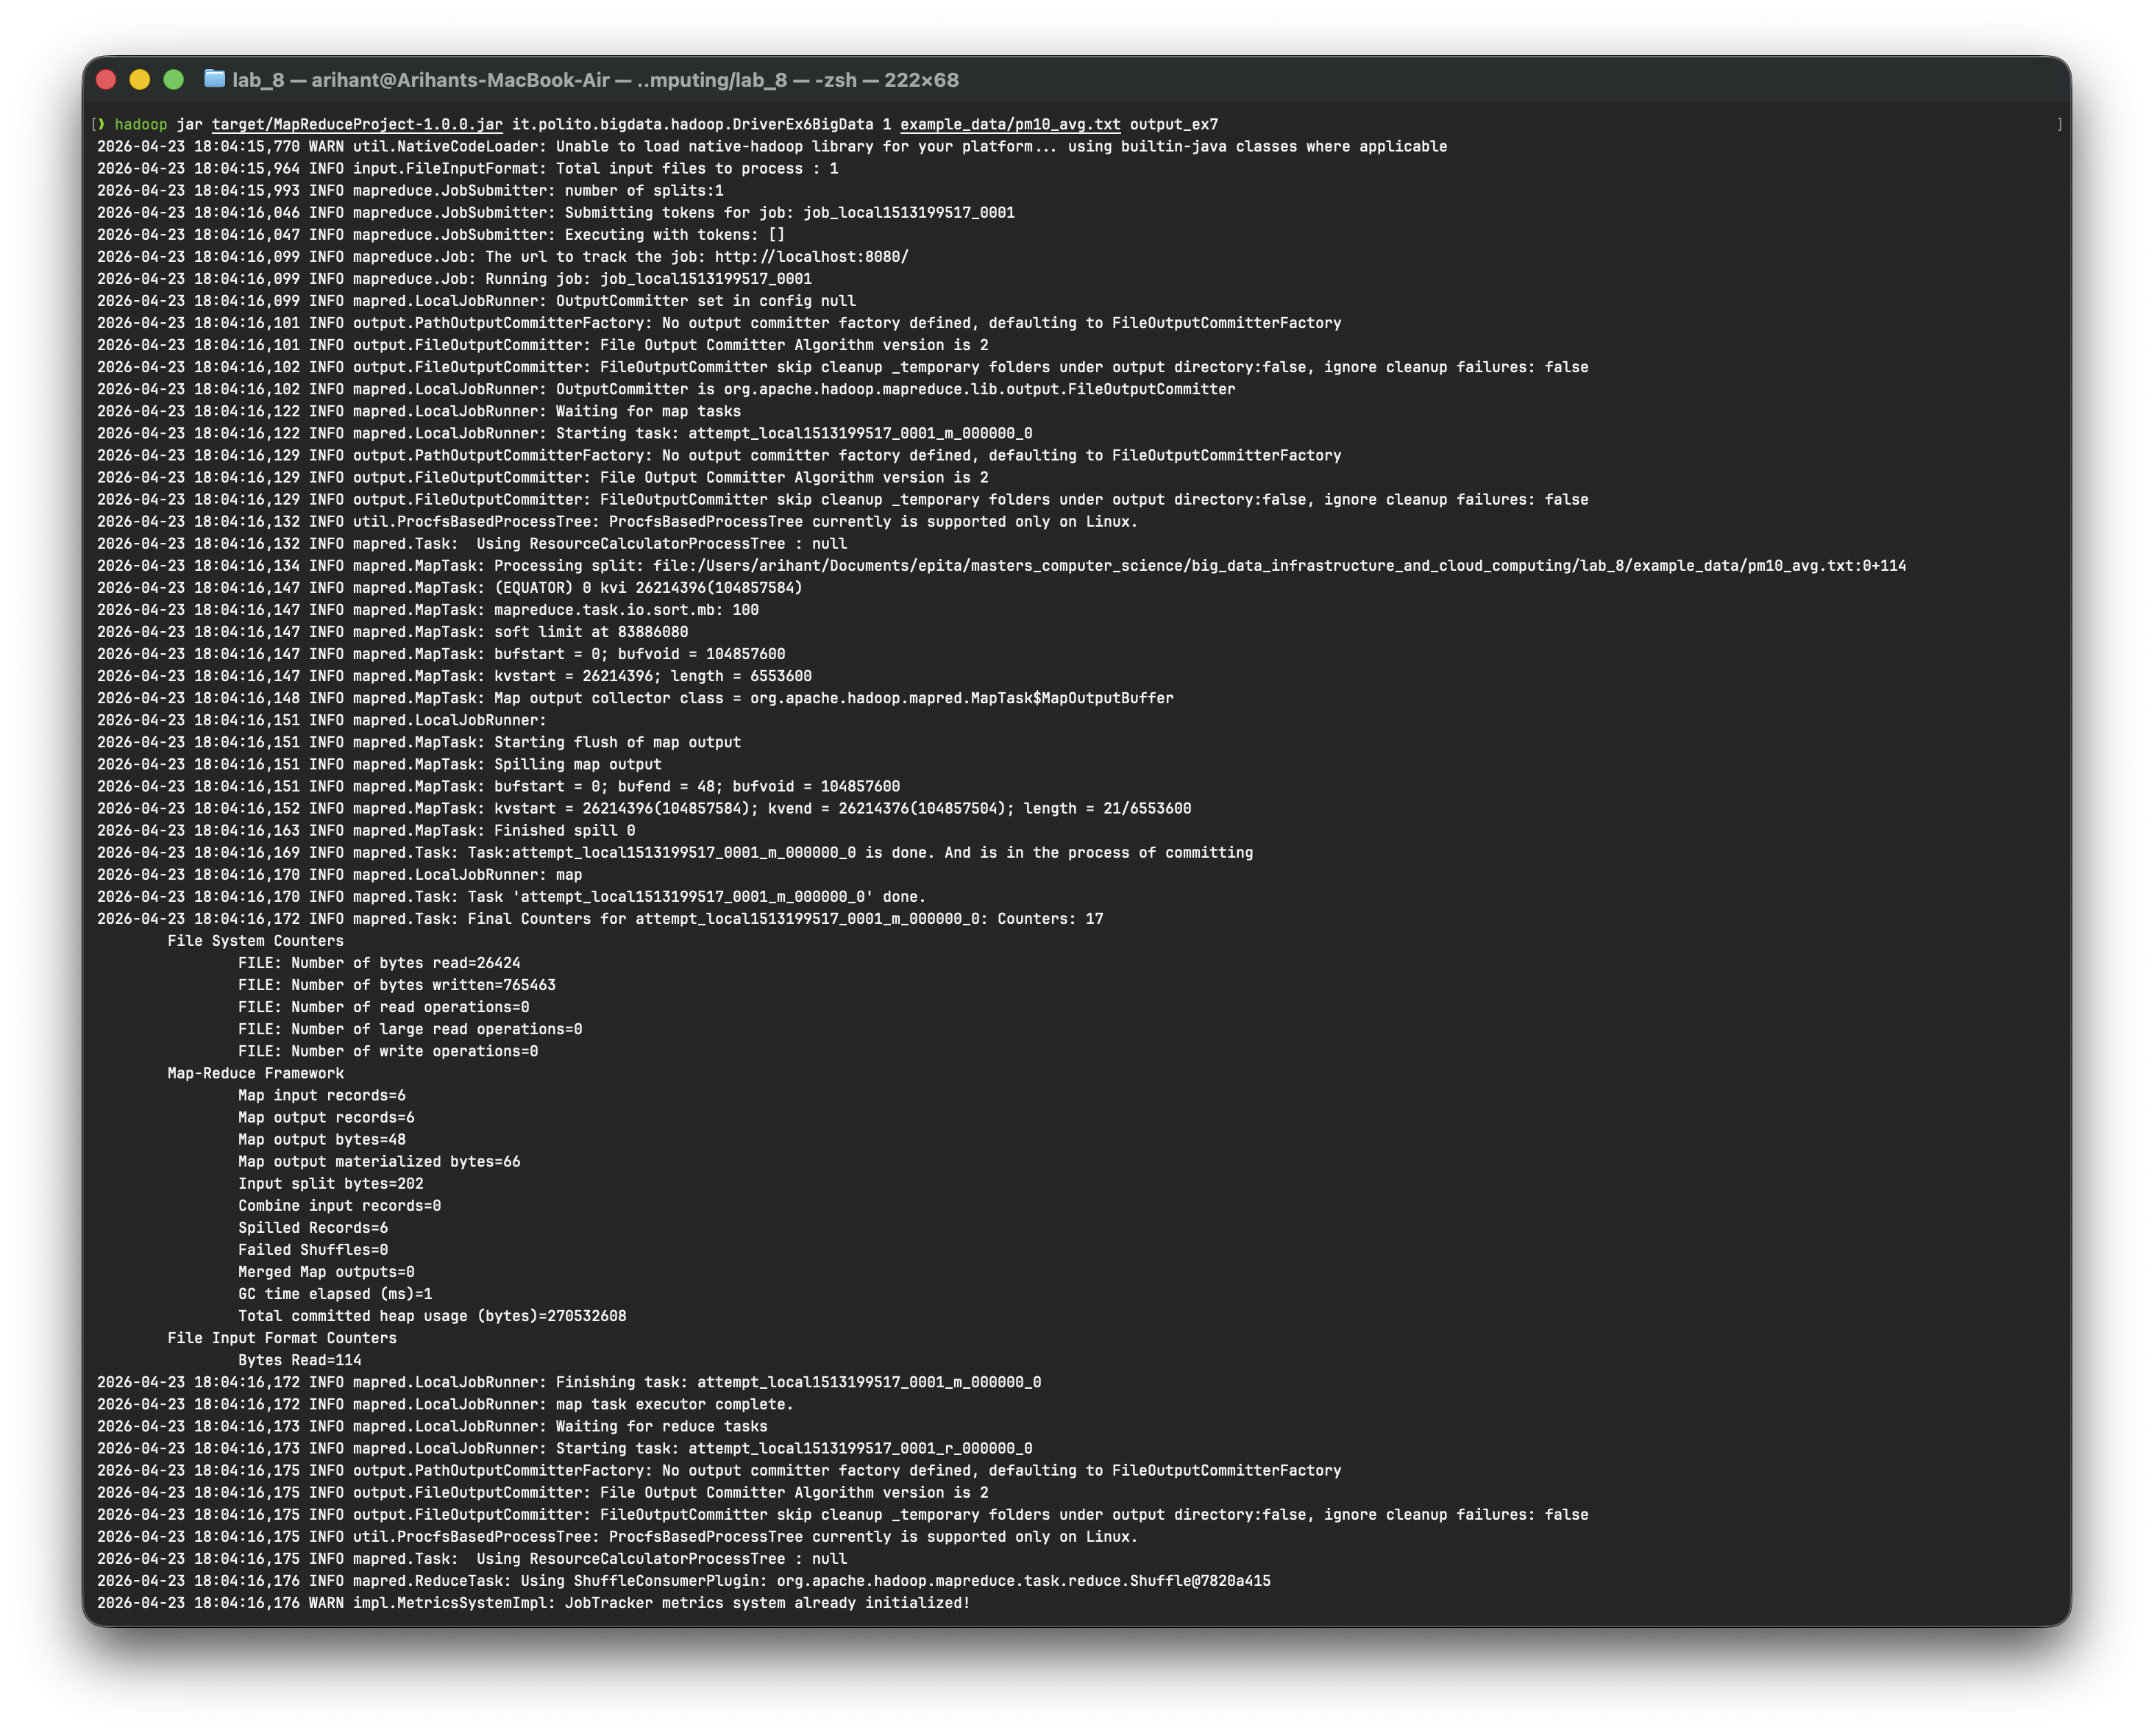
\includegraphics[width=0.75\textwidth]{screenshots/phase2/hadoop_cmd_ex7.png}
    \caption{Exercise 7 command}
\end{figure}

\begin{figure}[H]
    \centering
    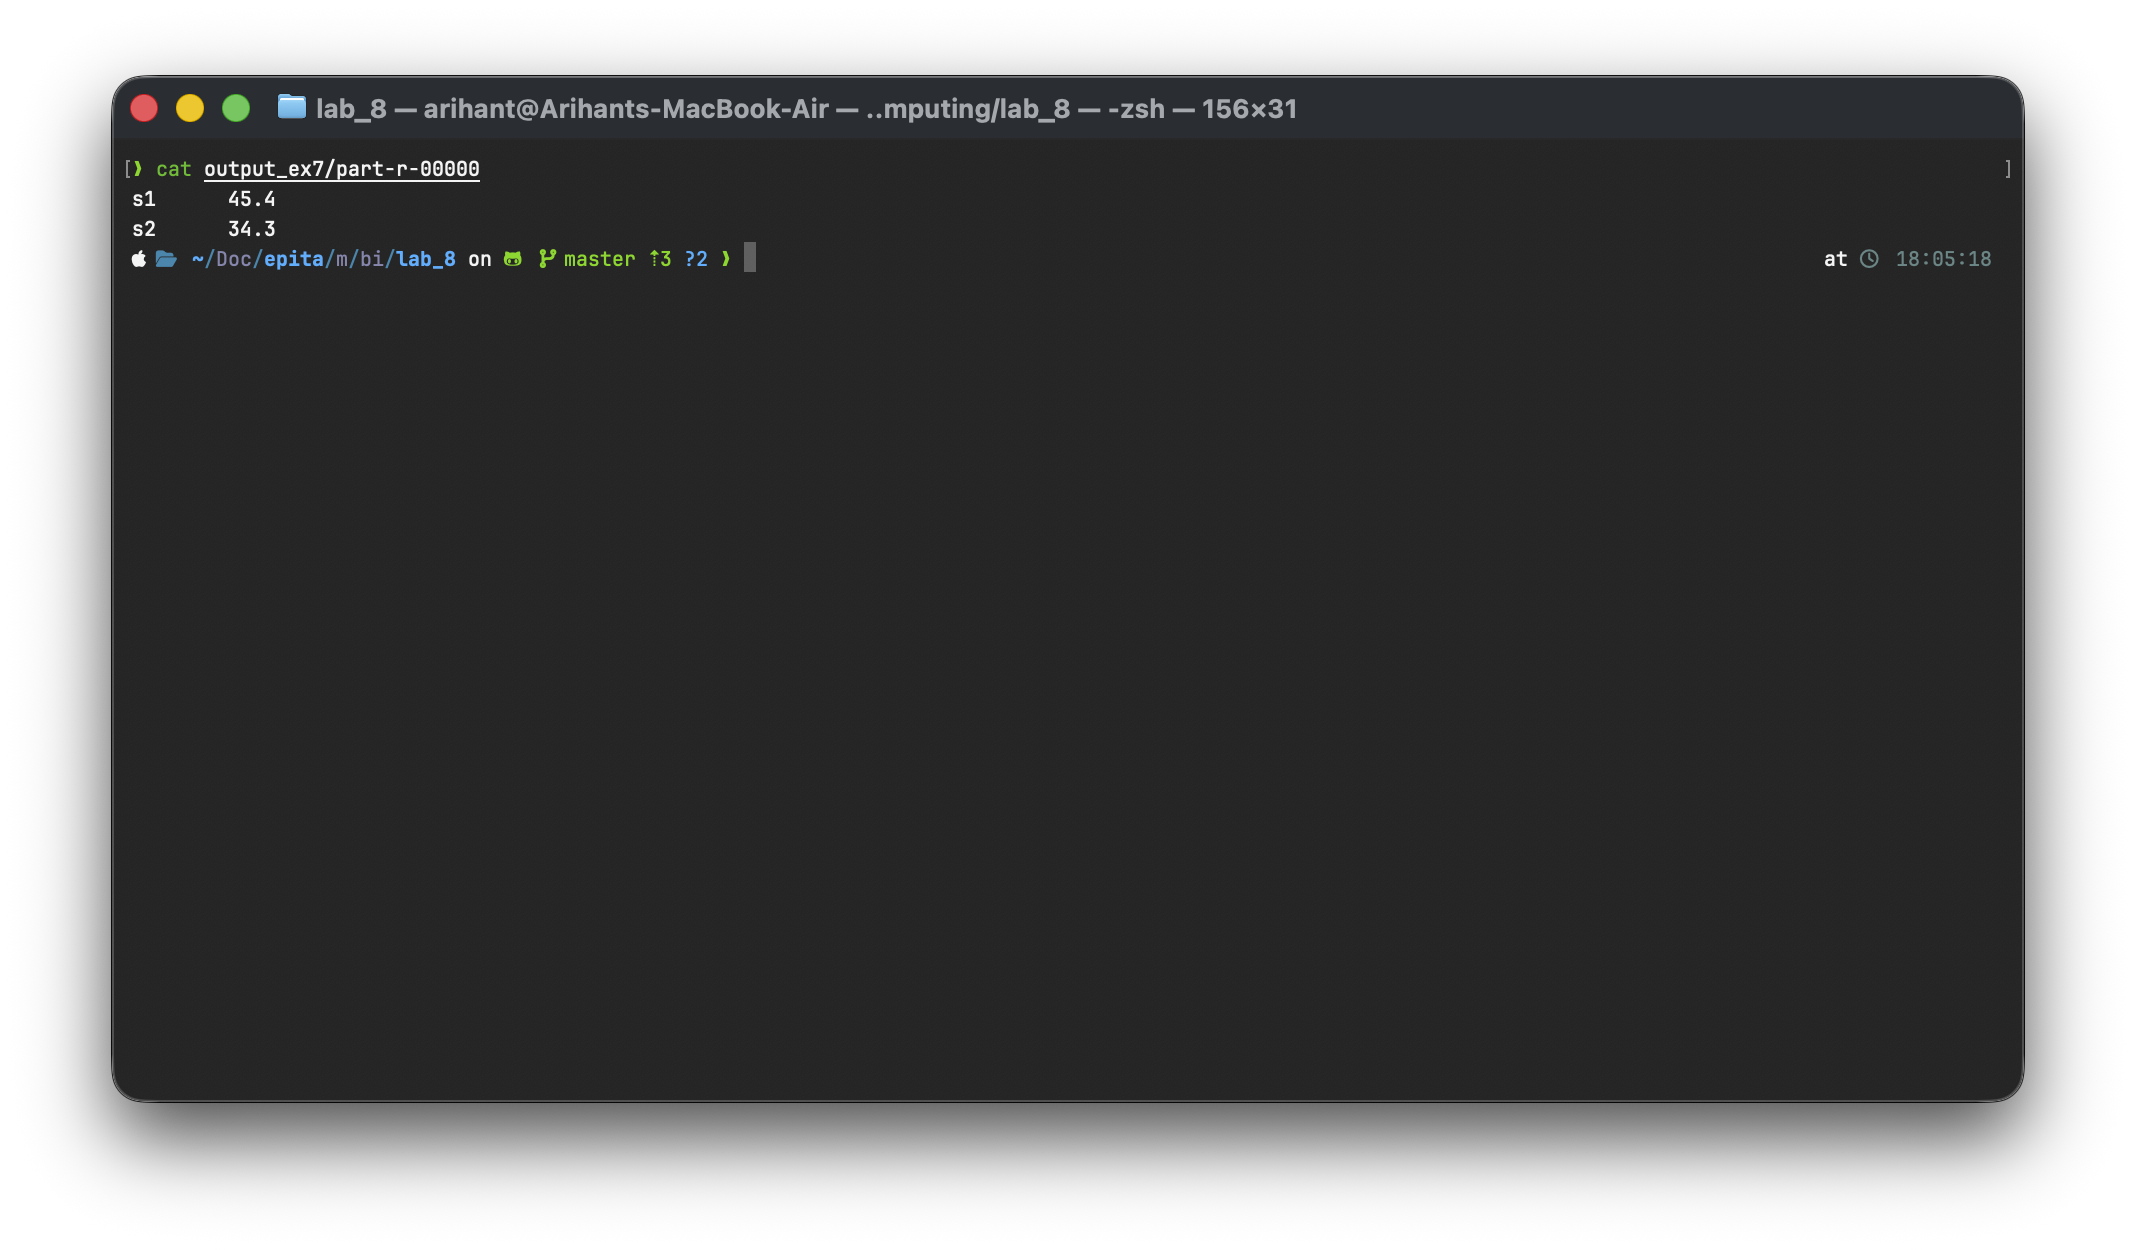
\includegraphics[width=0.75\textwidth]{screenshots/phase2/part-r-0000_ex7.png}
    \caption{Exercise 7 output}
\end{figure}

\section{Total Count}

\subsection*{Objective}
Count the total number of records in the input file.

\subsection*{Implementation}
The mapper emits a fixed key with value \texttt{1} for each record. The reducer sums all emitted values.

\subsection*{Result}
The sample input contains 6 records, so the total count is 6.

\begin{figure}[H]
    \centering
    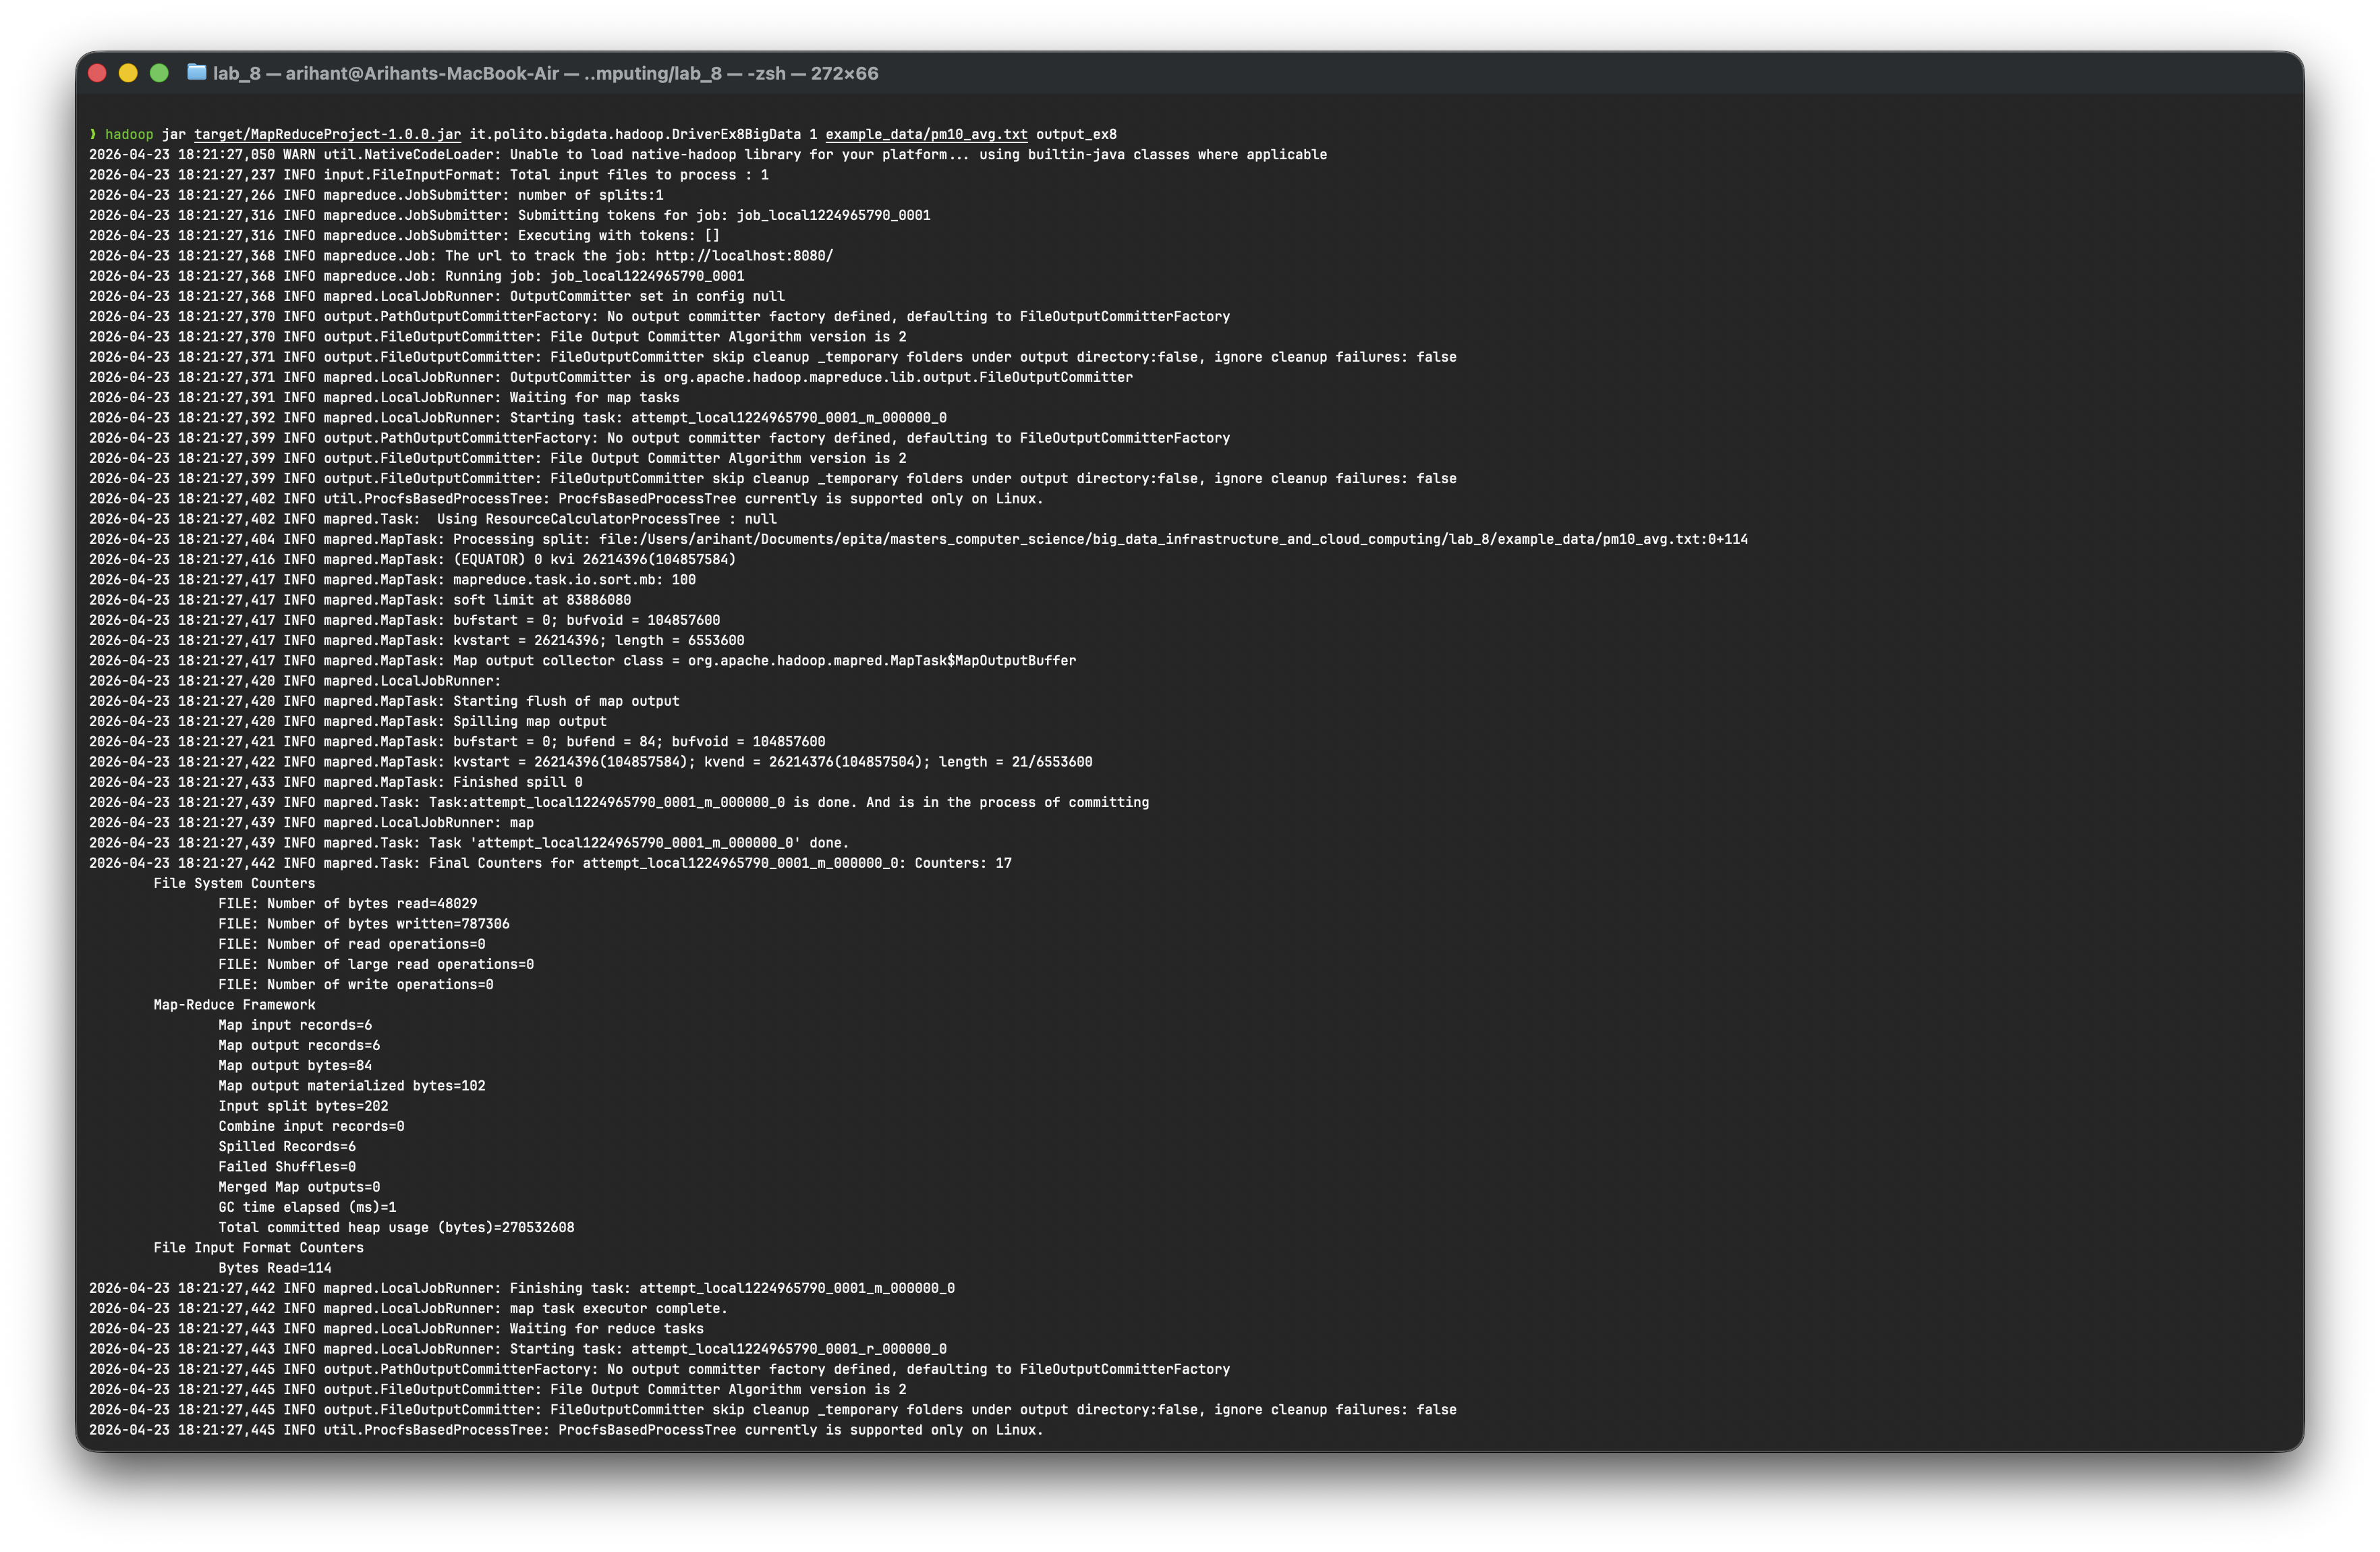
\includegraphics[width=0.75\textwidth]{screenshots/phase3/hadoop_cmd_ex8.png}
    \caption{Exercise 8 command}
\end{figure}

\begin{figure}[H]
    \centering
    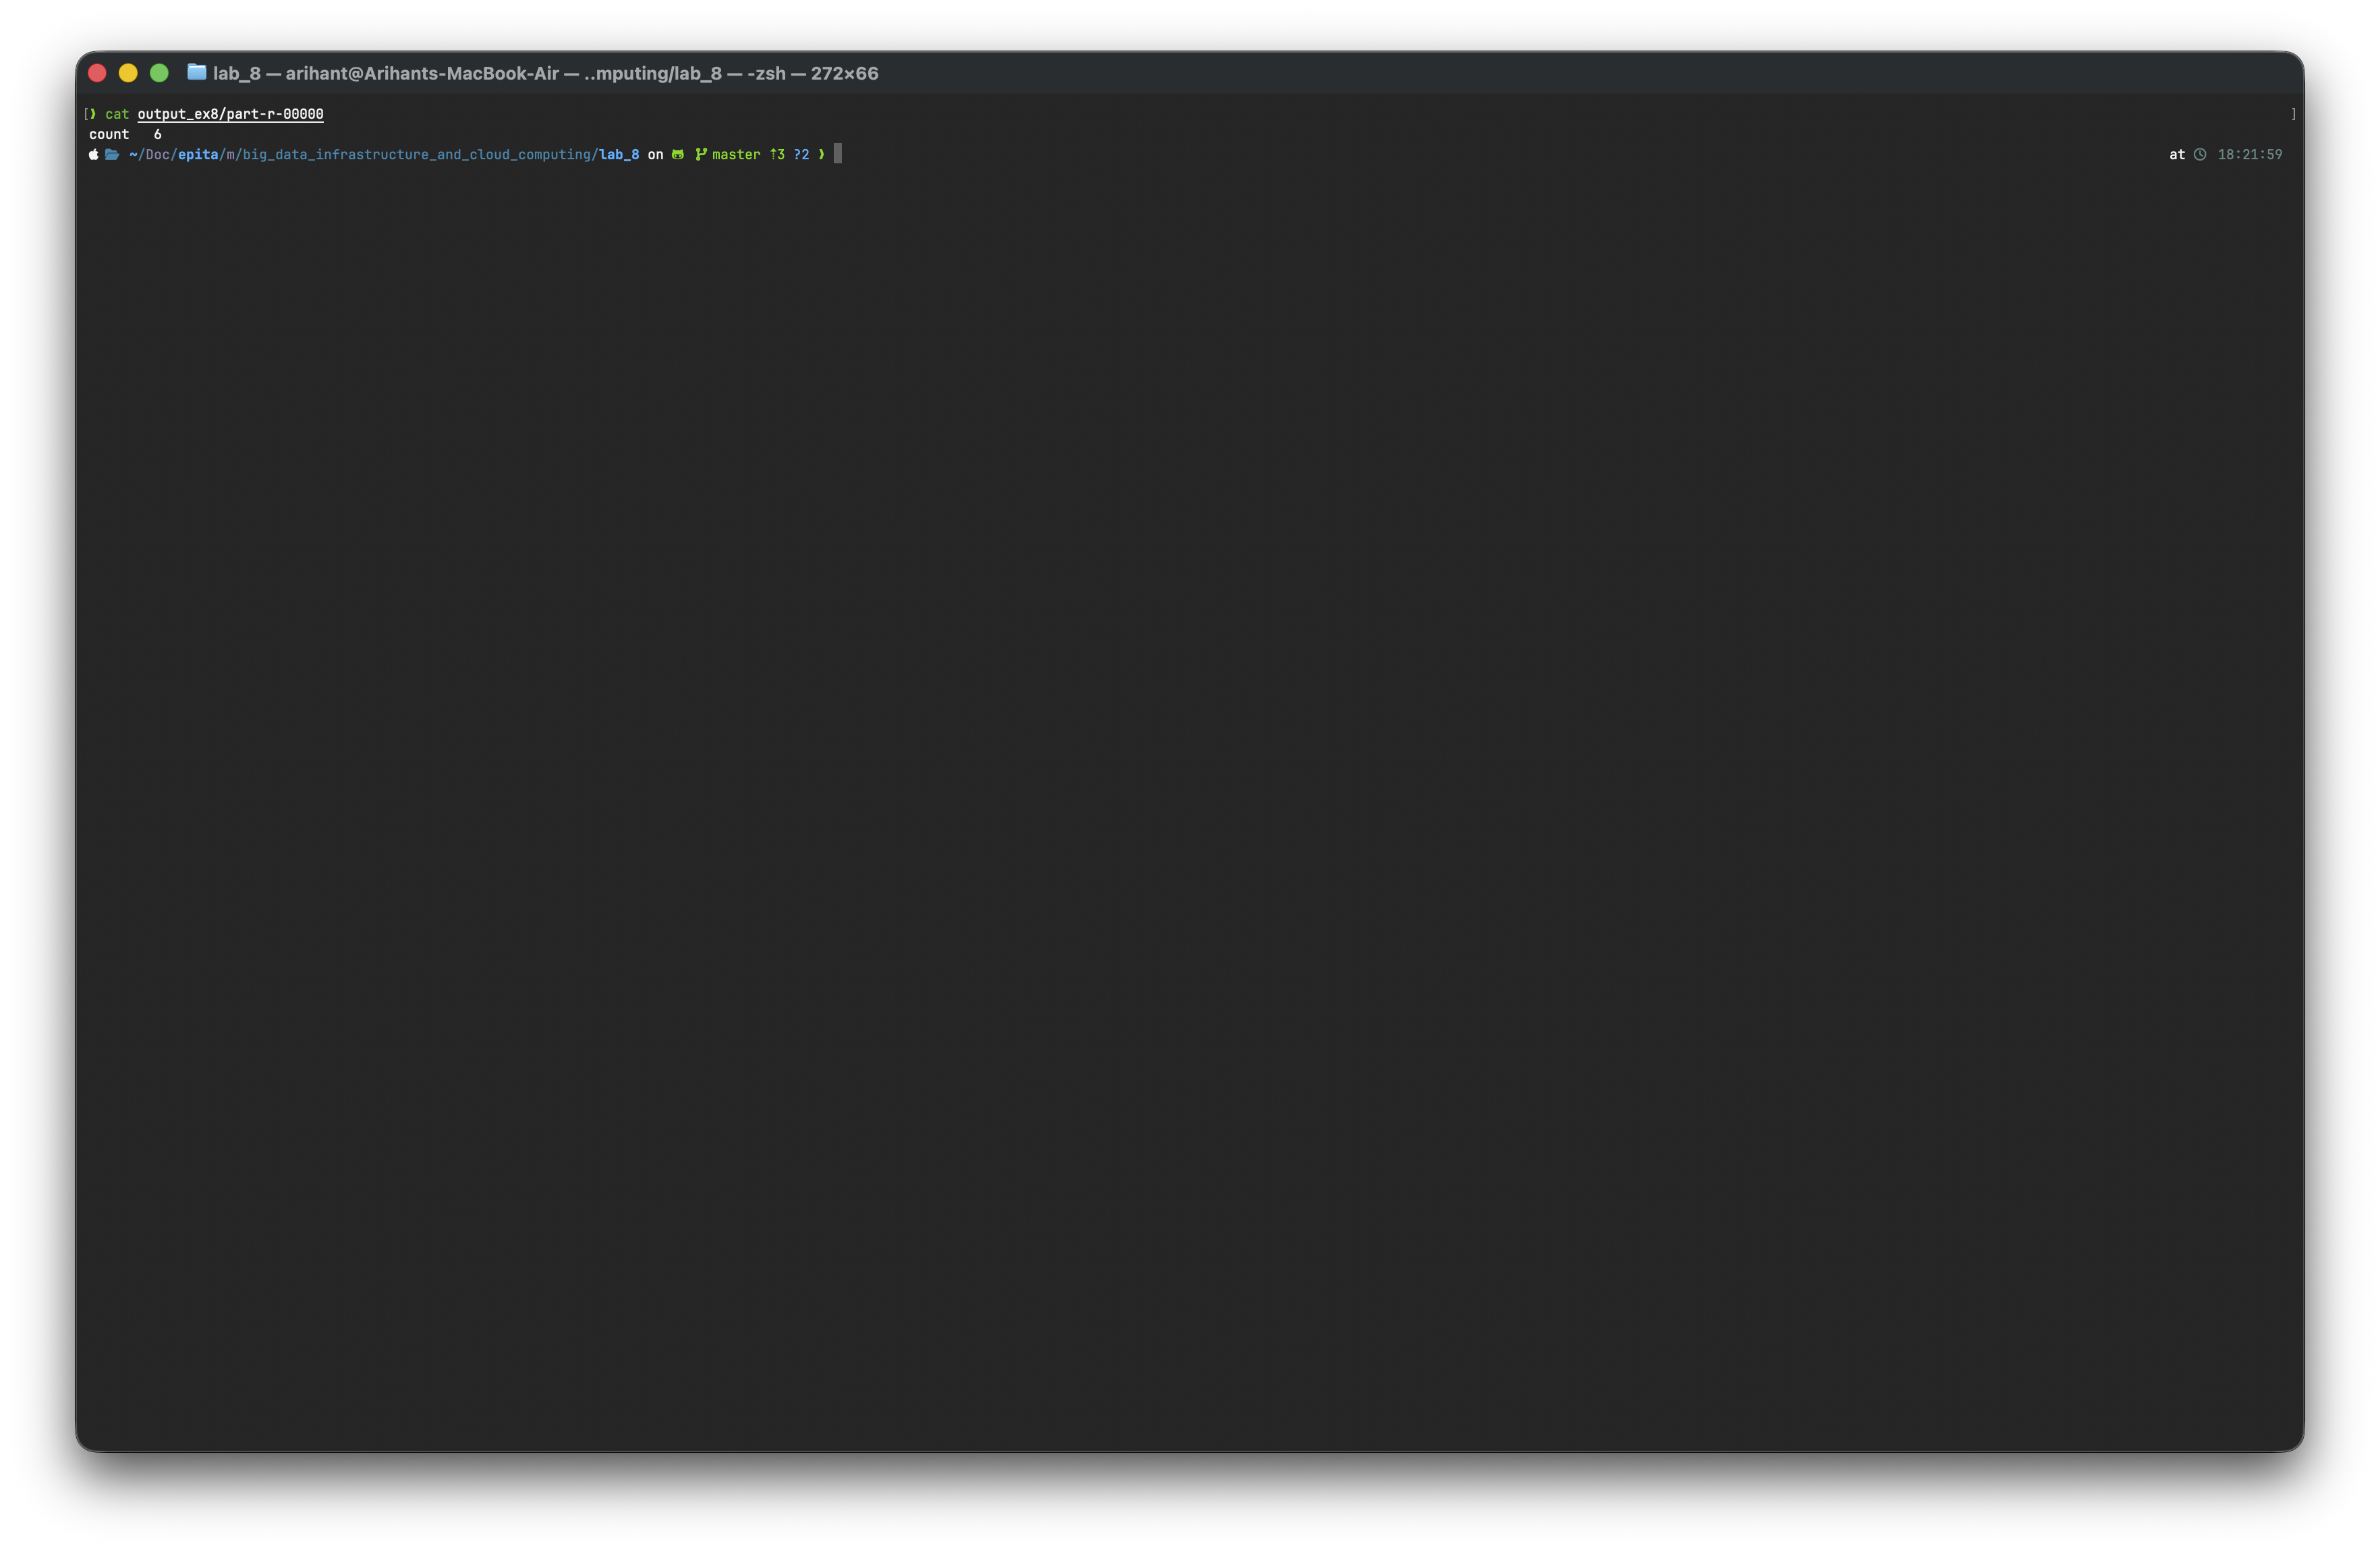
\includegraphics[width=0.75\textwidth]{screenshots/phase3/part-r-0000_ex8.png}
    \caption{Exercise 8 output}
\end{figure}

\section{Average with In-Mapper Combiner}

\subsection*{Objective}
Compute the average PM10 per sensor while reducing mapper output.

\subsection*{Implementation}
The mapper stores partial sums and counts in a local hash map. In \texttt{cleanup()}, it emits one aggregated record per sensor.

\subsection*{Result}
The output gives \texttt{s1 = 48.8} and \texttt{s2 = 39.8}.

\begin{figure}[H]
    \centering
    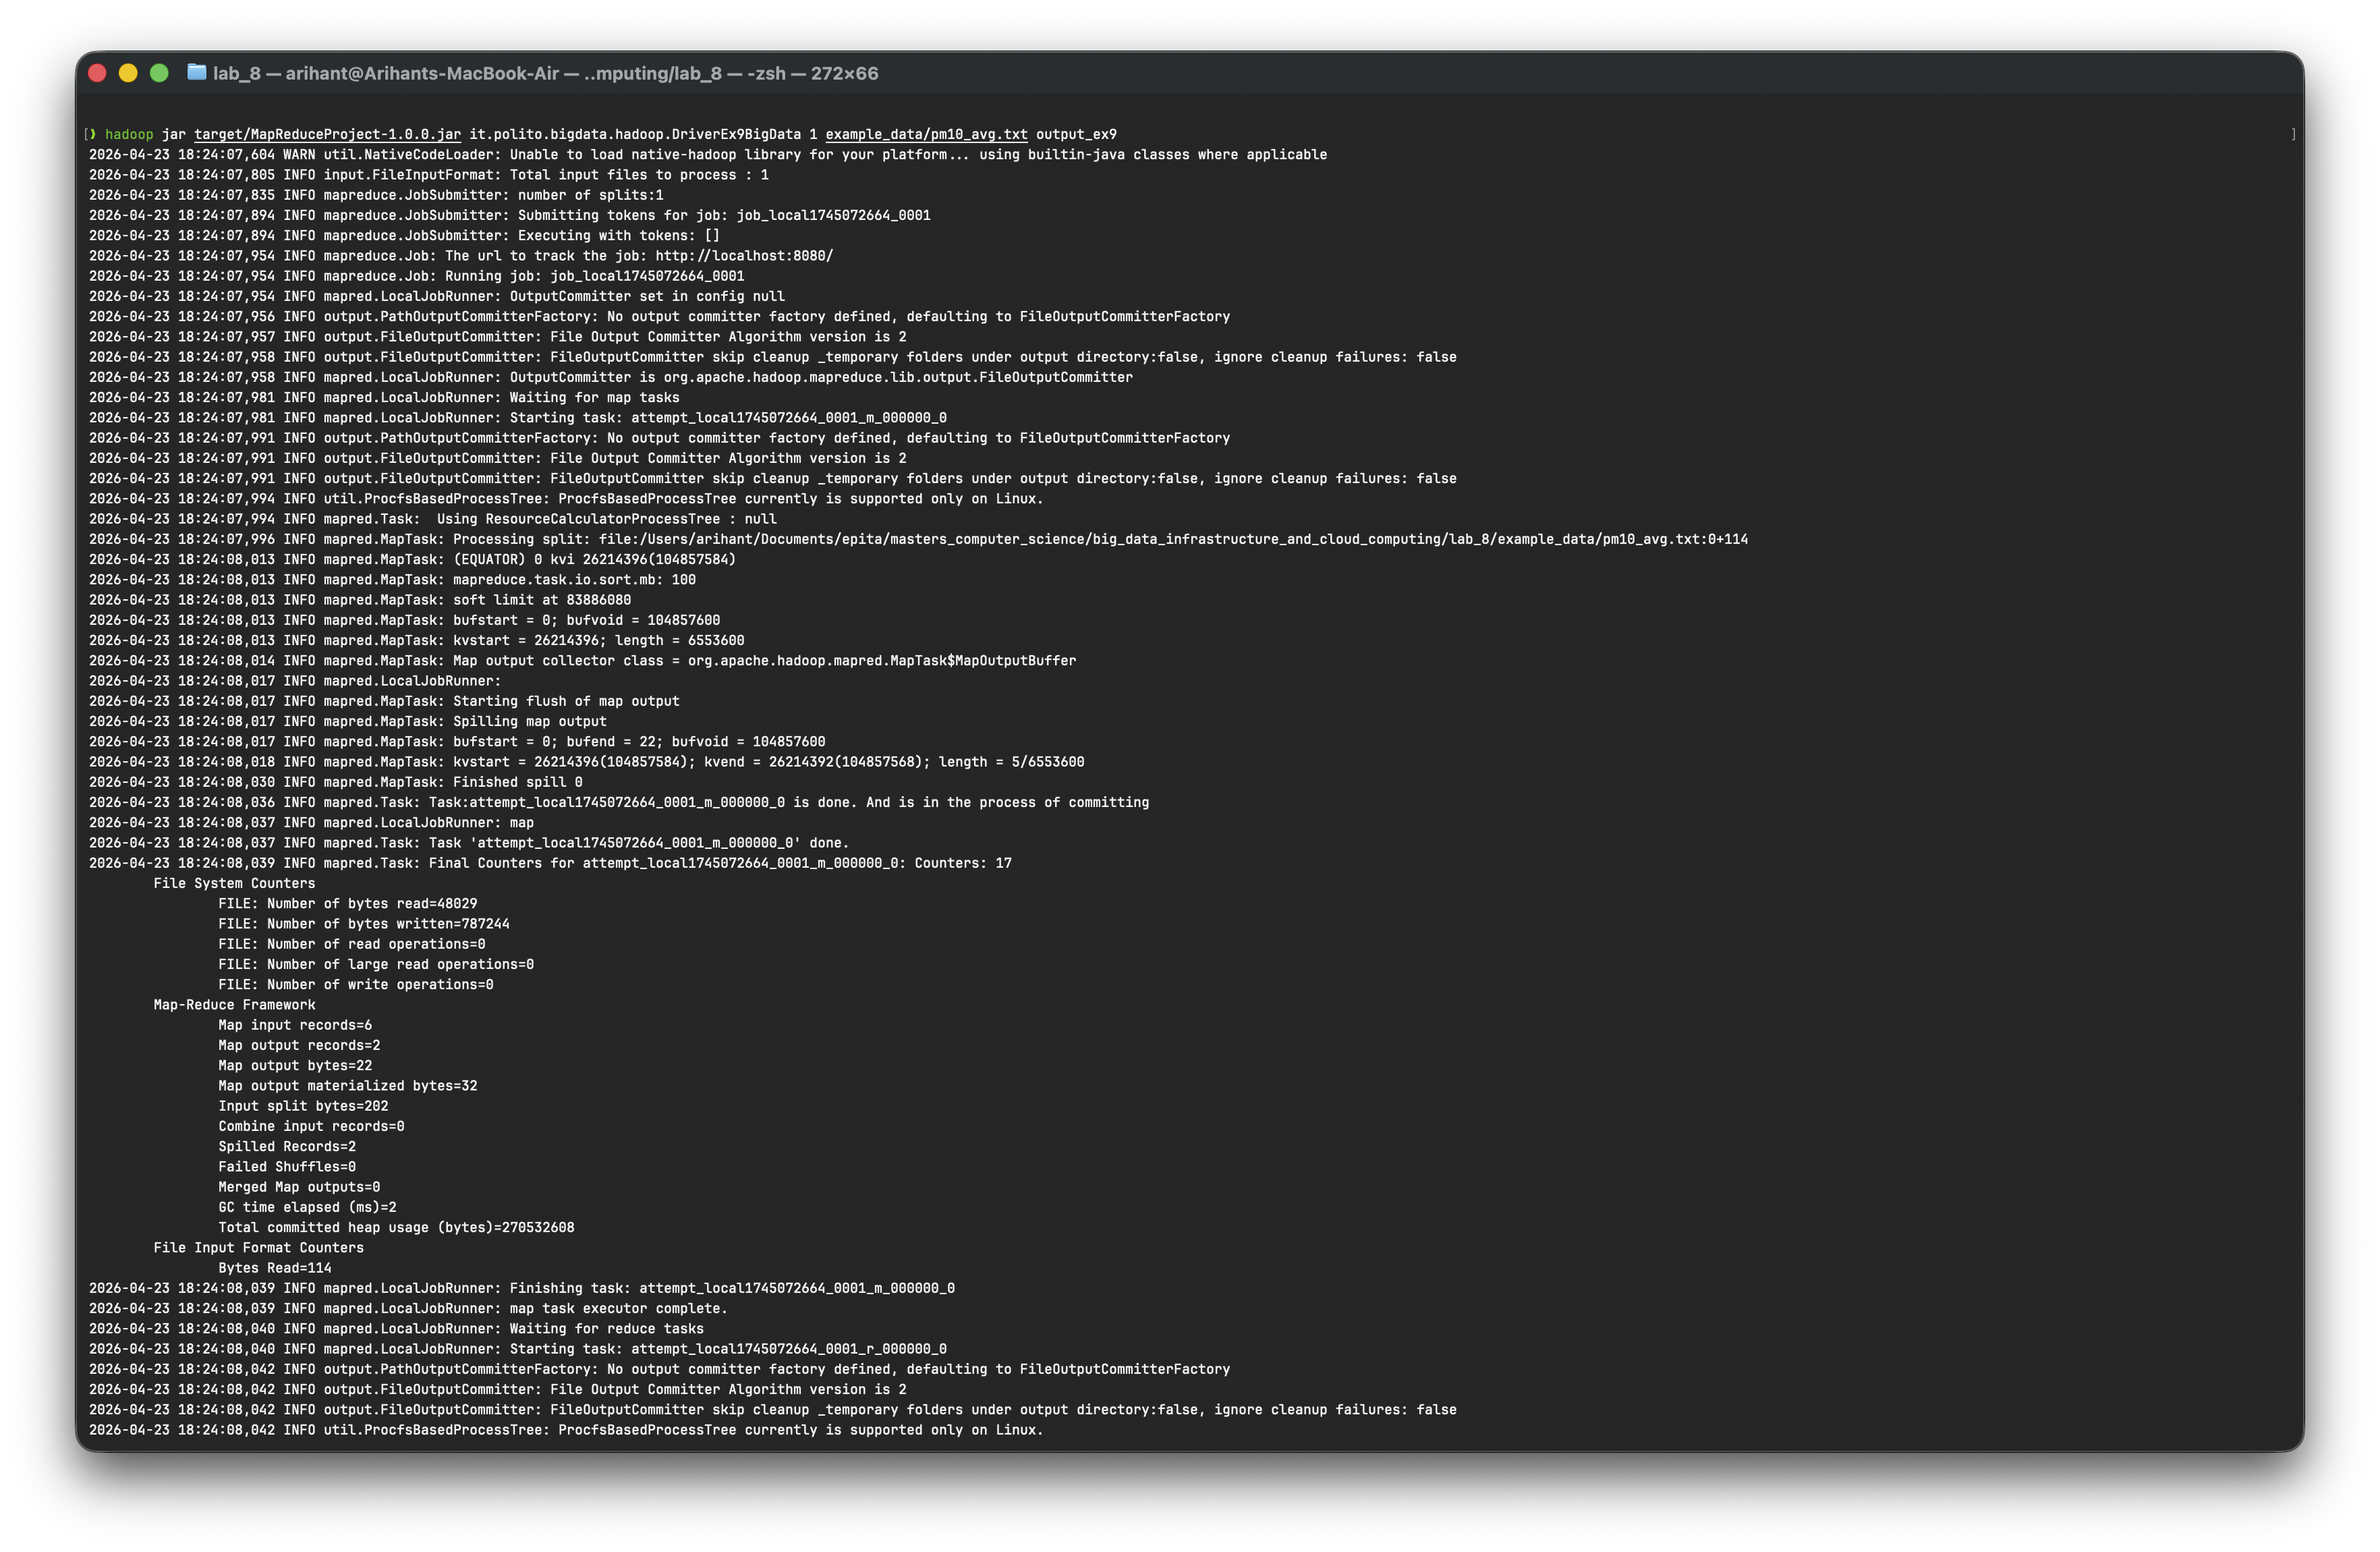
\includegraphics[width=0.75\textwidth]{screenshots/phase3/hadoop_cmd_ex9.png}
    \caption{Exercise 9 command}
\end{figure}

\begin{figure}[H]
    \centering
    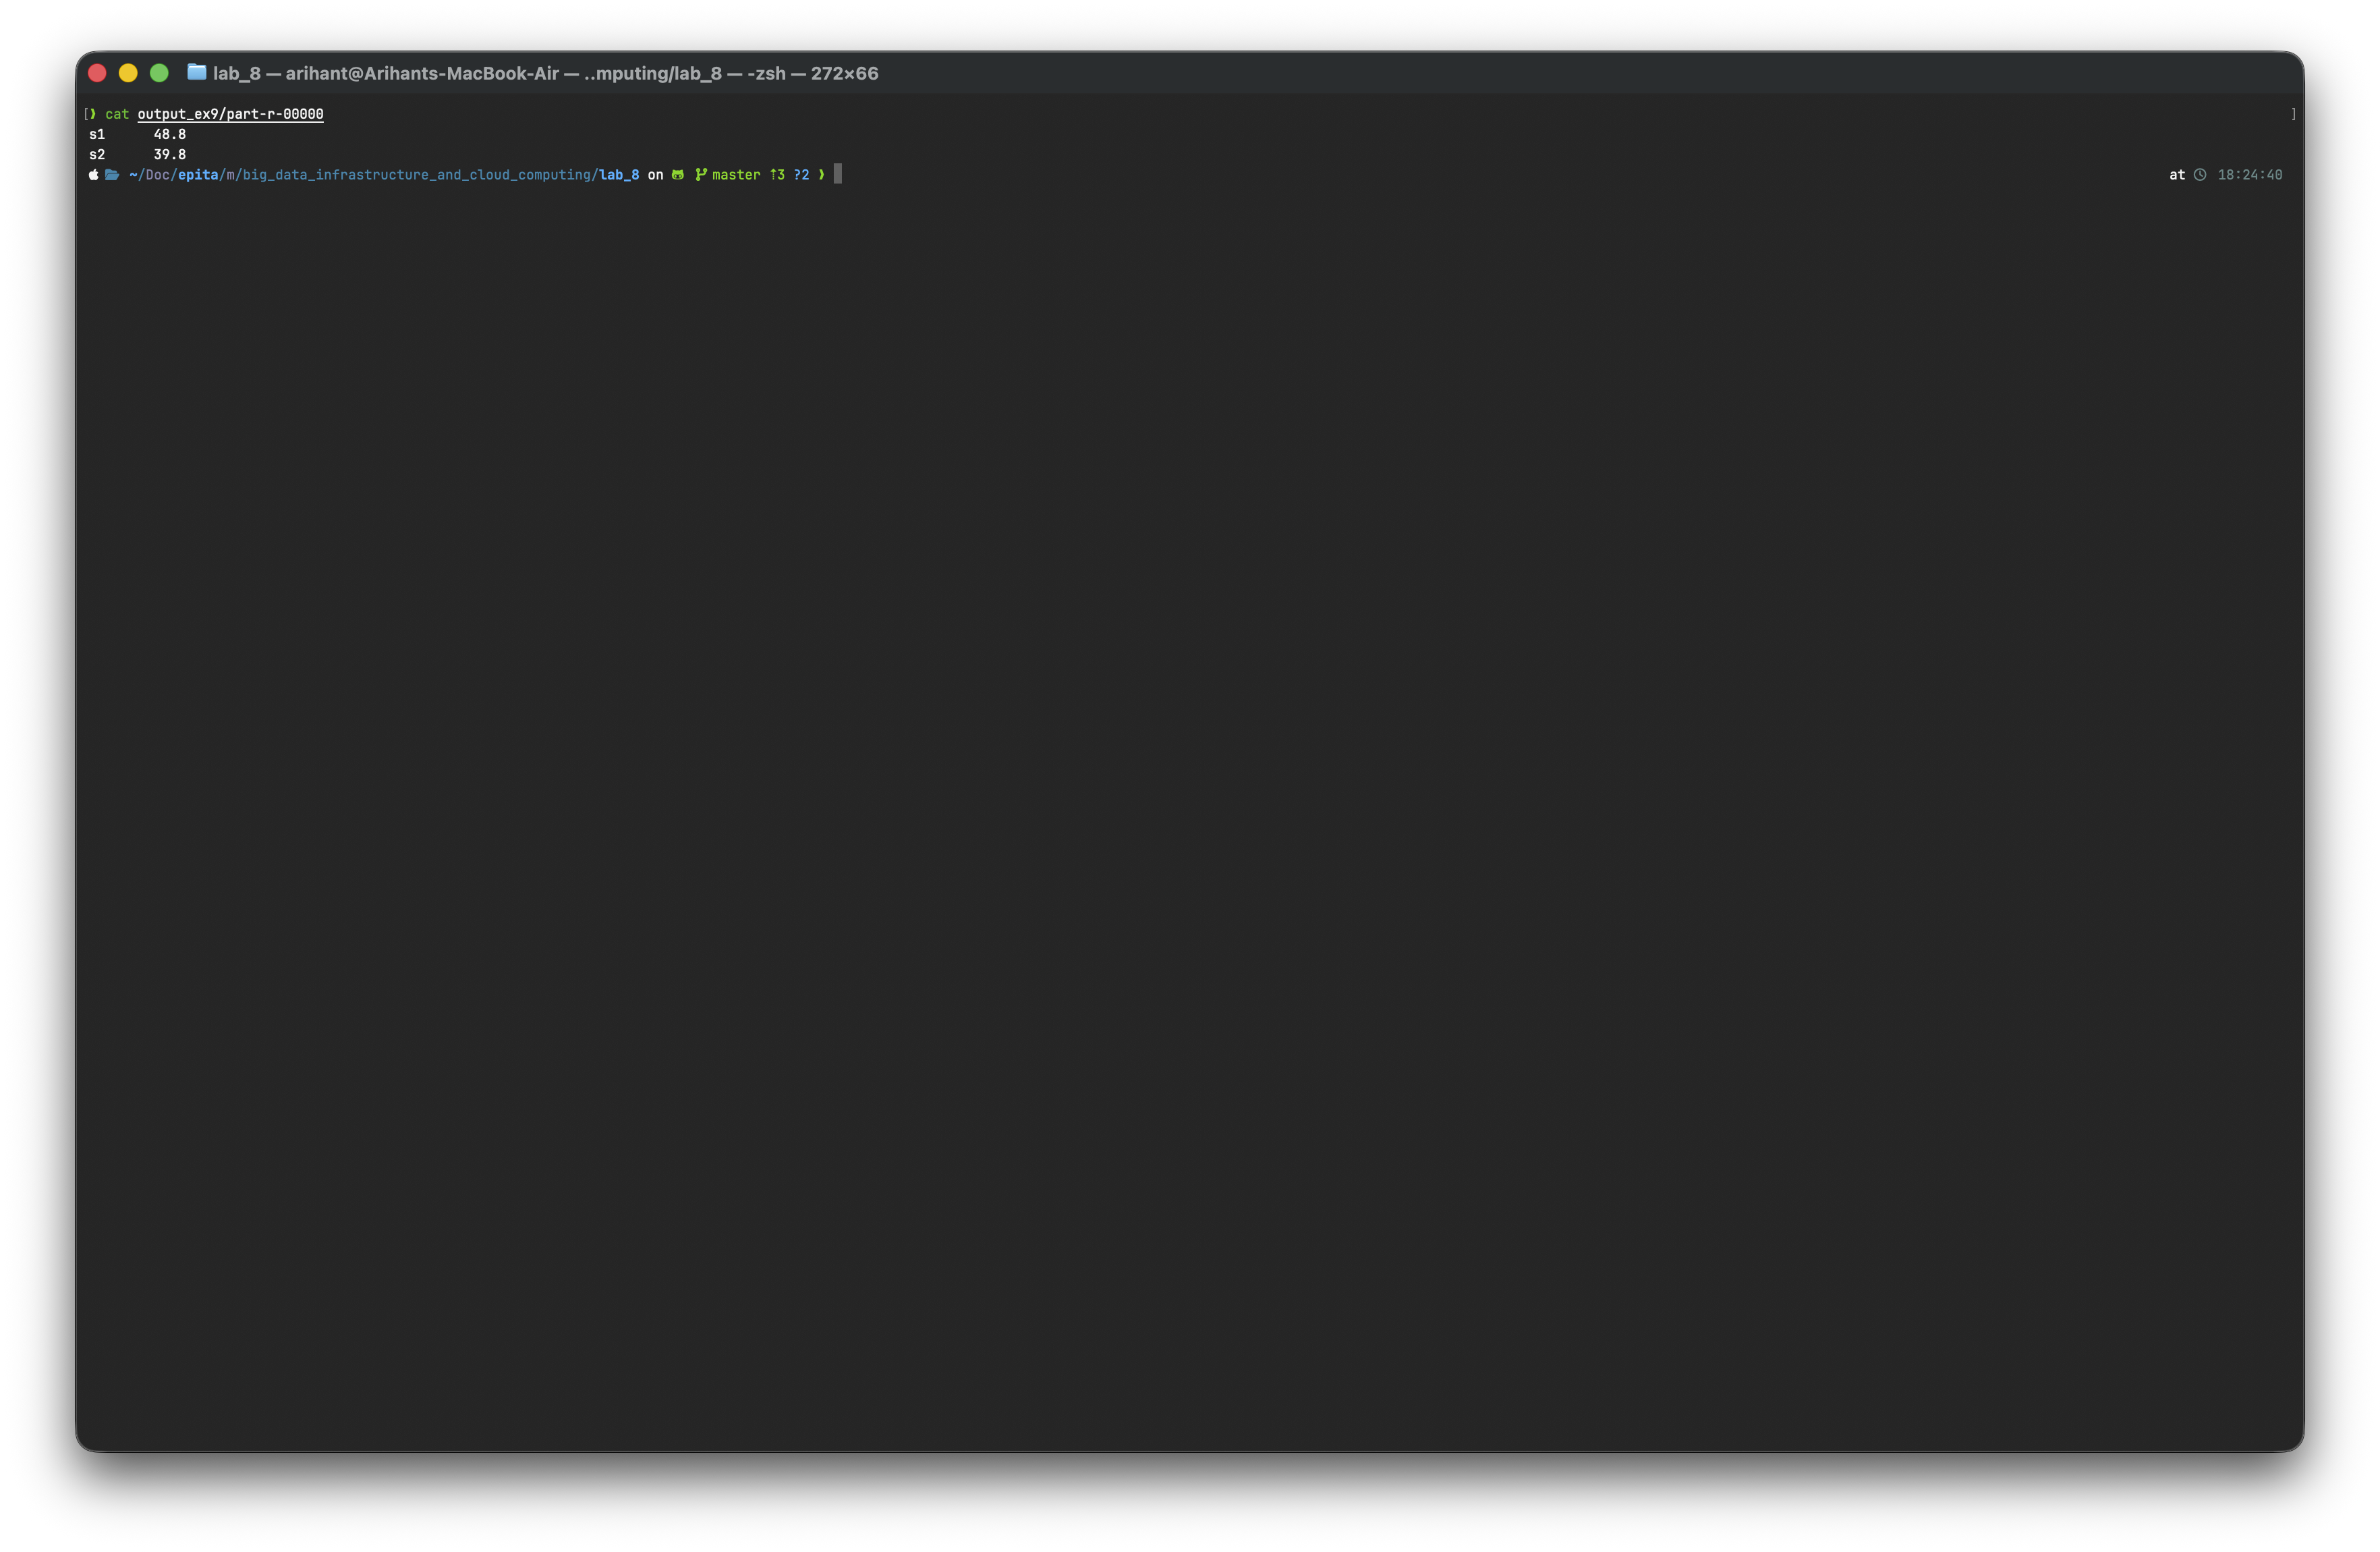
\includegraphics[width=0.75\textwidth]{screenshots/phase3/part-r-0000_ex9.png}
    \caption{Exercise 9 output}
\end{figure}

\section{Select Outliers}

\subsection*{Objective}
Filter records whose PM10 value is below a configurable threshold.

\subsection*{Implementation}
The threshold is passed through the Hadoop configuration. The mapper reads it and emits only the records that satisfy the condition.

\subsection*{Result}
With threshold \texttt{40.0}, the sample input returns 2 records.

\begin{figure}[H]
    \centering
    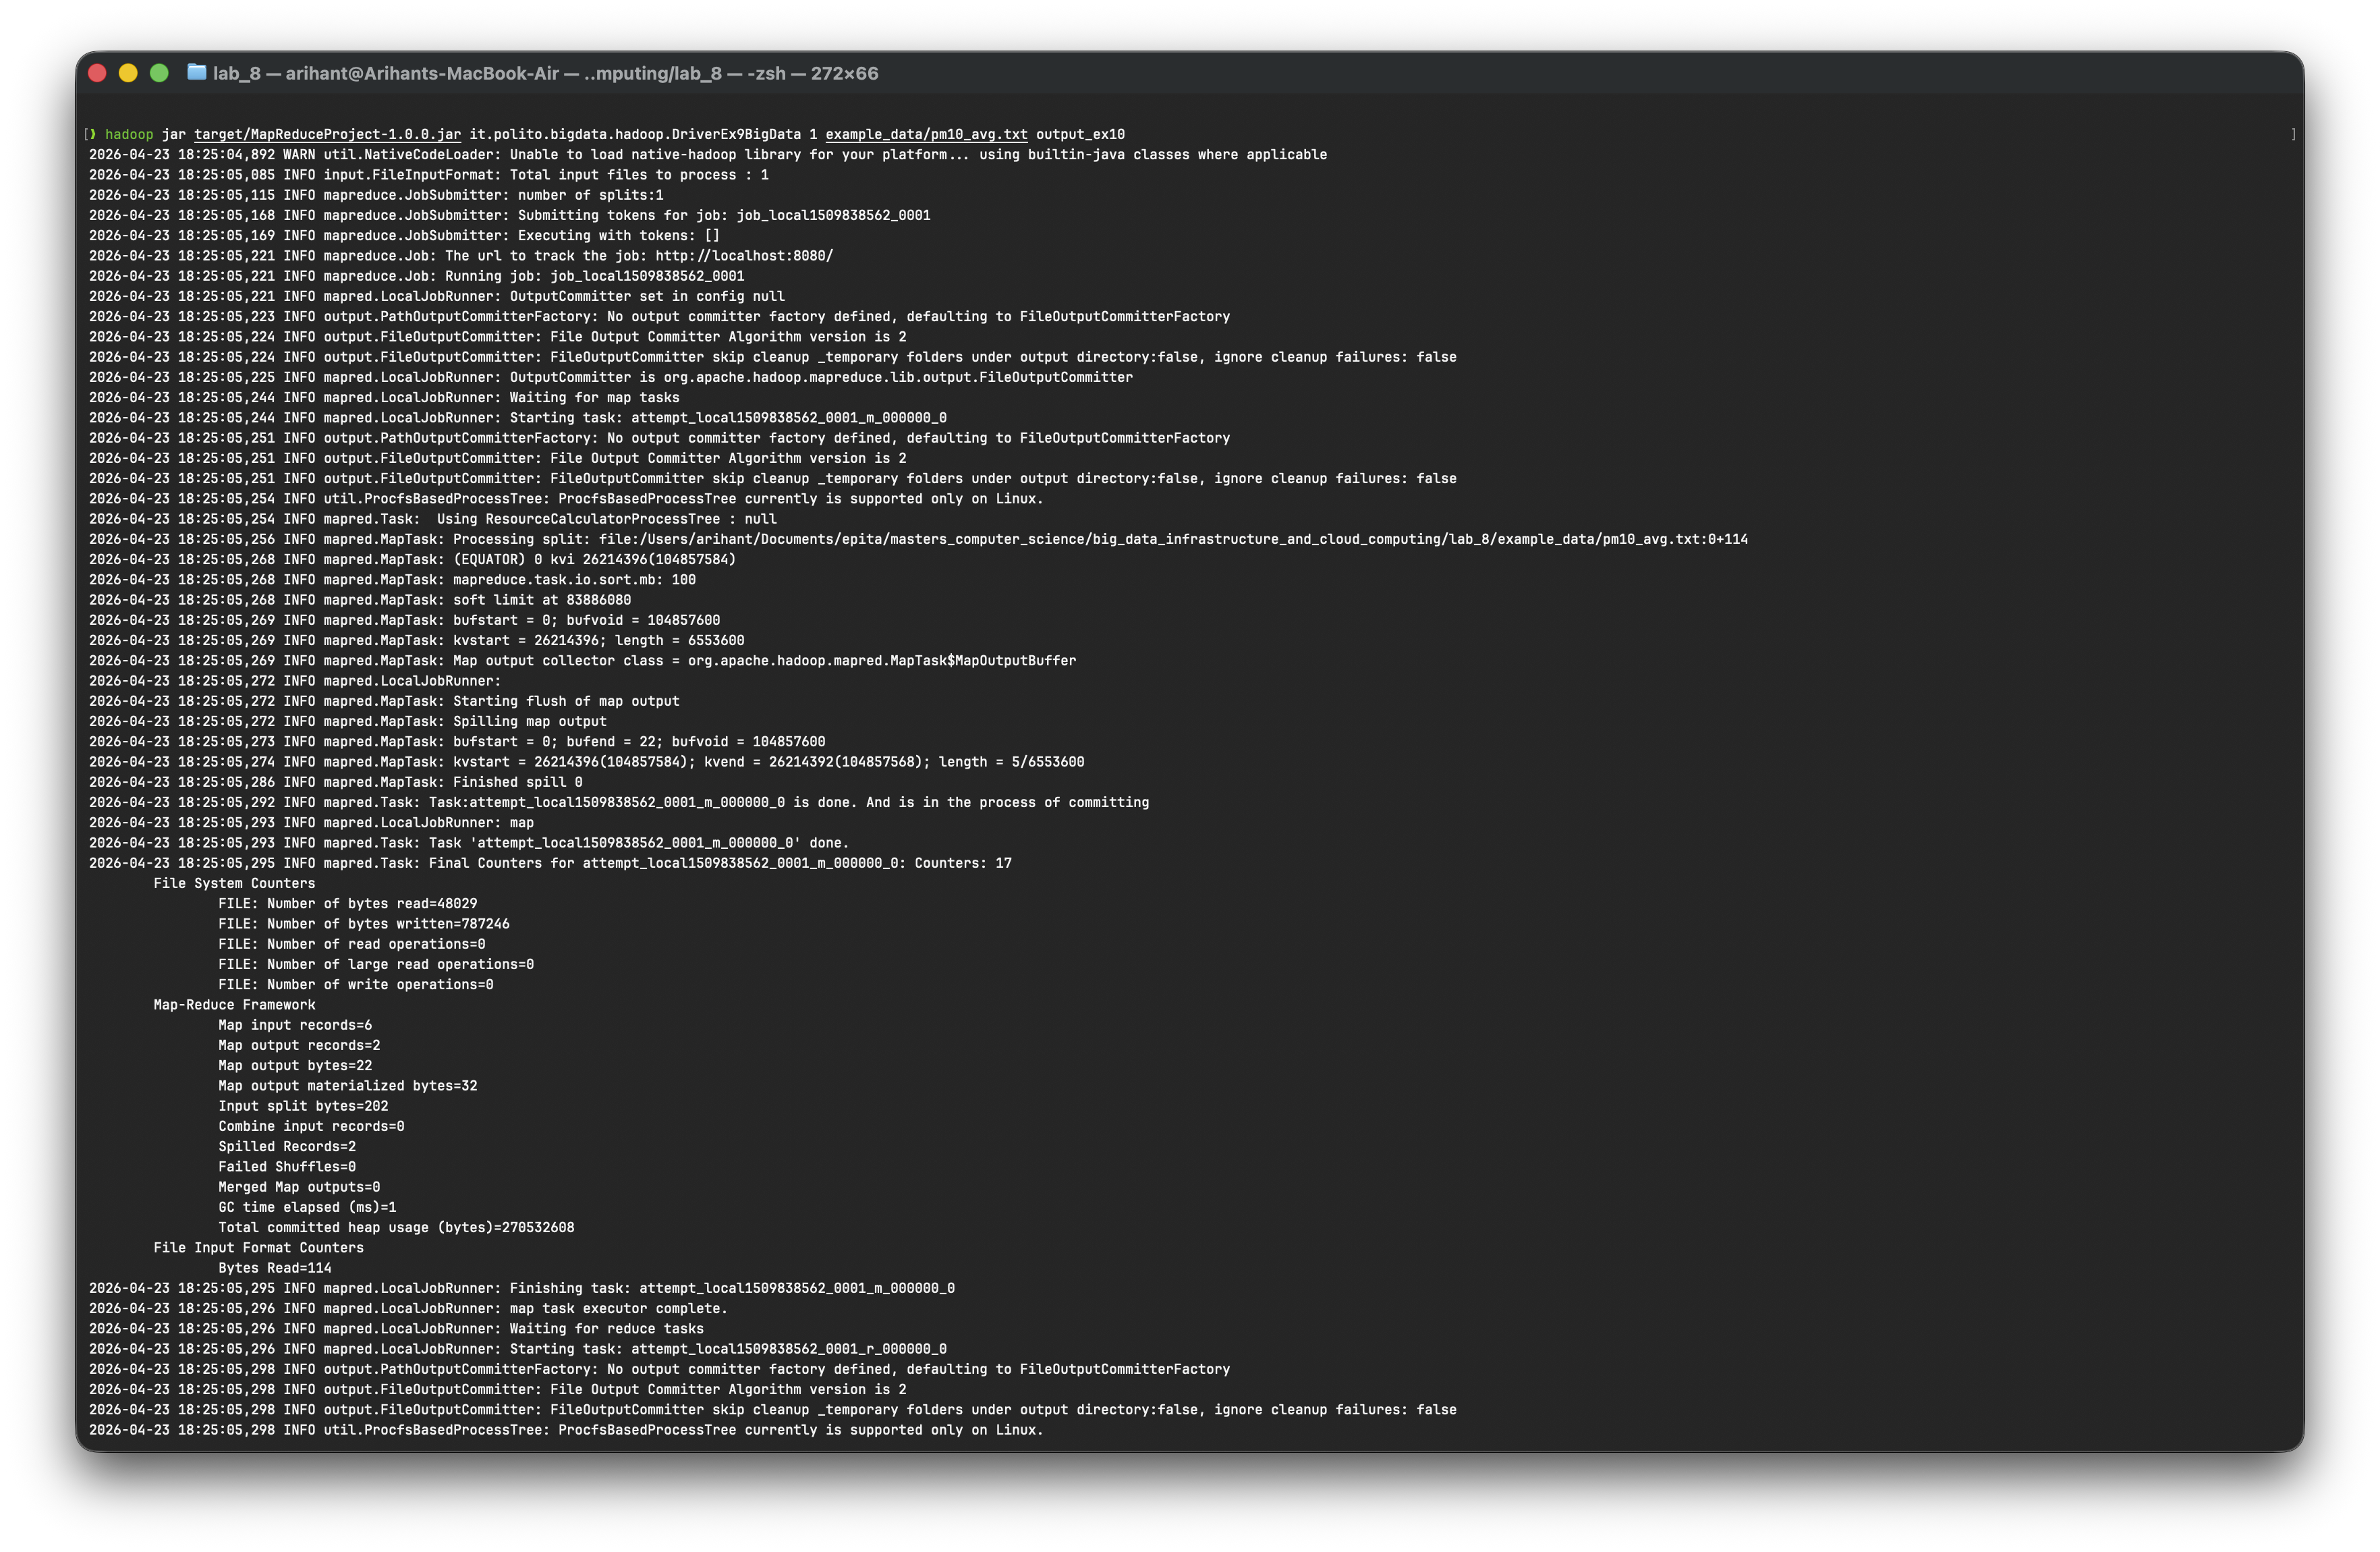
\includegraphics[width=0.75\textwidth]{screenshots/phase3/hadoop_cmd_ex10.png}
    \caption{Exercise 10 command}
\end{figure}

\begin{figure}[H]
    \centering
    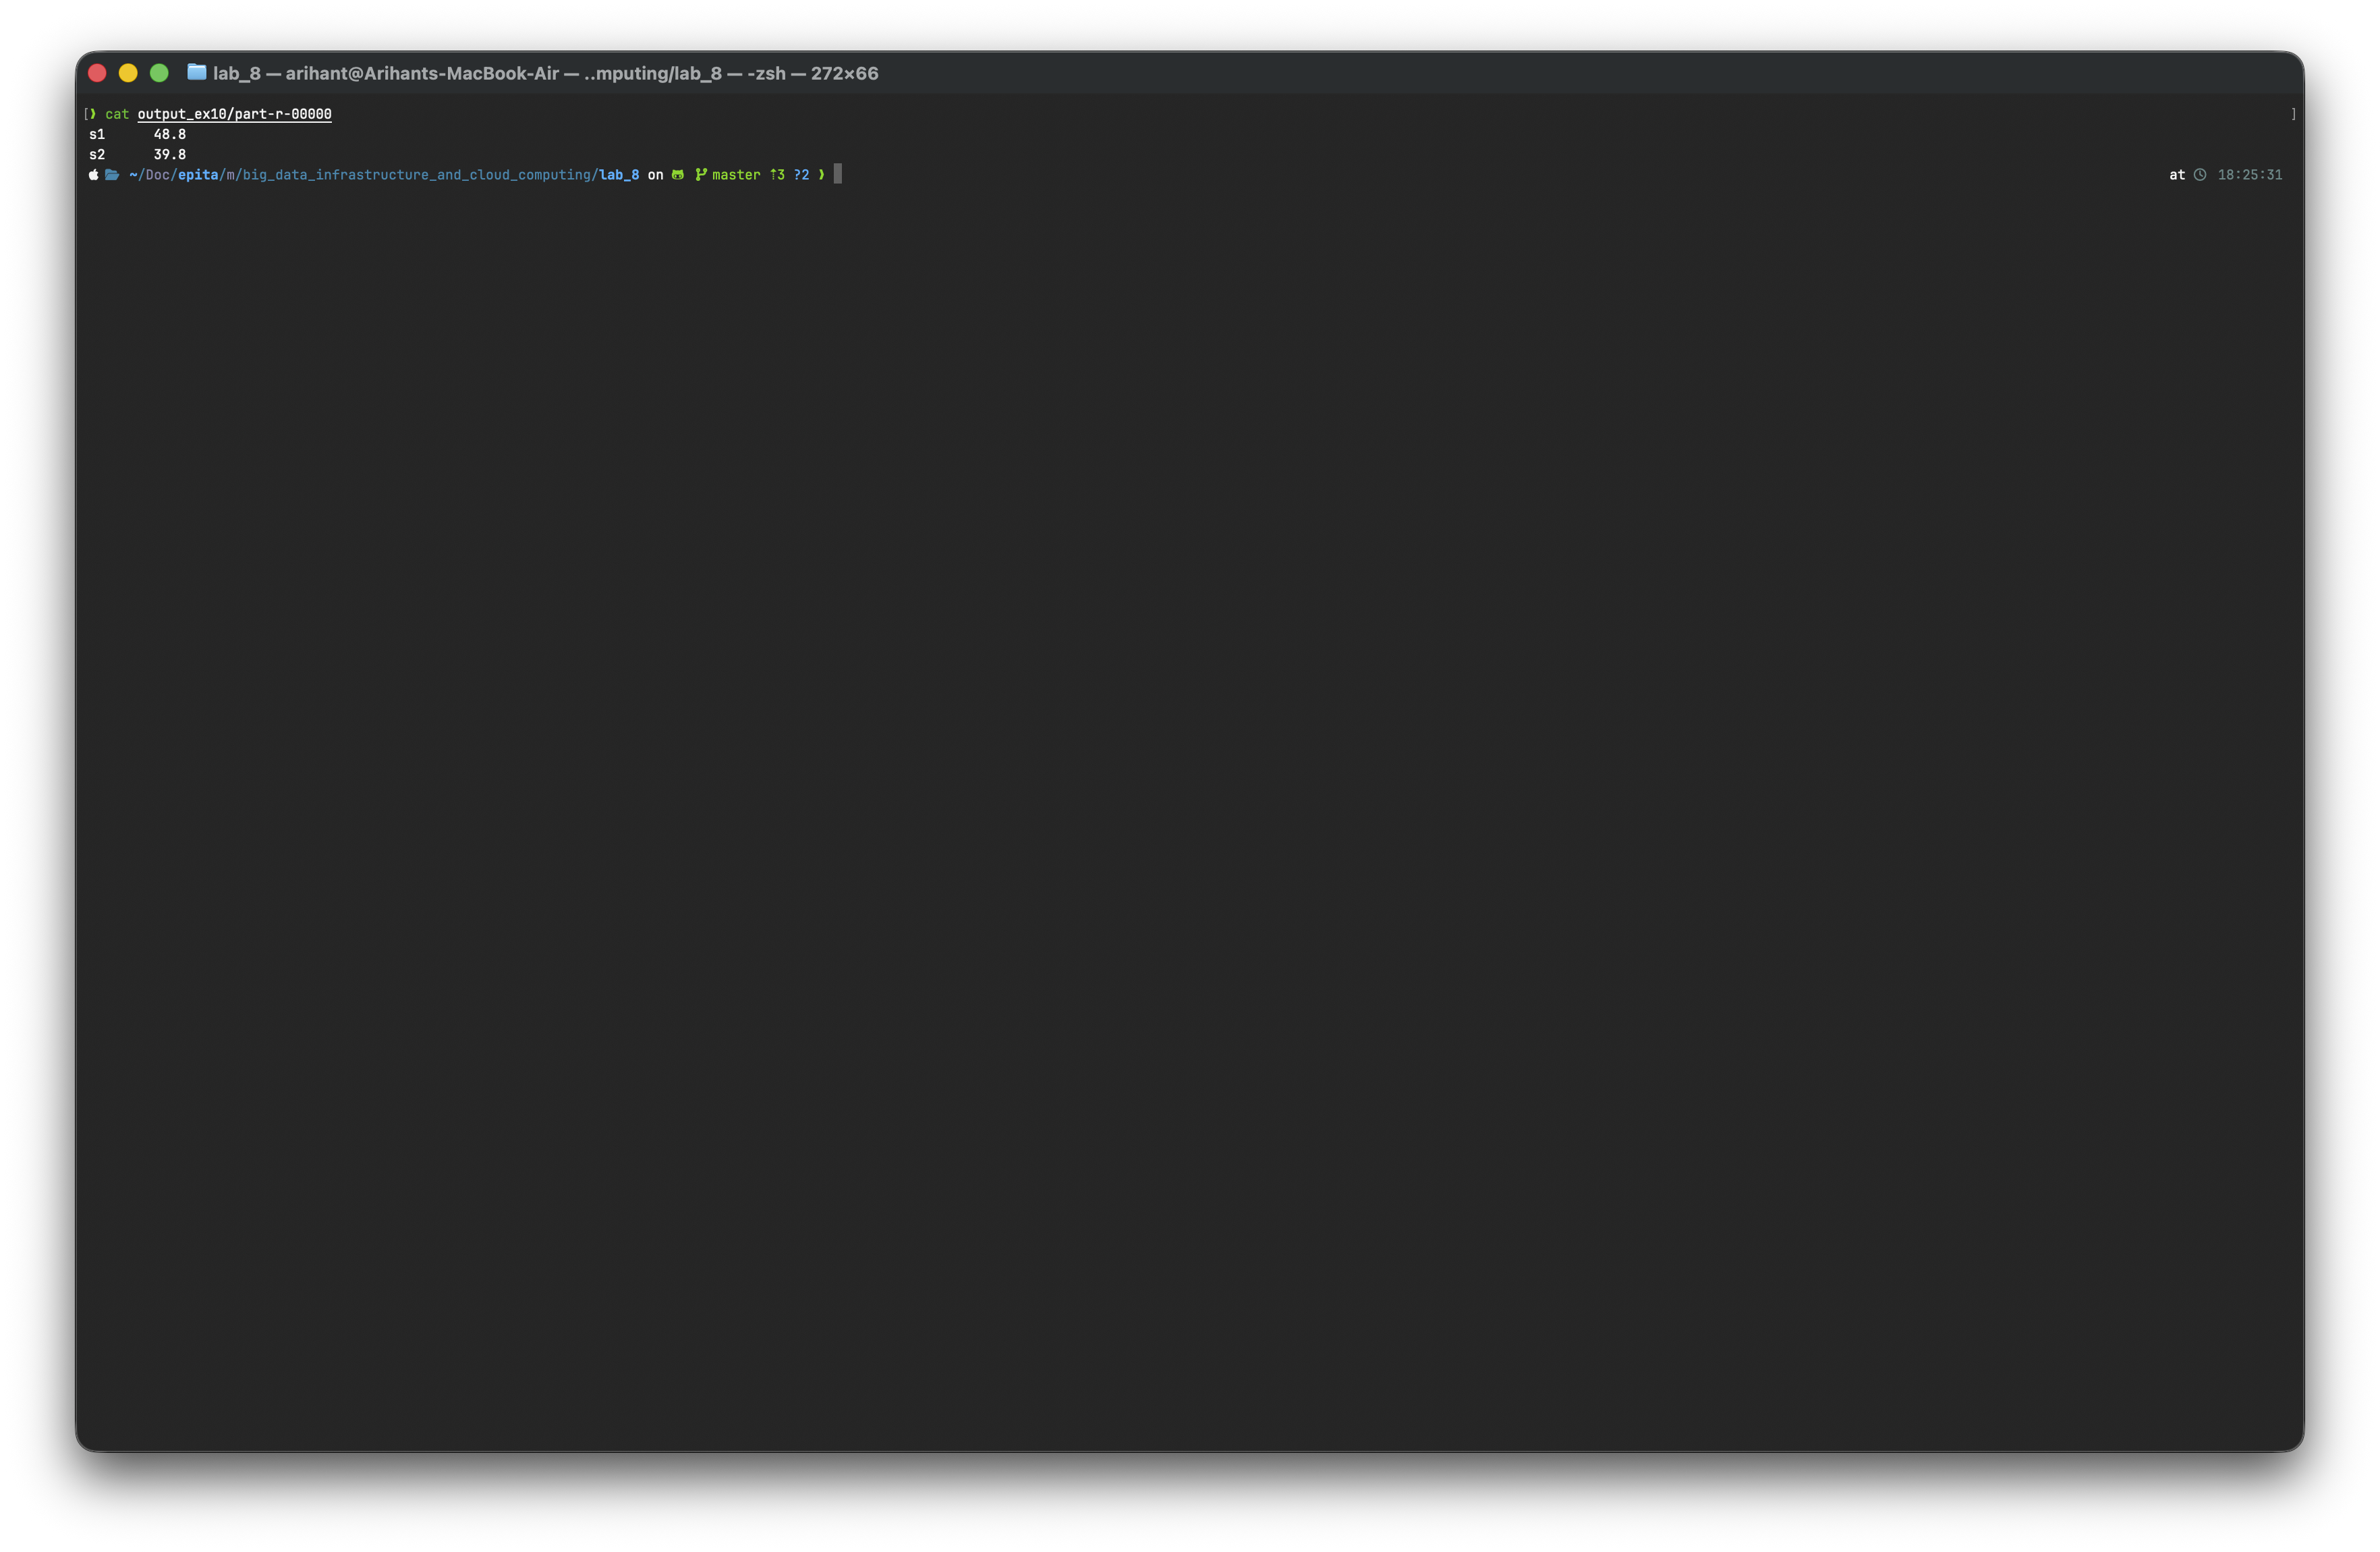
\includegraphics[width=0.75\textwidth]{screenshots/phase3/part-r-0000_ex10.png}
    \caption{Exercise 10 output}
\end{figure}

\section{Top 1 Most Profitable Date}

\subsection*{Objective}
Find the date with the highest total income.

\subsection*{Implementation}
The mapper emits the date and income value. The reducer sums the income for each date and keeps the largest total.

\subsection*{Result}
The most profitable date in the sample data is \texttt{2024-01-04} with income \texttt{3100}.

\begin{figure}[H]
    \centering
    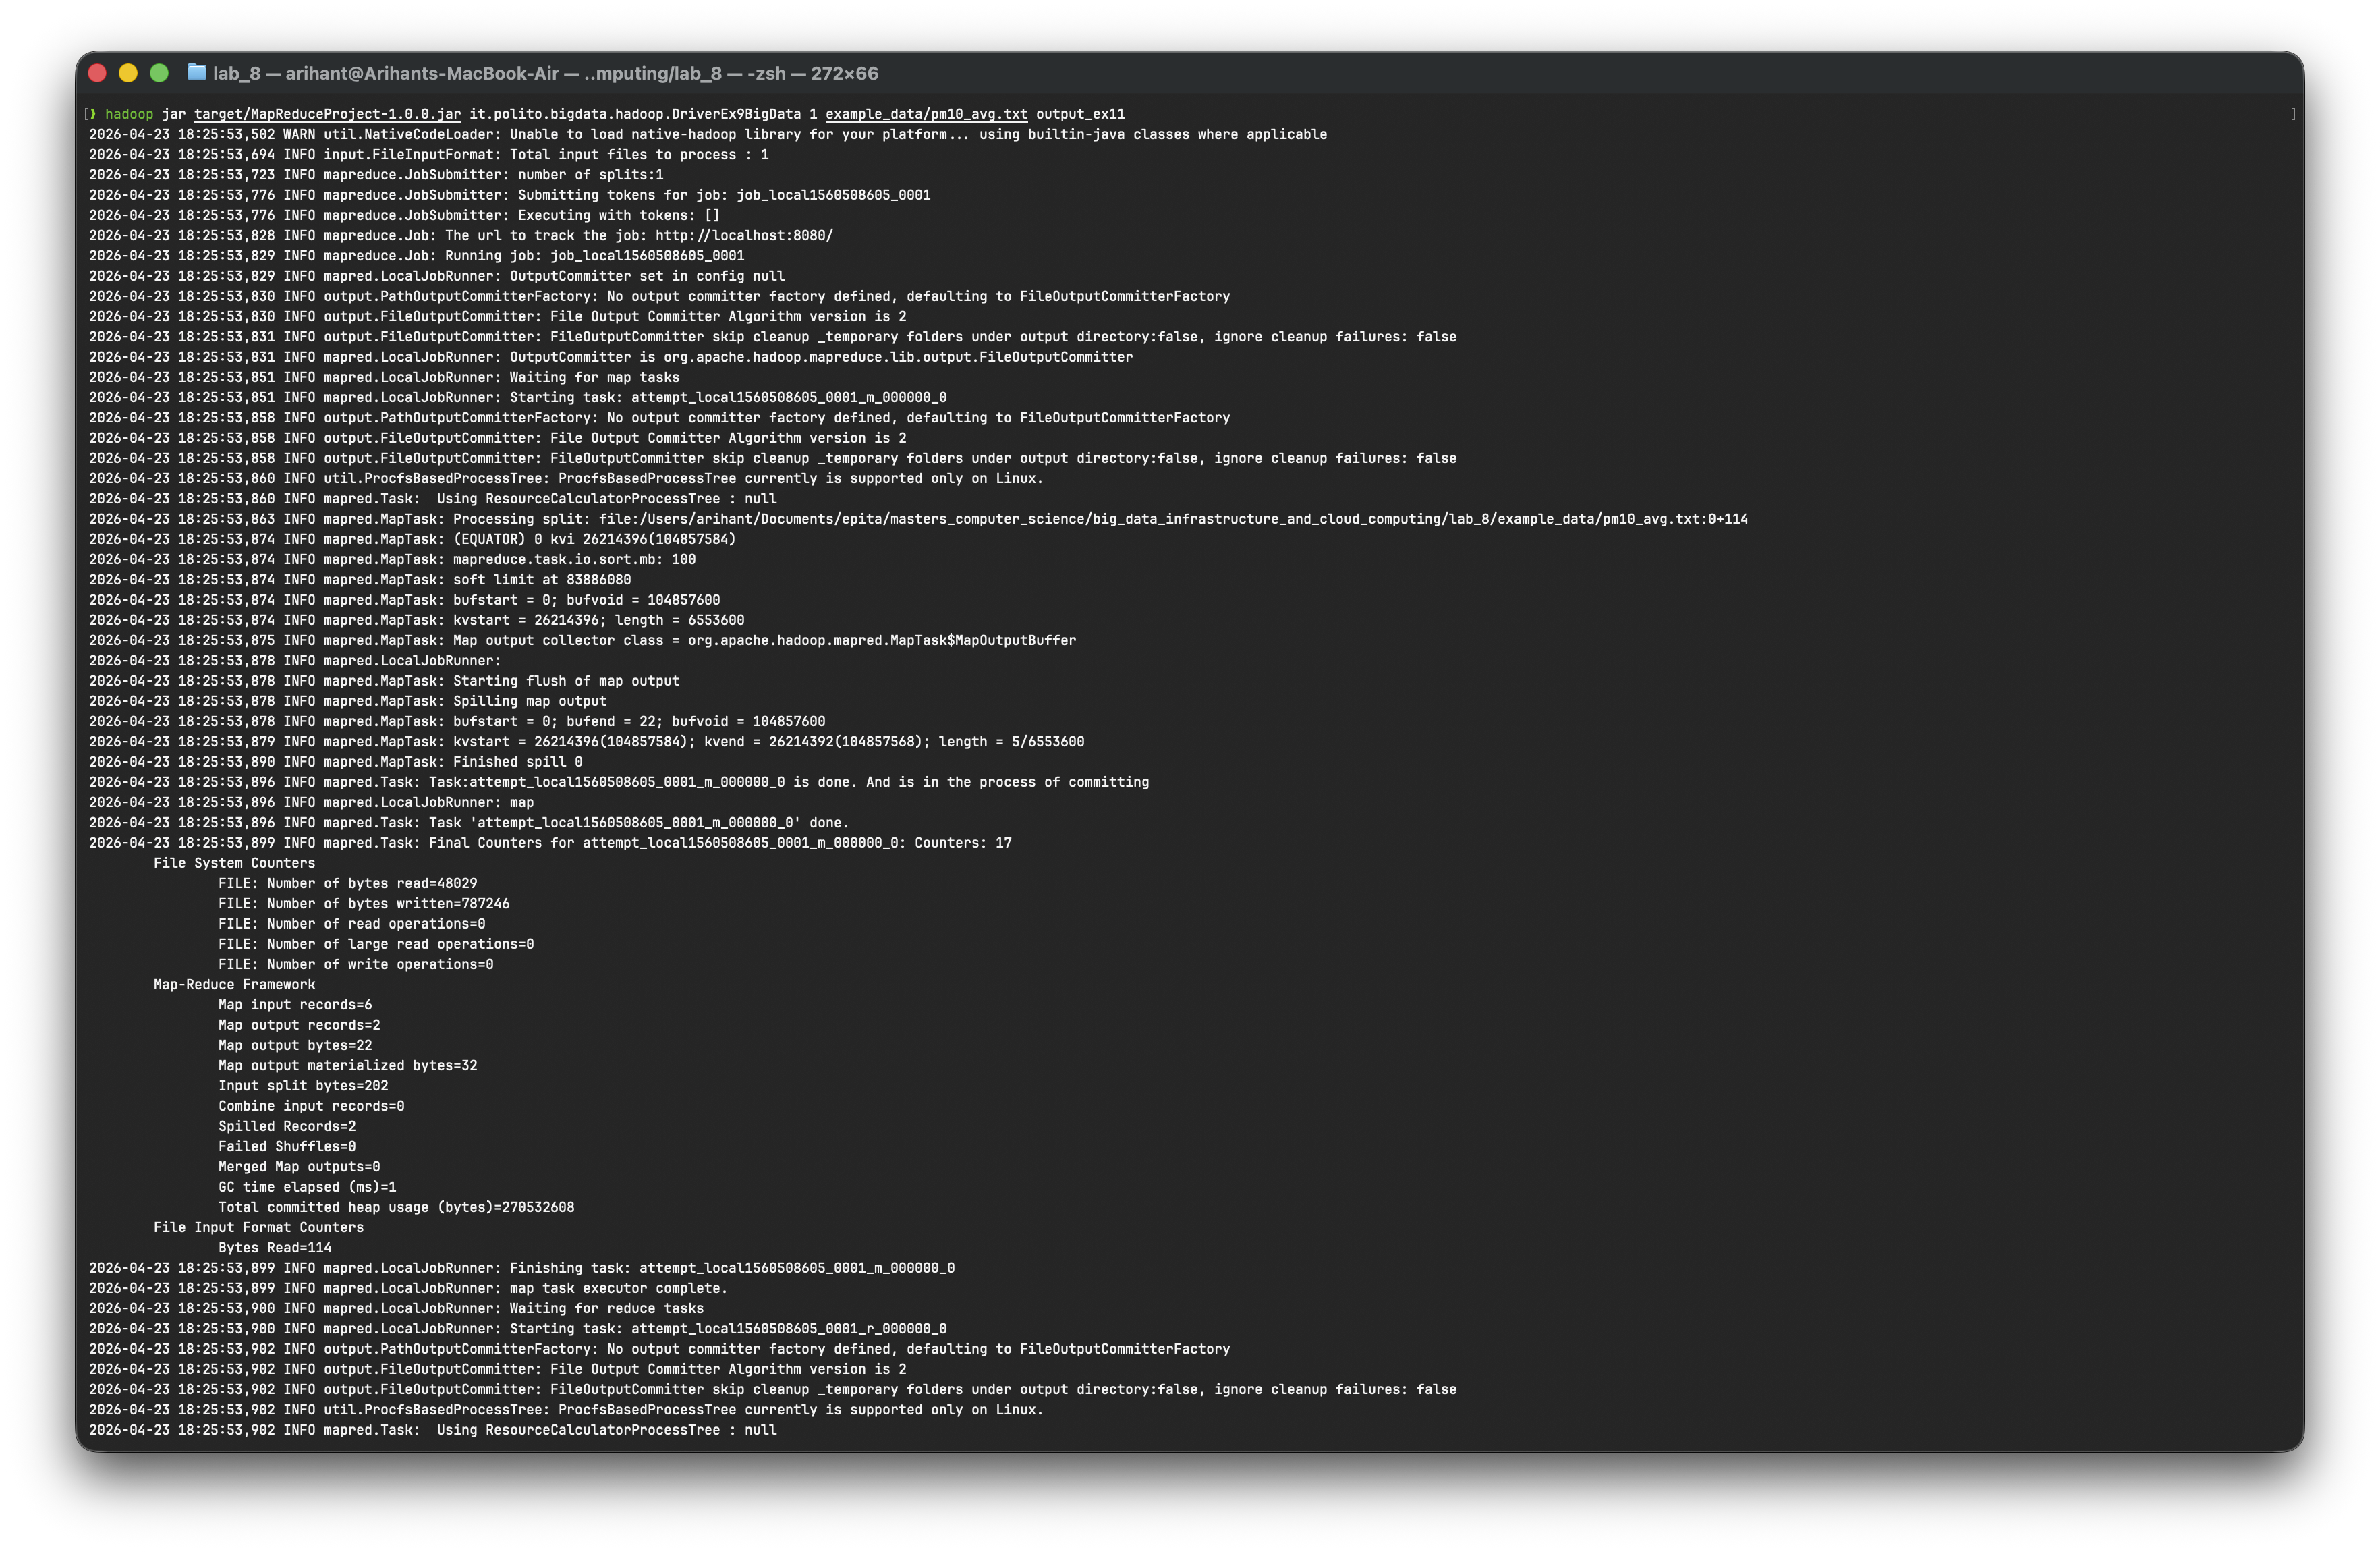
\includegraphics[width=0.75\textwidth]{screenshots/phase3/hadoop_cmd_ex11.png}
    \caption{Exercise 11 command}
\end{figure}

\begin{figure}[H]
    \centering
    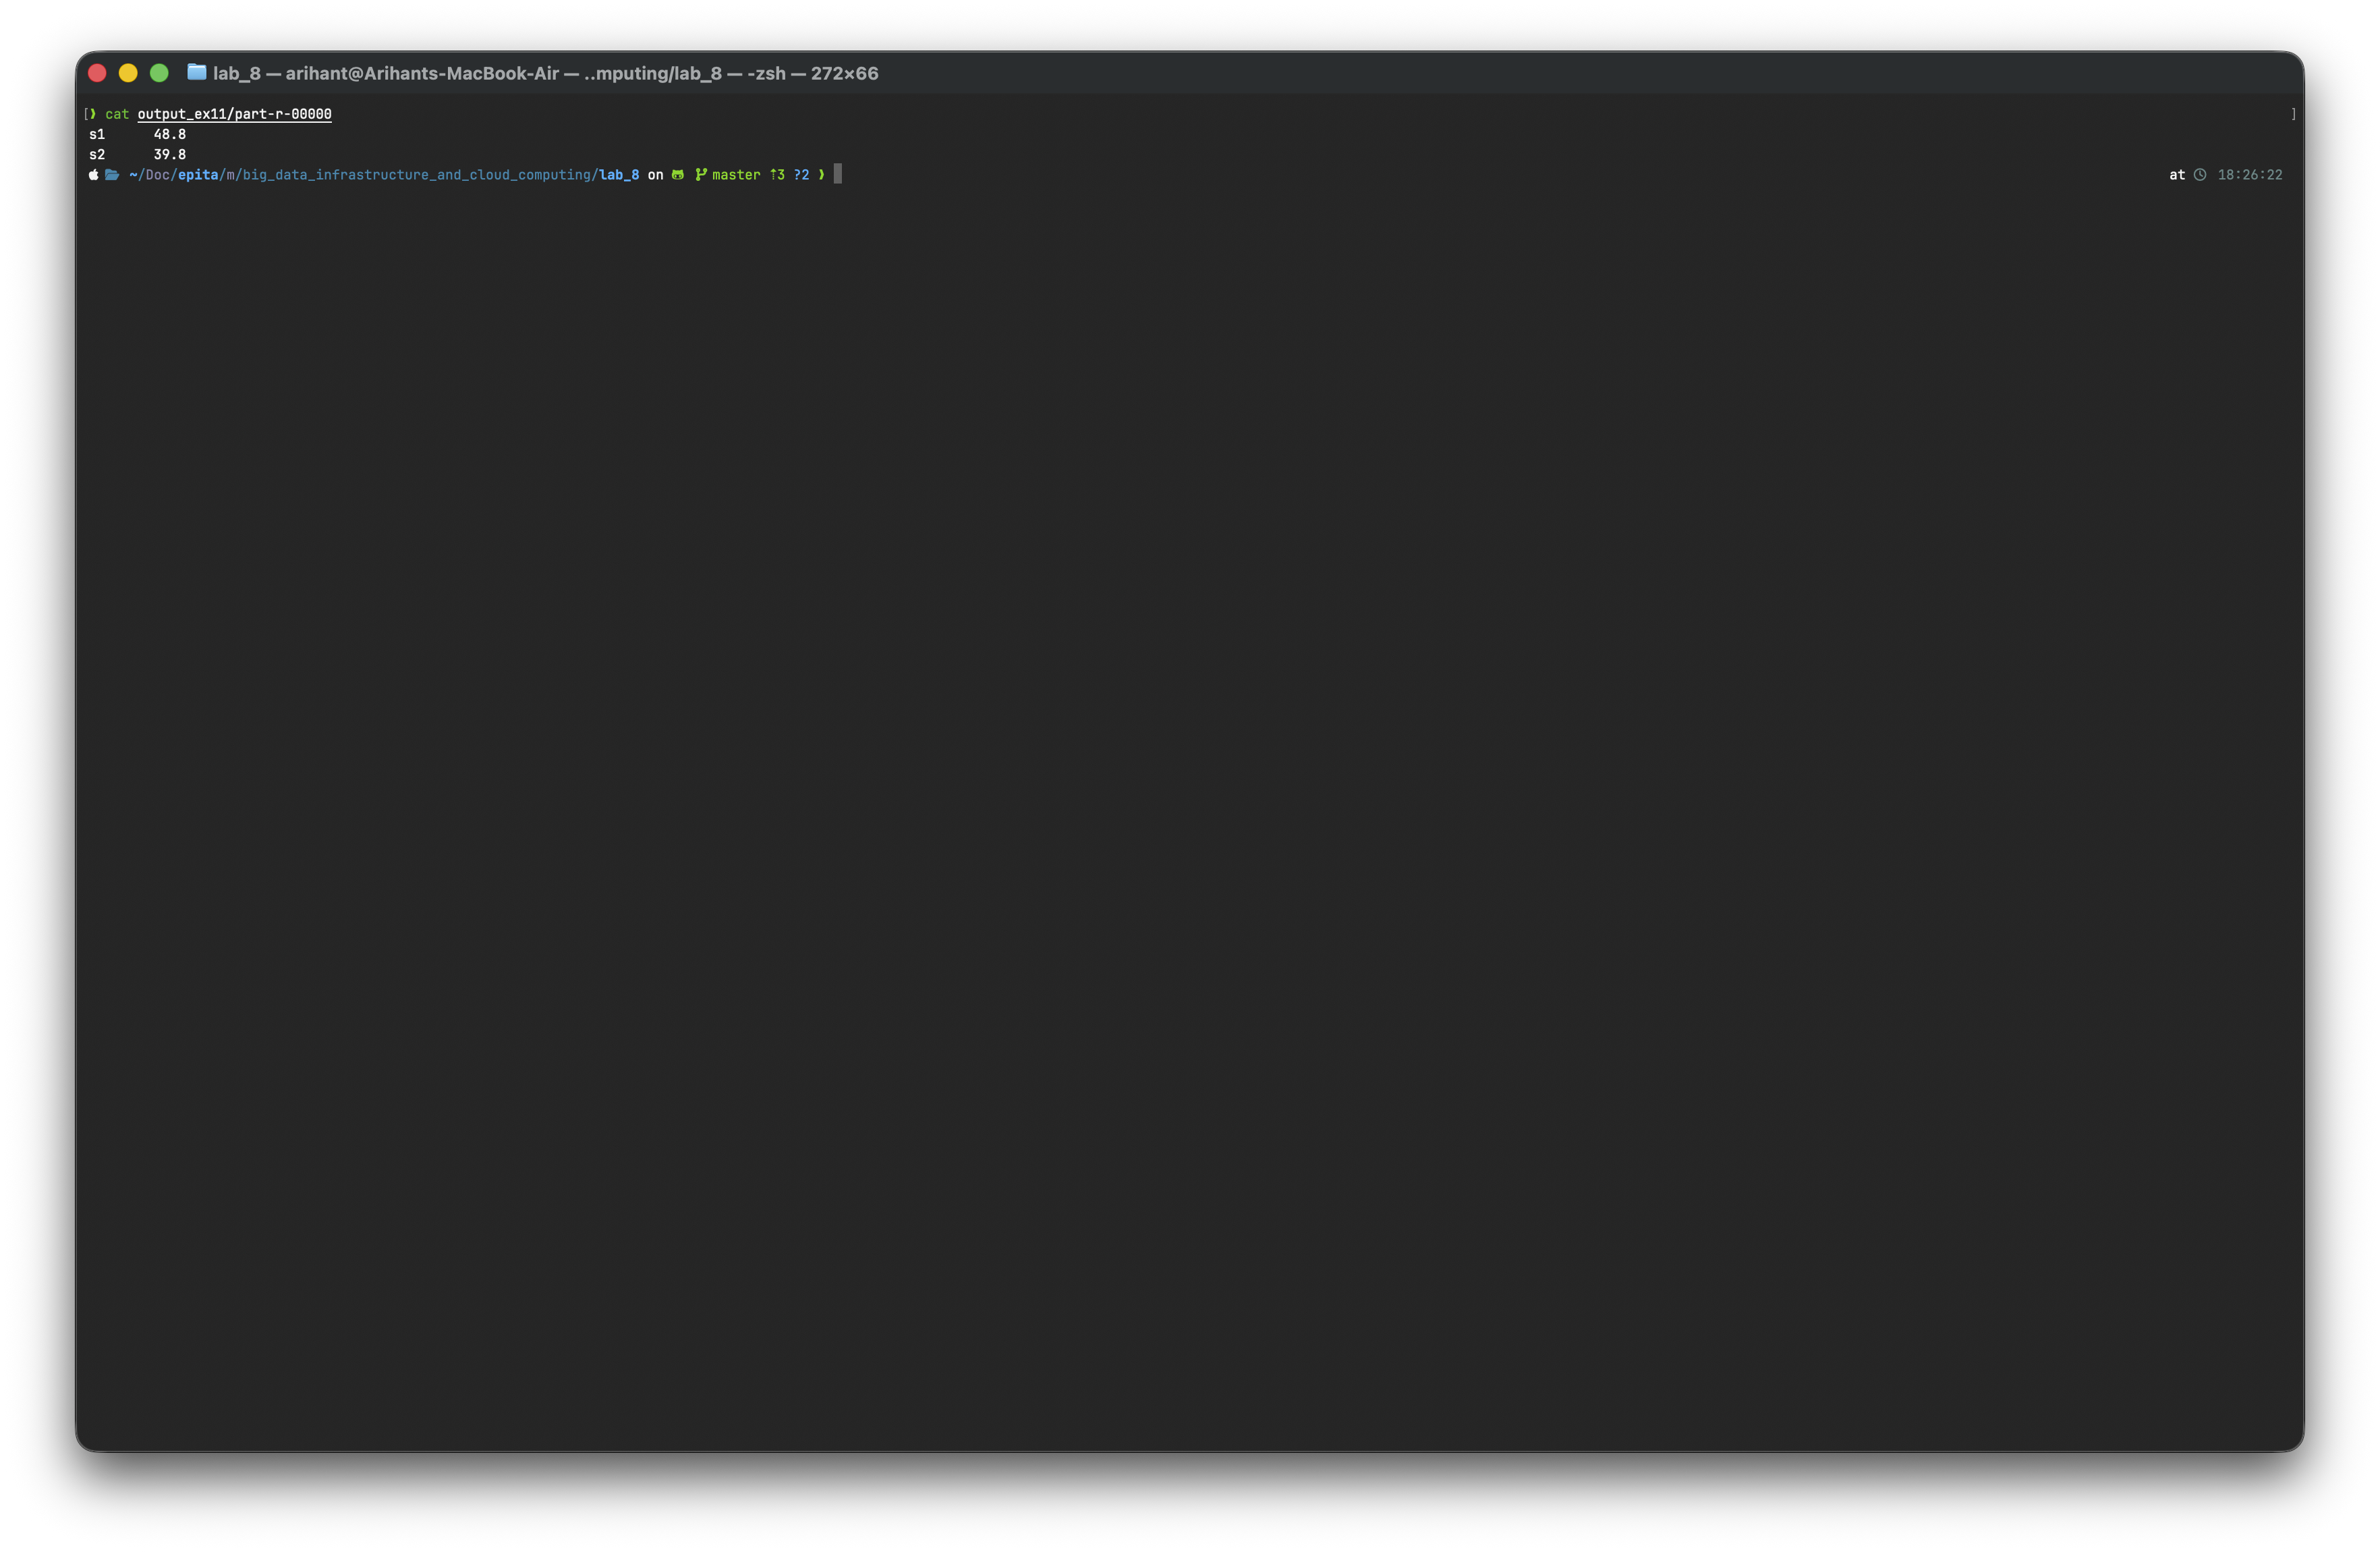
\includegraphics[width=0.75\textwidth]{screenshots/phase3/part-r-0000_ex11.png}
    \caption{Exercise 11 output}
\end{figure}

\section{Top 2 Most Profitable Dates}

\subsection*{Objective}
Find the two dates with the highest total income.

\subsection*{Implementation}
The reducer sums the income for each date and keeps the two largest totals.

\subsection*{Result}
The top two dates in the sample data are \texttt{2024-01-04} and \texttt{2024-01-05}.

\begin{figure}[H]
    \centering
    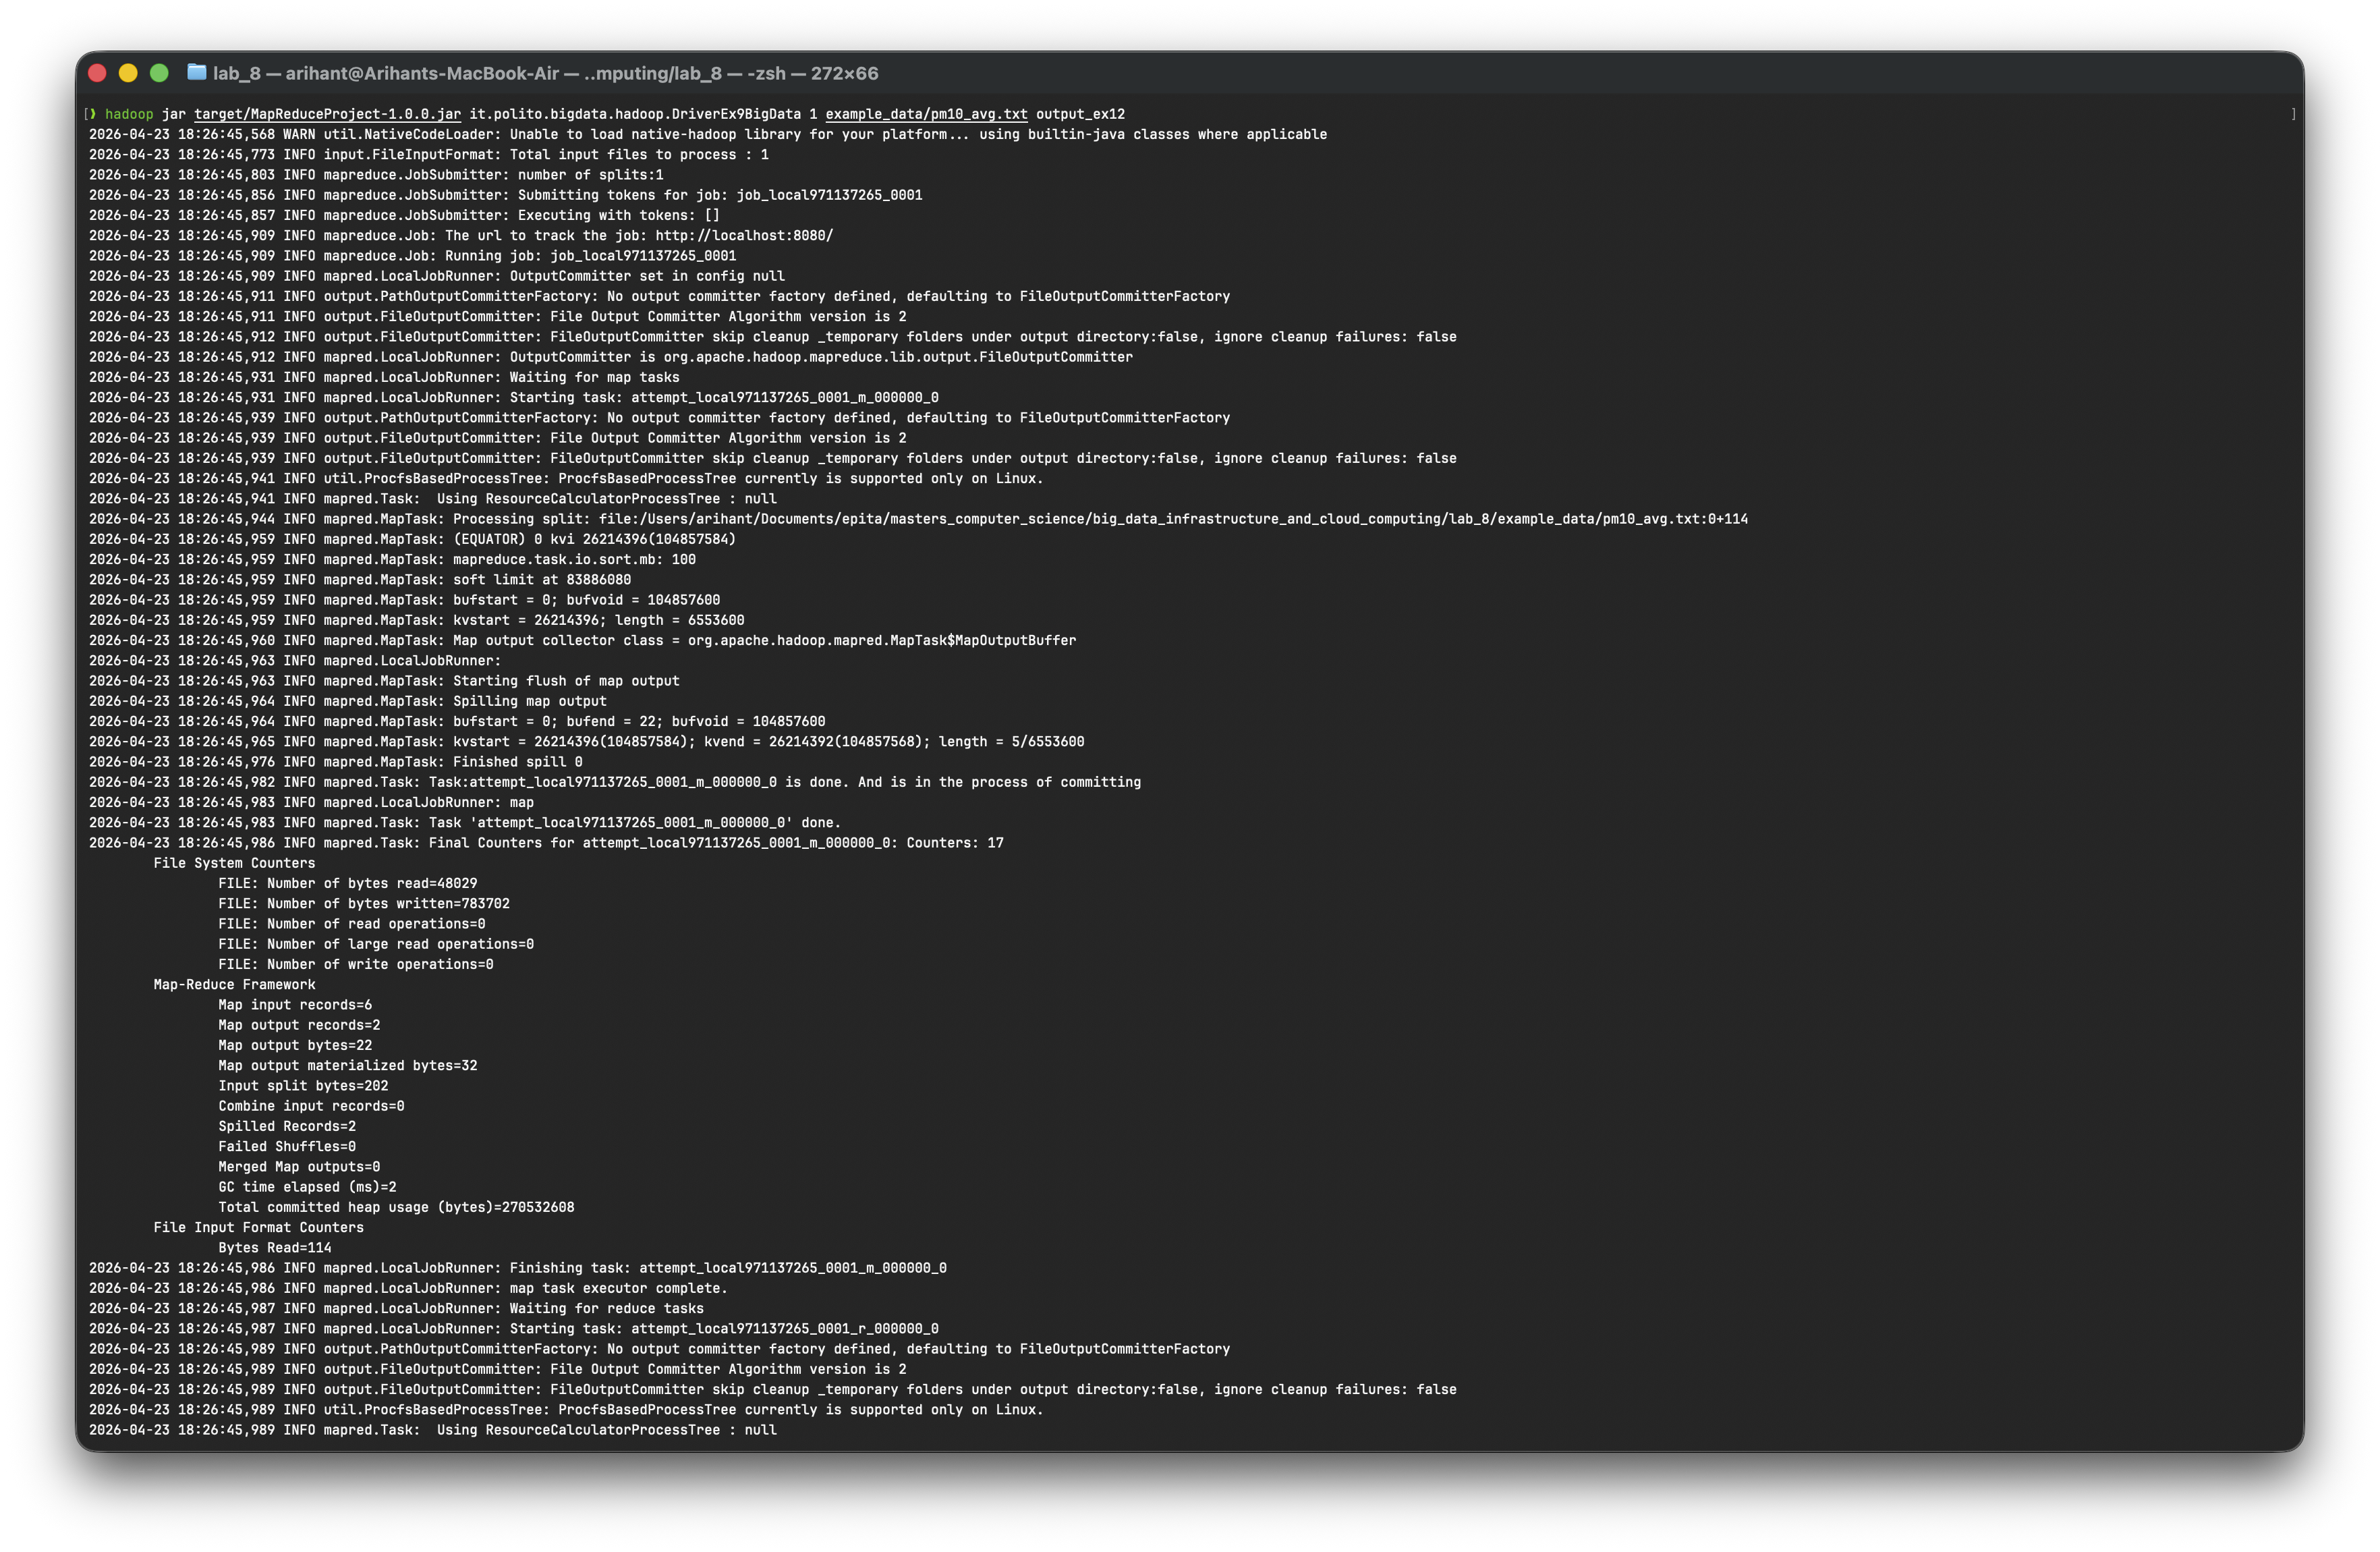
\includegraphics[width=0.75\textwidth]{screenshots/phase3/hadoop_cmd_ex12.png}
    \caption{Exercise 12 command}
\end{figure}

\begin{figure}[H]
    \centering
    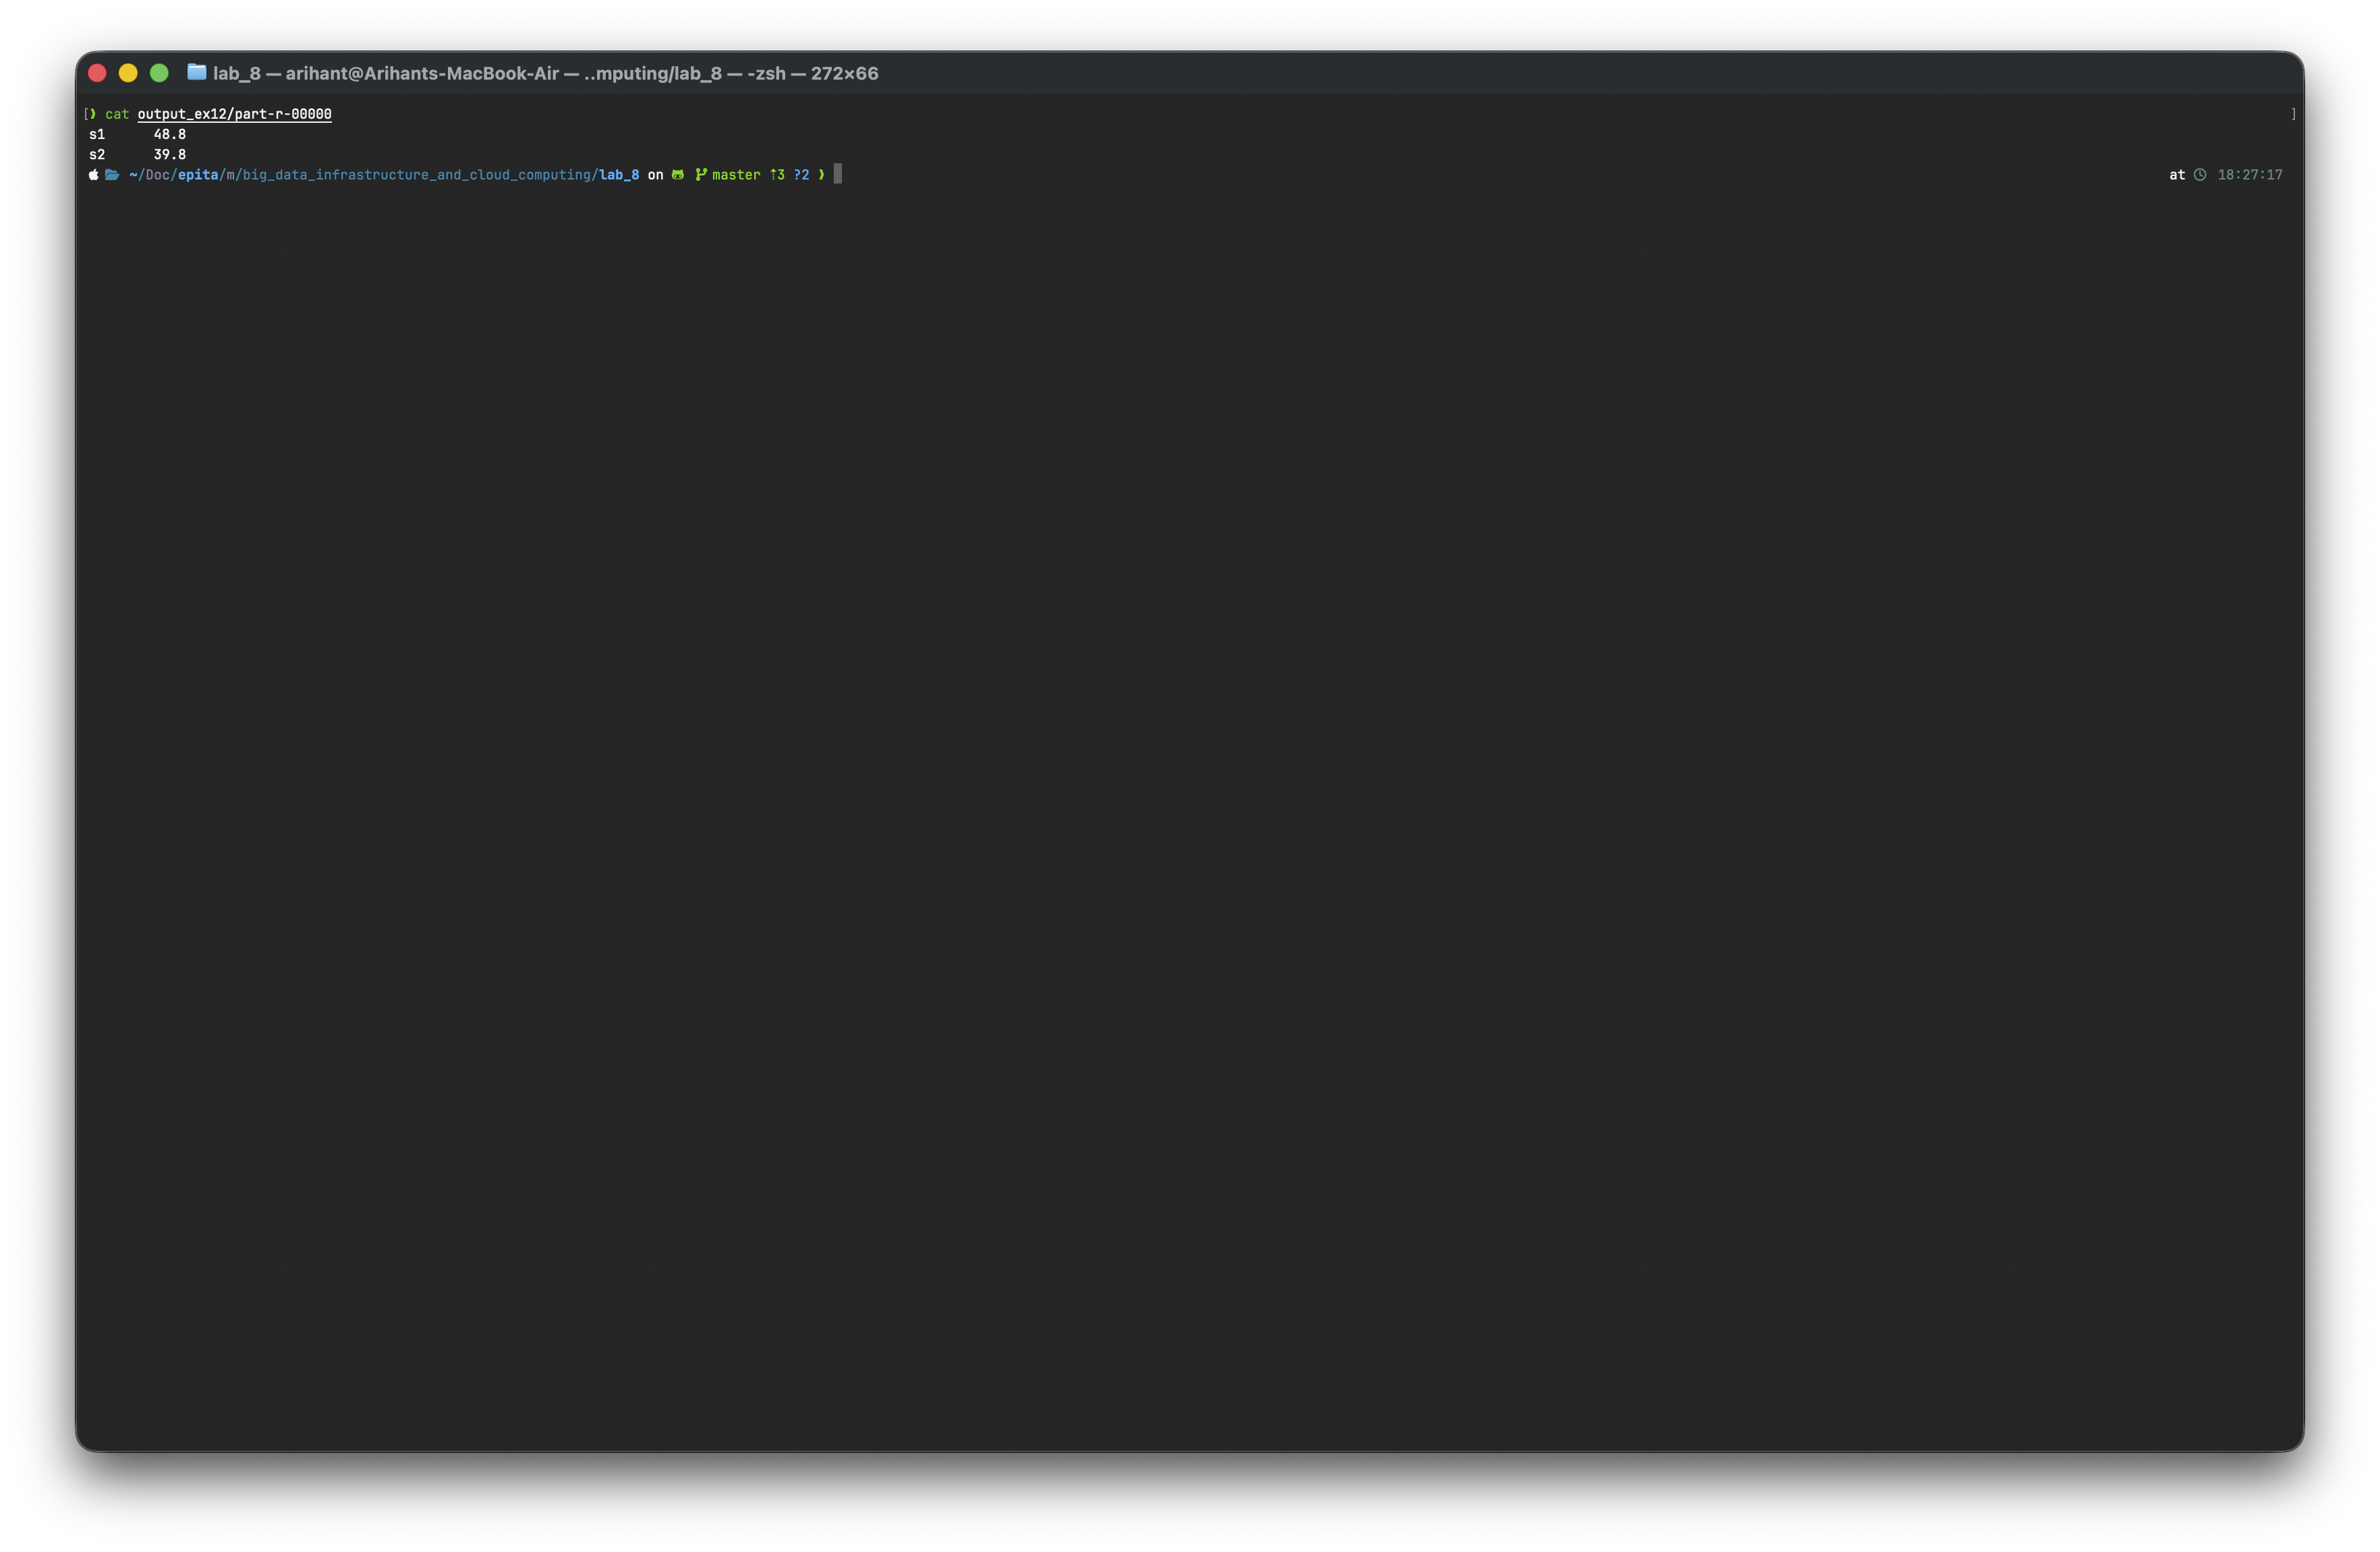
\includegraphics[width=0.75\textwidth]{screenshots/phase3/part-r-0000_ex12.png}
    \caption{Exercise 12 output}
\end{figure}

\section*{Conclusion}
\addcontentsline{toc}{section}{Conclusion}

The first 12 exercises of Lab 8 were implemented with the Hadoop New Style API, built with Maven, and tested on local sample data. The report includes the command and output screenshots saved under the \texttt{report/screenshots} folder.

\end{document}
